%% LyX 1.6.7 created this file.  For more info, see http://www.lyx.org/.
%% Do not edit unless you really know what you are doing.
\documentclass[12pt,a4paper,ngerman,english,intoc,bibtotoc,idxtotoc,BCOR10mm,titlepage,tablecaptionabove,oneside]{scrbook}
\usepackage{lmodern}
\renewcommand{\sfdefault}{lmss}
\renewcommand{\ttdefault}{lmtt}
\usepackage[T1]{fontenc}
\usepackage[latin9]{inputenc}
\usepackage{fancyhdr}
\pagestyle{fancy}
\setcounter{secnumdepth}{3}
\setlength{\parskip}{\medskipamount}
\setlength{\parindent}{0pt}
\usepackage{babel}

\usepackage[authoryear]{natbib}

\def\CC{{C\nolinebreak[4]\hspace{-.05em}\raisebox{.4ex}{\tiny\bf ++}}}

\usepackage{datetime}
\renewcommand{\dateseparator}{.}

\usepackage{trackchanges}
\addeditor{JB}
\addeditor{DD}
\addeditor{SD}
\newcommand{\tnfa}{TNF-$\alpha$ }
\newcommand{\sdfonea}{SDF-1$\alpha$ }

\usepackage{amsmath}
\usepackage{graphicx}
\usepackage{amssymb}
\usepackage{nomencl}
% the following is useful when we have the old nomencl.sty package
\providecommand{\printnomenclature}{\printglossary}
\providecommand{\makenomenclature}{\makeglossary}
\makenomenclature
\usepackage[unicode=true, 
 bookmarks=true,bookmarksnumbered=true,bookmarksopen=true,bookmarksopenlevel=1,
 breaklinks=false,pdfborder={0 0 0},backref=false,colorlinks=true,citecolor=blue,linkcolor=magenta]
 {hyperref}
\hypersetup{pdftitle={Your Title},
 pdfauthor={Jie Bao},
 pdfsubject={Dissertation zur Erlangung des Doktorgrades der Fakult�t f\"ur Biologie der Albert-Ludwigs-Universit�t Freiburg im Breisgau},
 pdfkeywords={Ph.D. thesis},
 pdfpagelayout=OneColumn, pdfnewwindow=true, pdfstartview=XYZ, plainpages=false}

\makeatletter

%%%%%%%%%%%%%%%%%%%%%%%%%%%%%% LyX specific LaTeX commands.
\pdfpageheight\paperheight
\pdfpagewidth\paperwidth

\DeclareRobustCommand*{\lyxarrow}{%
\@ifstar
{\leavevmode\,$\triangleleft$\,\allowbreak}
{\leavevmode\,$\triangleright$\,\allowbreak}}

%%%%%%%%%%%%%%%%%%%%%%%%%%%%%% User specified LaTeX commands.
% print no date
\date{}

% increase link area for cross-references and autoname them
\AtBeginDocument{\renewcommand{\ref}[1]{\mbox{\autoref{#1}}}}
\newlength{\abc}
\settowidth{\abc}{\space}
\addto\extrasenglish{
 \renewcommand{\equationautorefname}{Eq.\hspace{-\abc}}
 \renewcommand{\sectionautorefname}{Sec.\negthinspace}
 \renewcommand{\subsectionautorefname}{Sec.\negthinspace}
 \renewcommand{\subsubsectionautorefname}{Sec.\negthinspace}
 \renewcommand{\figureautorefname}{Fig.\negthinspace}
 \renewcommand{\tableautorefname}{Tab.\negthinspace}
}

% in case somebody want to have the label "equation"
%\renewcommand{\eqref}[1]{equation~(\negthinspace\autoref{#1})}

% that links to image floats jumps to the beginning
% of the float and not to its caption
\usepackage[figure]{hypcap}

% the pages of the TOC is numbered roman
% and a pdf-bookmark for the TOC is added
\let\myTOC\tableofcontents
\renewcommand\tableofcontents{%
  \frontmatter
  \pdfbookmark[1]{\contentsname}{}
  \myTOC
  \mainmatter }

% make caption labels bold
\setkomafont{captionlabel}{\bfseries}
\setcapindent{1em}

% enable calculations
\usepackage{calc}

% fancy page header/footer settings
\renewcommand{\chaptermark}[1]{\markboth{#1}{#1}}
\renewcommand{\sectionmark}[1]{\markright{\thesection\ #1}}
%\lhead[\fancyplain{}{}]{\fancyplain{}{\rightmark}}
\rhead[\fancyplain{}{\leftmark}]{\fancyplain{}{}}
\lfoot[\thepage]{}
\rfoot[]{\thepage}
\cfoot{}

% increase the bottom float placement fraction
\renewcommand{\bottomfraction}{0.5}

% avoid that floats are placed above its sections
\let\mySection\section\renewcommand{\section}{\suppressfloats[t]\mySection}

% widen the space for the nomenclature entry labels
\renewcommand{\nomlabelwidth}{2.5cm}

\makeatother

\begin{document}
\selectlanguage{ngerman}%

\subject{Dissertation zur Erlangung des Doktorgrades der 
Fakult�t f\"ur Biologie
der Albert-Ludwigs-Universit�t Freiburg im Breisgau}

\selectlanguage{english}%

\title{A Network View of the Dynamic Transcriptome Response}


\author{Jie Bao}


\date{}

\selectlanguage{ngerman}%

\publishers{
\includegraphics[width=0.4\columnwidth]{fig/Uni_Logo-Grundversion_E1_A4_CMYK}\vspace{\baselineskip}\\
Albert-Ludwigs-Universit�t Freiburg im Breisgau\\
Fakult�t f\"ur Biologie\\
%Institut f�r zzz\vspace{-3cm}
}


\lowertitleback{\textbf{Dekan}\smallskip{}
\\
Prof. Dr. Ad Aertsen\bigskip{}
\\
\textbf{Promotionsvorsitzender}\smallskip{}
\\
Prof. Dr. Samuel Rossel\bigskip{}
\\
\textbf{Betreuer der Arbeit}\smallskip{}
\\
Dr. Hauke Busch\bigskip{}
\\
\textbf{Datum der Promotion (only necessary for final publication)}\smallskip{}
\\
xx.yy.zzzz}

\selectlanguage{english}%

\maketitle

\thispagestyle{empty}
\setcounter{page}{0}
\vspace*{\fill}
\begin{quote}
The whole is more than the sum of its parts. 
\begin{flushright}
--- Aristotle\\
\end{flushright}
\end{quote}
\vskip 1in
\begin{quote}
Theorie ohne Praxis ist 
wirkungslos, Praxis ohne Theorie ist blind.
\begin{flushright}
--- Immanuel Kant\\
\end{flushright}
\end{quote}
\vfill
\noindent

\cleardoublepage{}

\lhead[\fancyplain{}{}]{\fancyplain{}{\rightmark}}

\tableofcontents{}
\listoffigures

\cleardoublepage{}

\pagestyle{plain}

\begin{itemize}
  \item introduction
  \begin{itemize}
    \item signal flow: protein interaction network $\rightarrow$ transcriptome
    \item failure of biomarker
    \item complexity can only be understood within the
      network context~\citep{Barabasi2012}, Understanding a complex network's 
      structure is beneficial to understanding its function
  \end{itemize}
  \item network dynamics and topology
  \begin{itemize}
    \item fireworks: sequence of events, dynamics
    \item elephant in the room: what we can and cannot see from
    the transcriptome data
    \item gene expression heavy-tailed distributed, discuss 
    bimodal distribution 
    \item normalization assumption: most genes do not change
    expressions
    \item few genes respond: sparsity assumption in reverse-%
    engineering
    \item Network inference in the yeast is already hard because absence of correlation
    between TF expression and activity~\cite{Marbach2012}
    \item CRNT: structure of the reaction network determines the number and type of
    steady states
  \end{itemize}
  \item signal flow
  \begin{itemize}
    \item TF important in disease, but not detectable: many of the TFs that regulate physiological
    targets are constitutively present, and their activity is determined
    by posttranslational modifications such as phosphorylation%
    ~\cite{Messina2004}
  \end{itemize}
  \item conclusions
\end{itemize}

%\include{Summary}
%
%\include{Zusammenfassung}
%
%\cleardoublepage{}
%
%\pagestyle{fancy}\lhead[\fancyplain{}{\chaptername\;\thechapter}]{\fancyplain{}{\rightmark}}
%
%\include{chapter-1}

% $Id: network.tex 2 2012-09-13 23:13:00Z jbao $
\chapter{Network dynamics and topology}

Cells initiate and control decisions like migration, proliferation or differentiation through the intricate, yet
coordinated, regulation of large gene interaction networks. 
As a consequence, there is  well orchestrated time-sequential regulation of protein pathways, resulting in and regulated by a  global change in gene expression.
Gaining insight into the necessary and suffient regulators controlling cellular decisions  is therefore difficult. 
The central questions are, how to bridge the large data set to regulator or key players, how does the cell come to unique and well defined decisions despite the underlying complexity?

Systems theory points to ways how complex systems are regulated and obey common rules with respect to their organisation and dynamic responses~\citep{Kauffman1993}. 
In order to tackle the complexity of such systems, 
one usually works with
an abstract
representation or a graph consisting of different molecules as nodes and the 
interactions among them as edges. In order to understand the
behavior of complex systems, one has to understand both
the topological and dynamical properties of networks. In this chapter, we first
introduce some graph theoretical concepts, we then investigate the dynamics and
topology in \emph{in silico} networks, finally we present a biological application.

\section{Complex networks in biology and beyond}
Biological phenomena are described in the context of a network
at all spatial and temporal scales, from food web~\citep{Williams2000}, 
neuronal network~\citep{White1986}, gene regulatory networks~%
\citep{Kauffman1969,Gama-Castro2008,Abdulrehman2011},
protein-protein interaction networks~\citep{Jeong2001,Stelzl2005}
to metabolic network~\citep{Herrgaard2008}.

The study of networks dates back to the K\"onigsberg
problem from Leonhard Euler in the 18th century. The initial
problem deals with seven bridges across the river in the city
of K\"onigsberg, and the aim is to find a walk through the 
city that would cross each bridge once and only once, to which
Euler proved that there is no solution. For a long time,
graph theory remains a specialized and abstract mathematical 
discipline. Not until the publication of the first 
small-world network model~\citep{Watts1998} did people
realize that there is a class of networks, which is neither
purely random nor purely regular and can represent most of
the real-world structures, ranging from Internet, power grid
to collaboration graph of film actors, and also biological
networks.

Study of biological networks has been largely inspired by the theoretical 
analyses of other types of networks~\citep{Barabasi2004}. In recent years, 
there is also increasing interest in the comparison between biological and
other networks. For instance, the transcriptional regulatory network of 
\emph{E. coli} is found to have a triangle-like hierarchical 
structure, whereas the Linux kernel displays rather an inverse-triangle
hierarchy, which again is due to different design principles of the two 
systems: robustness for biological systems and cost effectiveness for 
software systems~\citep{Yan2010}.
Such findings highlight the hypothesis of \emph{form follows function}, or 
the function of complex networks can be attributed to their distinct structural 
properties.

\section{Network topology}
There are a variety of measures that characterize the topology of networks,
some capture local network topology, yet others are global topology measures.

\subsection{Topological measures}

\subsubsection{Degree and degree distribution}
The \emph{degree} (or connectivity) $k_i$ of a node $i$ is the number of edges 
connecting the node, in case of directed networks, one further distinguishes
between incoming ($k_i^{in}$) and outgoing degree ($k_i^{out}$). Then the total 
degree is defined as $k_i = k_i^{out} + k_i^{in}$. A list of the node degrees 
of a network is called the \emph{degree sequence}.

The \emph{degree distribution} $P(k)$, or the fraction of nodes in the graph 
$G$ having degree $k$, is probably the most basic topological 
characterization of a graph. It has been shown that the degree distribution of
a neuronal network determines its global oscillatory state~\citep{Roxin2011}, 
and the number of driver nodes in a network is determined mainly by the 
network's degree distribution, assuming linear dynamics at
individual nodes~\citep{Liu2011}.

\subsubsection{Shortest path and betweenness}
\emph{Shortest paths} $d_{ij}$ from node $i$ to node $j$ play an important 
role in the transport and communication 
within a network. Although highly efficient algorithm exists to perform
route planning such as in Google Maps~\citep{Sanders2005}, common algorithms
for calculating shortest paths are Dijkstra's algorithm for weighted networks
and the breadth-first search for unweighted networks.

An extension of the shortest path is a measure of the importance of a given 
node defined by the sum of the fraction of all-pairs shortest paths that pass 
through it, or the 
\emph{betweenness} $b_i$ of a node $i$ is given by
\begin{equation}
b_i = \sum_{s,t \in N} \frac{\sigma(s,t|i)}{\sigma(s,t)},
\end{equation}
where $N$ is the set of nodes, $\sigma(s,t)$ is the number of shortest paths 
between node $s$ and $t$, and $\sigma(s,t|i)$ is the number of those paths 
passing through the node $i$ other than $s$ and $t$.

\subsubsection{Motif}
A \emph{network motif} $M$ is a pattern of interconnections occurring in complex 
networks at a number that is significantly higher than those in randomized 
networks~\citep{Milo2002,Shen-Orr2002}. The statistical significance of M is 
then described by the $Z$-score, defined as
\begin{equation}
Z_M = \frac{n_M - \langle n_M^{rand} \rangle}{\sigma_{n_M^{rand}}},
\end{equation}
where $n_M$ is the number of times the subgraph $M$ appears in $G$, and 
$\langle n_M^{rand} \rangle$ and $\sigma_{n_M^{rand}}$ are, respectively, 
the mean and 
standard deviation of the number of appearances in the randomized network ensemble.
Motifs have been strongly linked to the information processing in networks, 
for example, the incoherent feedforward loop was shown to be able to detect
fold change in the input signal~\citep{Goentoro2009}.

\subsubsection{Community}
A \emph{network community} or module is a subnetwork with many edges joining
nodes of the same cluster and comparatively few edges joining nodes of 
different clusters. Since such communities can be considered as fairly 
independent compartments of a graph, they are usually also assigned 
a similar function, e. g., individual tissues or organs in the human body,
pathways within the cellular signal transduction network, a group of people
with common interest within the social network~%
\citep{Fortunato2010,Newman2012}.

There are now a zoo of algorithms to detect network communities, probably one
of the most influential methods is the algorithm proposed by \cite{Girvan2002},
which aims at the identification of edges lying between communities and their 
successive removal, a procedure that after some iterations
leads to the isolation of the communities. Most recently, \cite{Ahn2010b} 
suggested that each node in a network can in principle belong to more than 
one functional group, they therefore reinvented the definition of communities 
as groups of links rather than nodes and demonstrated this approach can uncover
natural overlap while revealing hierarchical organization of the network.

\subsection{Scale-free networks}
Together with the small-world network model, the scale-free network model~%
\citep{Barabasi1999} has
also attracted much attention in the research community. The basic idea of 
how a scale-free network and its power-law degree distribution comes into
existence is called preferential attachment. In other words, at each time
step of a growing network, a new node is added to a certain node in the 
network based on the probability that is proportional to the degree of the
given node, i.e. strongly connected nodes will get more and more connections,
popular nodes will be even more attractive. Such a model is able to reproduce
the power-law degree distribution observed in scale-free networks.

However, recent years have seen a critical assessment of the original 
scale-free model. On the one hand, several rigorous statistical analyses~%
\citep{Clauset2009,Khanin2006a} have shown that methods used to fit power-laws, such as 
least-squares, can produce substantially inaccurate estimates of the 
parameters. The authors concluded that in general the cumulative distribution
function is more robust than the probability distribution function against 
fluctuations due to finite sample sizes, especially in the tail of the 
distribution. It is also extremely difficult to distinguish between
the log-normal and power-law distribution. These results cast doubt on the
validity of most empirical characterization of power-law degree distribution
and the significance of classifying scale-free networks according to such
degree distributions.

On the other hand, there is now increasing evidence that mechanisms other than
preferential attachment can also lead to the empirical power-law degree 
distribution~\citep{Caldarelli2002}. For instance, a model of unspecific 
binding between proteins results exactly in a scale-free protein-protein 
interaction network~\citep{Deeds2006}.

\section{Network dynamics}
Here the network dynamics refers specifically to the dynamic response of the 
gene regulatory network. Such data are usually obtained from the microarray
time series. Microarray technology takes advantage of hybridization properties 
of nucleic acids and uses complementary molecules (probes) attached to a solid 
surface 
(chip) to measure the quantity of specific nucleic acid transcripts of 
interest that are present in a sample. A specialized scanner is used to 
measure the amount of hybridized target at each probe, which is reported as an 
intensity~\citep{Gentleman2005}. This intensity value is then interpreted as a
proxy for the level of gene expression. In order to characterize the global 
gene expression given a certain stimulus over time, one can perform the 
hybridization at multiple time points. The ultimate gene expression data are
thus multidimensional time series. Below we provide some of the methods that
can be used to analyse such data.

\subsection{Dimensionality reduction}
Dimensionality reduction is the transformation of high-dimensional data into 
a meaningful representation of reduced dimensionality~\citep{Maaten2009}, 
which is easy to both visualize and interpret. There are a variety of linear
and nonlinear dimensionality reduction algorithms 
(\ref{fig:dimension_reduction}). In this work, we heavily 
focus on the Euclidean distance based multidimensional 
scaling, which is equivalent to principal component analysis%
~\citep{Haerdle2003},
but more intuitive.

\begin{figure}[!ht]
\begin{center}
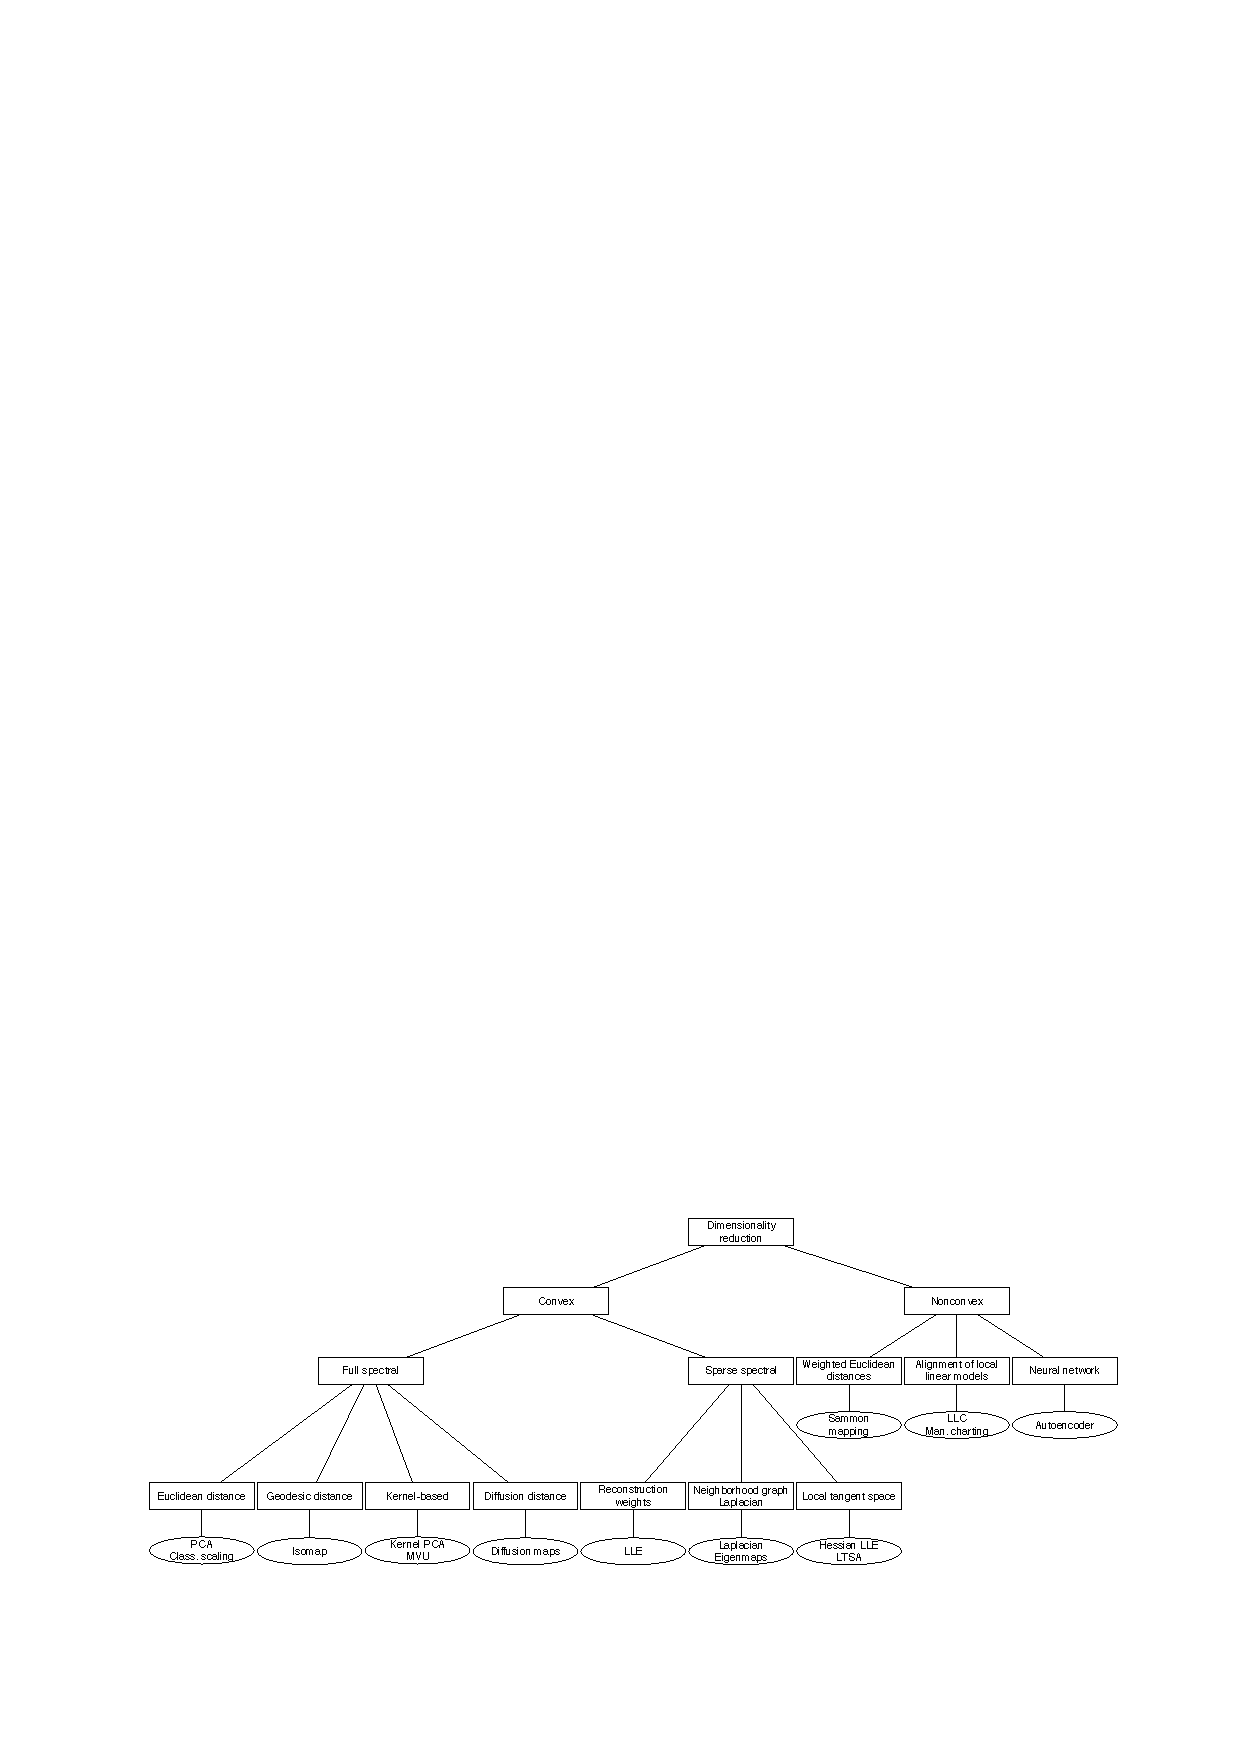
\includegraphics[width=\textwidth]{network/fig/dimension_reduction.pdf}
\end{center}
\caption[Dimensionality reduction algorithms]{
{\bf The taxonomy of dimensionality reduction algorithms.}
A non-exhaustive overview of diverse dimensionality reduction
techniques, taken from \cite{Maaten2009}.
}
\label{fig:dimension_reduction}
\end{figure}

\subsubsection{Multidimensional scaling}
Multidimensional scaling (MDS) is a family of algorithms that produces a spatial
representation of the dissimilarities between a number of entities $x_l^i \in 
\boldsymbol{X}_{n \times q}$ in $q$-dimensional space. In 
principle, MDS takes as input a symmetric $n \times n$ matrix 
\begin{equation}
  \boldsymbol{D} = \sqrt{\sum_{l=1}^q (x_l^i - x_l^j)^2}_{\substack{i \neq j,\\
    i,j=1...n}},
\end{equation}
which
describes the dissimilarities between the high-dimensional
entities. Those entities
are then represented by points in a low-dimensional space $\hat{x}_l^i \in 
\hat{\boldsymbol{X}}_{n \times d}$ ($d$ usually equals $2$ or
$3$ for ease of visualization), which are positioned
such that the pairwise distances between them 
\begin{equation}
  \hat{\boldsymbol{D}} = \sqrt{\sum_{l=1}^d (\hat{x}_l^i - \hat{x}_l^j)^2}_{\substack{
    i \neq j,\\i,j=1...n}}
\end{equation}
reflect as closely as possible  
the original
dissimilarities between the entities. 
The optimization of the spatial configuration is realized by the 
minimization of different stress functions.
We applied
here the HiT-MDS-2 algorithm (\citealp{Strickert2009}), where the
Pearson correlation of the original and the reconstructed distances 

\begin{equation}
  r(\boldsymbol{D}, \hat{\boldsymbol{D}}) = \frac{\sum_{i \neq j}^n (d_{ij} - \mu_{\boldsymbol{D}}
    ) \cdot (\hat{d}_{ij} - 
    \mu_{\hat{\boldsymbol{D}}})}{\sqrt{\sum_{i \neq j}^n (d_{ij} - \mu_{\boldsymbol{D}})^2} 
    \cdot \sqrt{
    \sum_{i \neq j}^n (\hat{d}_{ij} - \mu_{\hat{\boldsymbol{D}}})^2}}
\end{equation}
is maximized using a gradient descent approach.
Perticularly, $\boldsymbol{D} = (d_{ij})_{i,j=1...n}$ is Euclidean distance matrix of the
gene expression time series, and $\hat{\boldsymbol{D}} = (\hat{d}_{ij})_{i,j=1...n}$ 
is the 
Euclidean distance matrix of the reconstructed low-dimensional points. 
$\mu_{\boldsymbol{D}}$ and $\mu_{\hat{\boldsymbol{D}}}$ are the mean of matrix $\boldsymbol{D}$
and $\hat{\boldsymbol{D}}$ respectively.
\begin{eqnarray}
  \mu_{\boldsymbol{D}} = \frac{2}{n (n-1)} \sum_{i<j}^N d_{ij},\\
  \mu_{\hat{\boldsymbol{D}}} = \frac{2}{n (n-1)} \sum_{i<j}^N \hat{d}_{ij}.
\end{eqnarray}
%A stress function 
%\begin{equation}
%  s = -r(\boldsymbol{D}, \hat{\boldsymbol{D}})
%\end{equation}
%is minimized by gradient descent.
Throughout this work, the number of optimization cycles is fixed to be $100$.
The final configuration is centered, normalized by the largest dimension variance,
and rotated by Principal Component Analysis.

\subsubsection{Response strength metric}
\label{sec:response_strength}
In order to quantify the response strength of a single gene, we make use of 
MDS, namely by fitting a skewed Gaussian distribution (\citealp{Azzalini2003}) 
to the 2-D projection
of gene expression time series and assigning a $p$-value to each
gene according to its probability of being drawn from the fitted distribution.
We further take the negative logarithmic of the $p$-values as the response
strength metric. In so doing, a gene located at the periphery of the MDS
projection has a small $p$-value and thus a large response strength, whereas
central genes have small response strengths.

A multivariate skewed Gaussian distribution is defined as follows, suppose
$X$ is a $d$-dimensional random variable with a probability density function
\begin{equation}
f(X) = 2 \phi_d (X;\Omega) \ \Phi(\alpha^{\mathrm{T}} X), \quad X \in \mathbb{R}^d,
\label{eq:sn}
\end{equation}
where $\phi_d(X;\Omega)$ is the $N_d(0,\Omega)$ normal density function at $X$
with the correlation matrix $\Omega$, $\Phi(\alpha^{\mathrm{T}} X)$ is the 
cumulative distribution function of $N(0,1)$ evaluated at $\alpha^{\mathrm{T}} X$.
$\alpha$ is the shape parameter since when $\alpha=0$, Eq.~\ref{eq:sn} becomes
the regular normal probability density function again. $X$ can be further
linear transformed to
\[
Y = \xi + \omega X
\]
to include the location and scale parameter, $\xi$ and $\omega$ respectively.

Fitting of the skewed Gaussian distribution is performed with
the maximum likelihood method as implemented in the 
\texttt{R}
library \texttt{sn}, version 0.4-16.

\subsection{Modelling time series}
Another method to determine the dynamic response of a certain
gene is based on the work of \cite{Mar2009}. The difficulty 
in analyzing microarray time series data comes from the lack
of replicates in general at each time point. In order to 
circumvent this problem and increase the statistical power,
we take into account all data points in a time series at the
same time.

More specifically, we fitted cubic regression models to each 
individual gene expression profile. A cubic model was chosen 
because of the moderately large number of time points 
available to fit a model with four to eight parameters. 
For a single gene, both a full model and a reduced model are 
fitted to its time-course expression profiles under the 
stimulation and control condition. The full model specifies 
a set of parameters that capture the time-dependent curvature
of a gene's expression profile for each separate condition. 
In this way, the full model assumes that the expression 
profile is different across the two conditions, or

\subsection{Heave-tail response distribution}
Based on both the multidimensional scaling and full/reduced
model approach, we observe an invariant response pattern that only few genes are strongly induced upon stimulation, while the majority reacts
moderately (\ref{fig:response_strength}). 

\begin{figure}[!ht]
\begin{center}
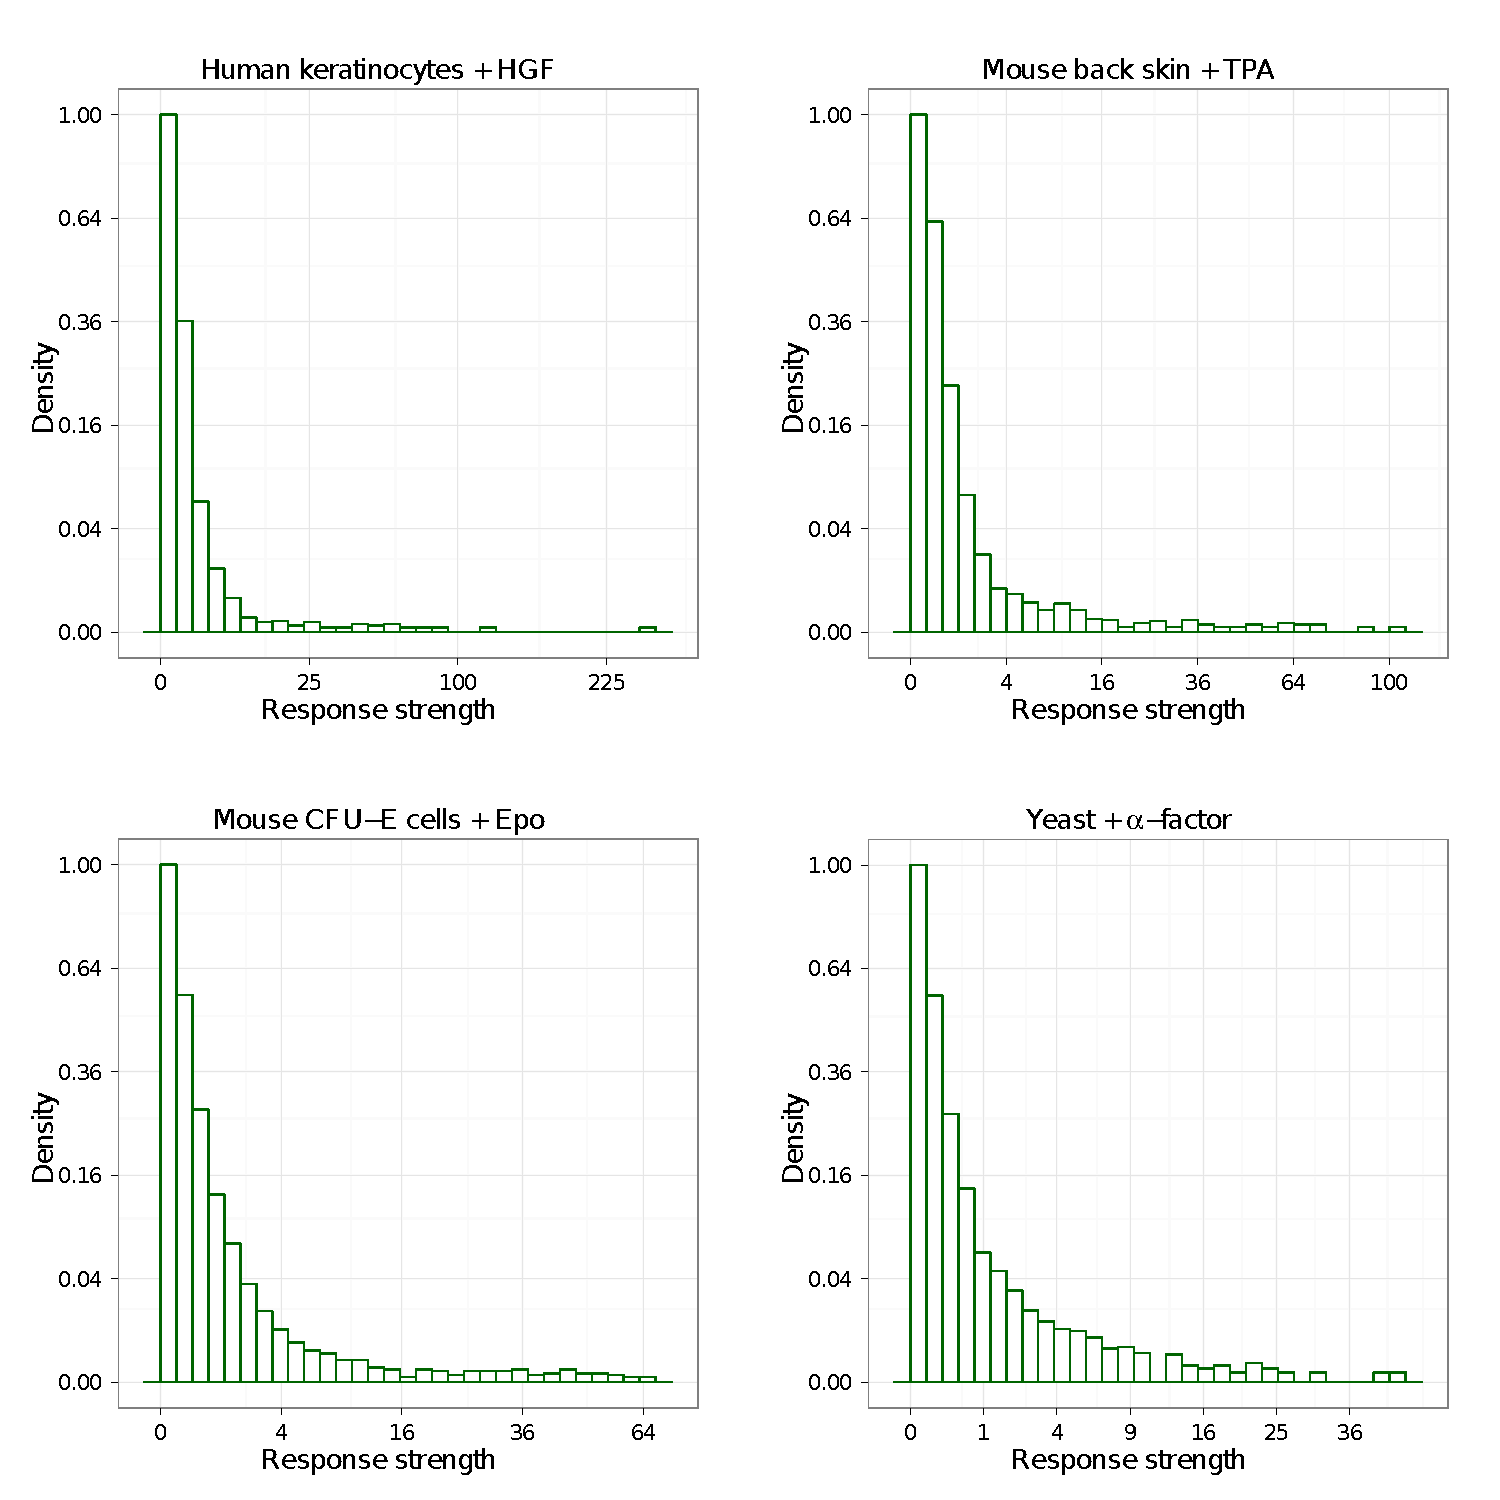
\includegraphics[width=\textwidth]{network/fig/response_all.pdf}
\end{center}
\caption[Heavy-tail distribution of gene response strength]{
{\bf Distribution of gene response strength in different
cell types under different stimulation.}
Gene response strengths are calculated as described in 
\ref{sec:response_strength}, the maximum of each distribution
is normalized to 1. Datasets used in this plot include 
primary human keratinocytes 
stimulated with hepatocyte growth factor (ArrayExpress database 
\texttt{http://www.ebi.ac.uk/arrayexpress/},
accession number E-TABM-440); CFU-E cells from mouse fetal livers stimulated
with Epo (GEO database \texttt{http://www.ncbi.nlm.nih.gov/geo/}, accession
number GSE26151); yeast cells synchronized with 
$\alpha$-factor to study the cell cycle
\\(\texttt{http://genome-www.stanford.edu/cellcycle/data/rawdata/combined.txt}).
}
\label{fig:response_strength}
\end{figure}

The response distributions do not fit well with any of the 
Gaussian, power-law, exponential, log-normal or Weibull distribution, with the closet one being power-law or log-normal
distribution up to a certain range (\ref{fig:response_fit}). 
Nevertheless, the response distributions from various 
biological systems do share the same shape between each 
other (\ref{fig:response_qqplot}). Taken together, gene
responses are indeed heavy-tail distributed, with few
genes strongly regulated and the majority only moderately
regulated, but they do not follow the power-law distribution,
which underlines again the necessity of assessing power-law
distribution on empirical data within a rigorous statistical
framework~\citep{Clauset2009}.

\begin{figure}[!ht]
\begin{center}
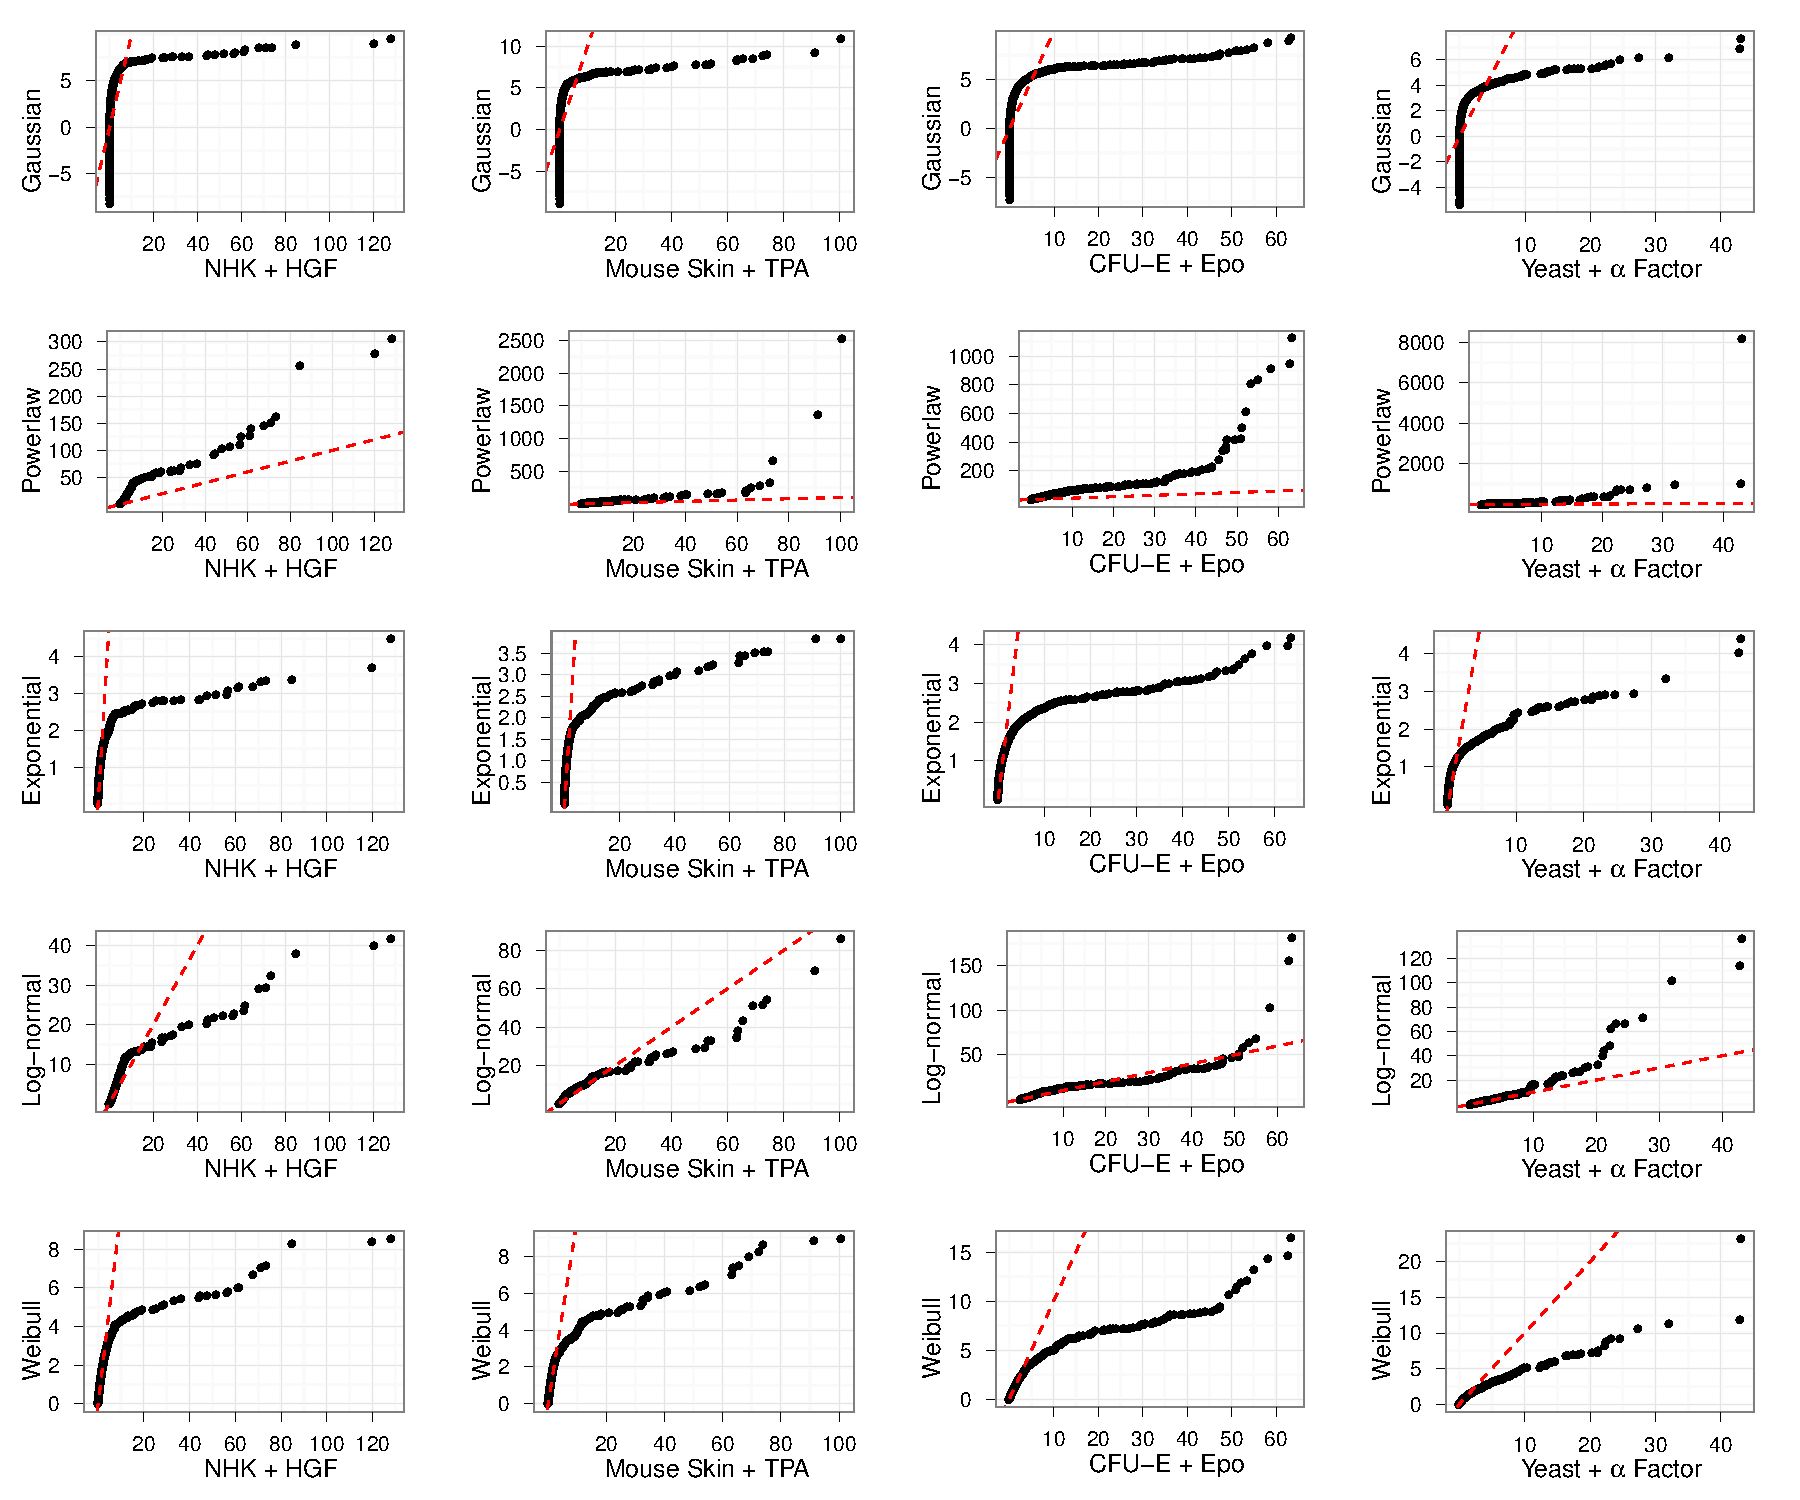
\includegraphics[width=\textwidth]{network/fig/response_fit.pdf}
\end{center}
\caption[Comparison of gene response distributions with
theoretical distributions]{
{\bf Comparison of gene response distributions with 
different theoretical distributions using the quantile-%
quantile plot.}
Biological datasets are the same as in 
\ref{fig:response_strength}, red dashed lines have a slope
of 1 and indicate identity, theoretical distributions 
include Gaussian, power-law, exponential, log-normal and
Weibull distribution~\citep{Clauset2009}.
}
\label{fig:response_fit}
\end{figure}

\begin{figure}[!ht]
\begin{center}
\includegraphics[width=\textwidth]{network/fig/response_qqplot.pdf}
\end{center}
\caption[Comparison of gene response distributions]{
{\bf Pairwise comparison of gene response distributions with 
each other using the quantile-%
quantile plot.} 
Biological datasets are the same as in 
\ref{fig:response_strength}, red dashed lines have a slope
of 1 and indicate identity, the maximal response strength
in each dataset is normalized to 1.
}
\label{fig:response_qqplot}
\end{figure}

One possible cause of the similar be behavior has been the similarity in underlying topology of the gene and protein regulatory network. 

\section{Gene response and connectivity}
Through the simulation of a thermodynamical gene network model, we observed that the response strength of a certain gene negatively correlates with its degree, which is also 
confirmed in various biological data.

\subsection{Synthetic \emph{in silico} networks}
We first describe the construction of \emph{in silico}
network models, both in terms of topology and dynamics.

\subsubsection{Topology}
\begin{itemize}
\item Random: an Erd\H{o}s-R\'enyi graph (\citealp{Erdos1959}) is generated with a probability
  $0.003$ to choose each of the possible edges.
\item Uniform: network with uniform in- and out-degree distributions $k_{in,out} \in 
  \{0,1,...,11\}$ is constructed 
  with the configuration model (\citealp{Newman2001}). 
  In short, a configuration network 
  is constructed in the following manner. Each node $i$ has a desired degree $k_i$, 
  so we imagine that each node has $k_i$ edge ``stubs'' attached to it. Edges are 
  then assigned by randomly choosing two stubs and drawing an edge between them.
\item Small-world: a small-world graph with 1000 nodes 
according to the 
Watts-Strogatz model~\citep{Watts1998} is generated, 
each node is connected
to 5 nearest neighbors in the ring topology and each edge
has a rewiring probability of 0.1. In the end, the 
undirected small-world graph is converted to a directed
graph by randomly assigning edge directions.
\item Scale-free: similar to the case of uniform networks,
except that Poisson in-degree (with $\lambda = 3$) and power-law 
  out-degree distributions ($P(k) = k^{-2.5}$) are assumed as the input
  to the configuration model.
\item Bow-tie: two growing network (GN) graphs 
  (\citealp{Krapivsky2001}) of equal size are first 
  constructed by adding nodes one at a time with an edge to one existing node, 
  which results in two directed trees. With redirection probability $0.1$ the edge
  connects the additional node with the successor node of the random selected target
  node instead of the target node itself. One of the trees is then reversed and 
  concatenated to the other one through the root nodes, such that the resulting
  graph is of the multiple-input multiple-output type.
\end{itemize}
All networks have 1000 nodes and are generated with the Python package NetworkX (\citealp{Hagberg2008}) 
version 1.4, they are further made sure to be connected.

\subsubsection{Dynamics}
We adapted a thermodynamical gene network model 
(\citealp{Marbach2010,Schilstra2002}),
which takes into account the combinatorial control of transcription factors. 
Precisely, the 
gene expression dynamics is defined by 
\begin{equation}
  \dot{x_i}(t) = m_i \cdot f_i(x_j(t)) - d_i \cdot x_i(t), 
\end{equation}
where $x_i(t)$ denotes the expression level of gene $i$ at time $t$, 
$m_i$ is the 
maximum transcription rate, $d_i$ the mRNA degradation rate. $f_i(\cdot)$
is the activation function of gene $i$, it depends on the expression level of 
all the input onto gene $i$ at time $t$, $x_j(t)$ and is the sum of relative 
activations for
different binding states. In general, for $N$ input genes, there are altogether
$2^N$ possible binding states and
\begin{equation}
  \displaystyle f_i(x_j) = \sum_{m=0}^{2^N-1} \alpha_m \theta_m,
\end{equation}
$m$ can be interpreted as an $N$-digit binary number (with padding $0$s) 
and represents one perticular binding state, with the $i$-th
digit indicating the binding state of the $i$-th input gene, namely $0$ for unbound
and $1$ for bound. $\alpha_m$ is the relative activation of state $m$,
$\theta_m$ is the joint probability of state $m$: 
\begin{equation}
  \theta_{m} = \prod_j \frac{x_j^{n_{ij}}}{k_{ij}^{n_{ij}}+x_j^{n_{ij}}}
    \cdot \prod_k \frac{k_k^{n_{ik}}}{k_{ik}^{n_{ik}}+x_k^{n_{ik}}}
\end{equation}
where the probability of a single transcription factor bound to the gene is 
modelled by a Hill function,
$n$ is the Hill coefficient and $k$ is the dissociation constant, at which the
saturation is half-maximal or the transcription factor is bound $50\%$ of the time.
$x_j$ are the bound transcription factors of $x_i$ and $x_k$ the unbound ones.

Time series are simulated by first finding the steady state, where the absolute
concentration change is smaller than $10^{-5} + 10^{-3} \cdot x_i$ for each gene
or the maximal time of $500$ is exceeded. Afterwards, the basal activation $\alpha_0$
is randomly perturbed and the gene expression dynamics is simulated for a total
time of $200$ with $10$ as the time interval and the
steady state as the initial condition.

\CC{} code of the model adapted from GeneNetWeaver (\citealp{Schaffter2011})
is available upon request.

\subsubsection{Rewiring}

\subsection{Topology determines dynamics}
We investigate the influence of network topology on the immediate, dynamic gene response in networks. 
Using biologically meaningful networks of \emph{E. Coli} and 
the budding yeast \emph{S. cerevisiae} generated 
\emph{in silico}, we show that topology has a significant influence on the dynamics, scaling with size. Hub genes are not responding, while weakly connected genes are 

Our results demonstrated that genes with a high level of change in expression are more likely to be peripheral nodes (low connectivity) in the network, whereas hubs (nodes with higher connectivity) and superhubs (nodes that link hubs) tend to have a lower level of change in expression. 
To analyze the biological roles of the modulated genes, we assessed the Gene Ontology (GO) of nodes and hubs. Our analysis identified different annotations of mole- cular functions based on the topological classifications.

\begin{figure}[!ht]
\begin{center}
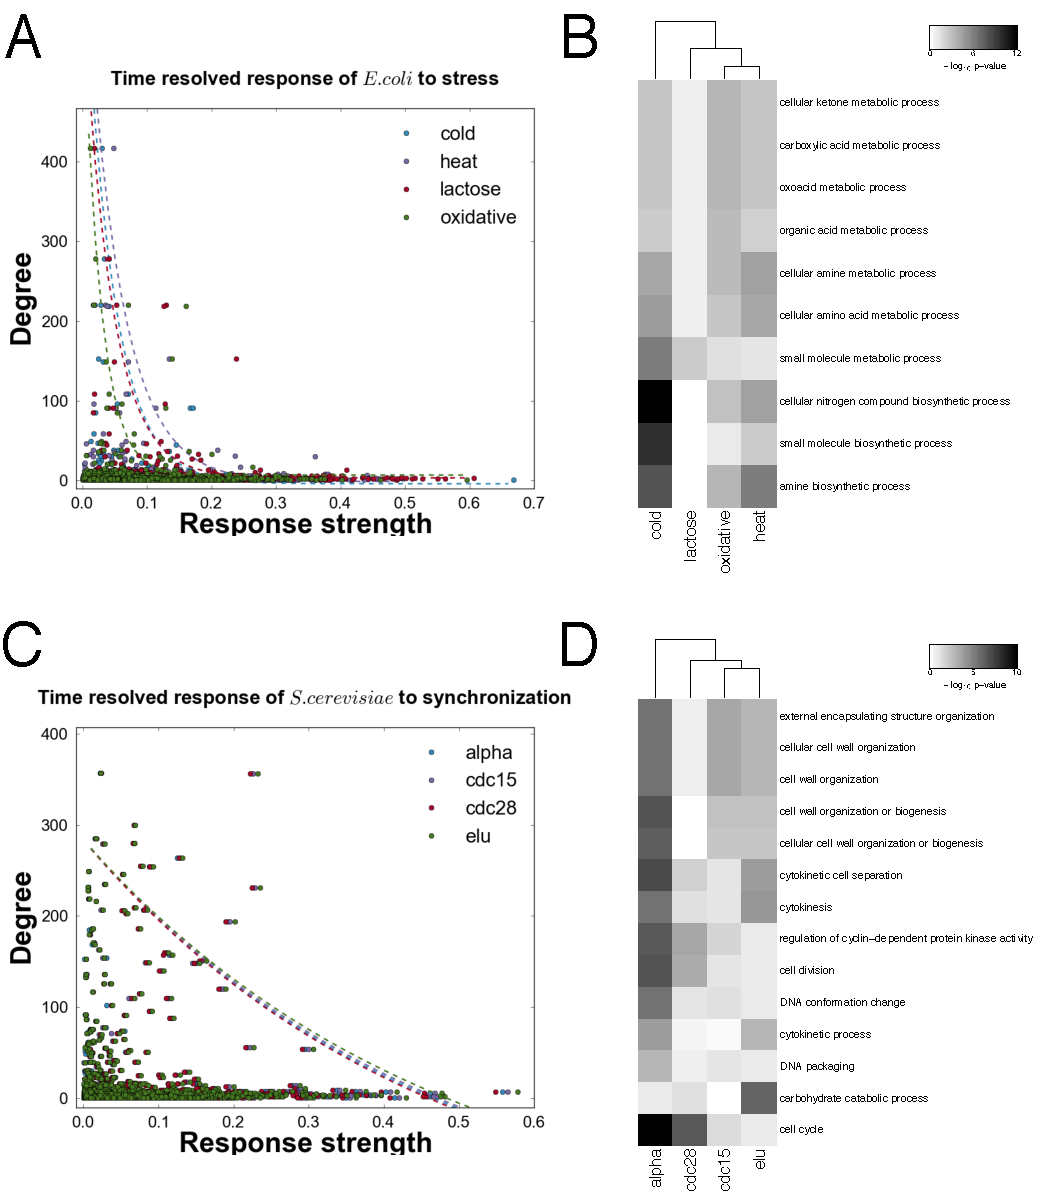
\includegraphics[width=\textwidth]{network/fig/ecoli_yeast_go.pdf}
\end{center}
\caption[GO term enrichment of strongly regulated genes]{
{\bf GO term enrichment of strongly regulated genes in the
\emph{E. coli} and yeast datasets.} 
}
\label{fig:response_qqplot}
\end{figure}

\section{Biological application}
We further went on to verify our hypothesis that strongly regulated peripheral 
genes are correlated with the phenotype by means of an \emph{in vitro}
mammalian cell system. Primary human keratinocytes extracted from the foreskin
migrate upon the treatment of hepatocyte growth factor (HGF), we measured
the gene expression profiles up to 8h after treatment of HGF (\citealp{Busch2008}) 
and identified
key genes with a large response strength according to MDS.

\subsection*{Invariant transcriptome response pattern}

%Cells coordinate their various functions as migration, proliferation or differentiation by regulation of their large gene interaction networks. To gain insight this gene network the usage of microarray analysis is nowadays state of the art. Time-dependent transcriptomic data are necessary to observe the dynamic response of cellular functions and decision. Fig.  (left panel) present the global gene response of different mammalian cells under diverse stimulation. The dynamic distributions of genes are ranked by the Multi-Dimensional Scaling (MDS) method (Figure 1, right panel). We quantify the relative dynamic response of all genes using a multi-dimensional scaling analysis (MDS). MDS embeds the high-dimensional distance matrix D of all pair-wise Euclidean distances between all gene expression kinetics into a low dimensional space, while conserving pair-wise distances \citealp{Strickert2009}.  Mapping the distance matrix $D$ onto a plane results in a cloud of points corresponding to the individual genes. Close or distant points represent genes with similar or dissimilar kinetics, respectively. We find the point cloud to be compact with few outliers, with the latter respresenting strongly responding genes having unique temporal expression profiles (Suppl. Fig. 7). 
Previous studies (\citep{Lu2007a,Mar2011}) have demonstrated a negative
correlation between the connectivity of a gene in the regulatory network
and its expression variance in the context of static disease models.
Here, we aim to address whether this negative correlation also exists 
between the network topology and its dynamic response.
In order to characterize the response strength over time of a certain gene, we
designed a metric based on multidimensional scaling (MDS). As a dimensionality 
reduction technique, MDS maps the high-dimensional gene expression profiles
to a low-dimensional space, while the relative pairwise distances are preserved
(\citealp{Taguchi2005,Tzeng2008}). Since genes with distinct kinetics have a
larger distance to the those with similar kinetics, and the dynamical behavior
is most likely a result of differential regulation, we created a metric to
describe the gene response strength based on its radial distance on the MDS
projection (Figure 1C right panel). In a real-world example where transcripts
are profiled in primary human keratinocytes under the stimulation of 
hepatocyte growth factor (HGF), we found the distribution of response
strengths has a long tail, indicating that 
only few genes are strongly induced by a certain stimulus, while the majority 
are barely regulated. Interestingly, this long-tail response strength
distribution is also observed in other cell types with various stimuli.
Among them are yeast cells that undergo cell cycles when synchronized by 
$\alpha$-factor, mouse skin cells stimulated with TPA and human Huh7.5 cells
under the stimulation of IFN-$\alpha$. It is known that the structures of
regulatory networks in various species are highly conserved 
(citation from Hauke), we thus hypothesize that this
universally invariant transcriptome response pattern results from the generic
topological features of the gene regulatory networks. Further questions 
arise, what distinguishes 
between the strongly and weakly responding genes? How is phenotype encoded 
in the gene network?

\subsection*{Topology is the determinant of dynamics in large networks}

To address the above questions, we applied biologically meaningful 
\emph{in silico} 
network models that are used to generate benchmark datasets for the DREAM 
(Dialogue for Reverse Engineering Assessments and Methods) challenge. The
model (\citealp{Marbach2010}) describes gene expression dynamics by the 
combinatorial regulation of upstream transcription factors. We constructed 
\emph{in silico} network models (Figure 2a) with a predefined topology from 
transcriptional regulatory networks in the \emph{E. coli} RegulonDB 
(\citealp{Gama-Castro2008}) 
and \emph{S. cerevisiae} (\citealp{Balaji2006}) or otherwise from a random,
uniform, scale-free or bow-tie network. Network dynamics was simulated after 
random 
multi-factorial perturbations from the steady state. Afterwards, the response 
strengths of individual genes are quantified by means of multidimensional 
scaling (Figure 2c). This workflow enables us to investigate how the dynamic
response pattern of a network relates to its topology. 

To first gain insight into the role that network topology plays, we compared
the different network responses after change of topology and change of kinetic 
parameters in an ensemble of \emph{E. coli} networks.
In the case of rewiring, we permutated the order of target nodes while keeping
the number of connections and kinetics parameters such as synthesis and 
degradation rates constant. Pearson correlation coefficients of the response
strengths before and after rewiring decrease slightly with the network size. 
In contrast, when we 
change the kinetic parameters without affecting the network topology (scheme, 
Figure 3A), the Pearson correlation coefficients remains at the same level and 
are in general higher than that before and after rewiring. The Kullback-Leibler
divergence, which measures the distance between two distributions, further 
confirms that the distance between the effect of rewiring and parameter change 
increases with the network size, indicating that network topology has a stronger 
impact on the response pattern, especially in large networks. 

\subsection*{Anti-correlation between connectivity and response}

To understand the functions of strong and moderate responders 
respectively, especially in a network point of view, we characterized
the relationship between the dynamic response of a node and its 
topological features with the help of an \emph{in silico} model of the
\emph{E. coli} network from RegulonDB. 
There is a weak but statistically significant
negative correlation between the degree of a gene and its response
strength. In other words, strong responders tend to have a low degree, 
whereas hub
genes with a high degree are hardly induced in general. We further characterized
the anti-correlation with a weighted exponential function, where the decay
constant $\lambda$ describes how strong this anti-correlation is.

With the help of the decay constant $\lambda$, we studied how the 
topology-response anti-correlation depends on the network structure.
While a hierarchically structured network, such as scale-free,
bow-tie networks, has a similar anti-correlation profile as the \emph{E. coli} 
network, random 
or uniform networks show a much higher variance in the anti-correlation between 
topology
and response. 

\subsection*{Strongly responding peripheral genes correlated with the phenotype}

The fact that strongly regulated genes always have a low degree and thus are
located at the periphery of the network poses the question whether these genes
mediate the computation of the whole network and then translate it into the 
phenotype. We therefore took the transcriptome data from the literature,
where time-resolved response of \emph{E. coli} (\citealp{Jozefczuk2010}) and 
\emph{S. cerevisiae} (\citealp{Spellman1998,Cho1998}) is 
measured under different stimuli. We found a similar anti-correlation between
network topology and response in the above datasets. Furthermore, we
carried out enrichment test of Gene Ontology (GO) terms in the significantly 
strong responders identified from MDS. For \emph{E. coli} cells in response
to different stress conditions, GO terms as metabolic processes, biosynthesis 
are over-represented in the strongly responding genes, which is in accordance
to the fact that cells have to adjust their growth rates under stress conditions.
On the other hand, for yeast cells in response to different synchronization
treatments, GO terms like cell wall organization, cytokinesis are more 
enriched than expected among strong responders, which is also in line with the
phenotype of cell cycles. Taken together, we found strongly induced genes, 
which are located at the periphery of gene regulatory networks, are nicely
correlated with the cellular phenotype.

\subsection*{Microarray datasets}

\section*{Figure Legends}

\paragraph*{Figure~1 }

Invariant transcriptome response patterns and the modelling approach. (A) 
Gene expression time series of primary human keratinocytes stimulated with 
hepatocyte growth factor (HGF). Histogram of the response strenth as determined by 
multidimensional scaling (MDS). (B) Histogram of the response strenth as determined by 
MDS for various cell types and stimuli. (C) Workflow to
investigate the relationship between topology and dynamics in a
thermodynamic model of cooperative gene regulation.
Time series are simulated after multi-factorial perturbations of the whole network.
MDS is applied to characterize dynamic response strengths
of individual genes.

\paragraph*{Figure~2 }

Effect of rewiring and parameter change on the network response 
pattern. (A) Schematic view of rewiring and the change of kinetic 
parameters, where black edges with a blunt head represent inhibiting
connections and red edges with an arrow head represent activating
connections, the values of kinetic parameters for each node are 
coded in gray scale. Dashed lines represent rewired edges. (B) Distribution 
of the correlation coefficients
before and after rewiring (change of parameters) in black (red) for 
different network sizes. (C) Kullback-Leibler divergence of the 
correlation coefficient distributions in B for different network
sizes.

\paragraph*{Figure~3 }

Correlation between the degree of a certain node in the network with its
response strength, which is defined by the radial distance in MDS.
Dashed lines are weighted exponential fits of the scatter plots from
1000 simulations with independent perturbations on the whole \emph{E. coli}
network from RegulonDB Version 6.2.

\paragraph*{Figure~4 }

Correlation between network dynamics and different topologies.
(A) Topology-respnose anti-correlation, as characterized by the decay constant 
$\lambda$, for different network structures. (B) Hierarchical clustering of 
different
network structures based on the Kullback-Leibler divergence between the $\lambda$
distributions.

\paragraph*{Figure~5 }

Strongly regulated peripheral genes are correlated with the phenotype.
(A) Topology-response anti-correlation of \emph{E. coli} in response 
to different stresses (extracted from \citealp{Jozefczuk2010}). (B) Topology-response
anti-correlation of \emph{S. cerevisiae} in response to different synchronizations
(extracted from \citealp{Spellman1998,Cho1998}). (C) Enrichment of GO terms
in the strongly induced peripheral genes of \emph{E. coli}. Shown are $p$-values
from Fisher's exact test in gray scale for different GO terms under different 
conditions. (D) Enrichment of GO
terms in the strongly induced peripheral genes of \emph{S. cerevisiae}. Shown 
are $p$-values
from Fisher's exact test in gray scale for different GO terms under different 
conditions.

\paragraph*{Figure~6 }



%\chapter{Signal flow}
\label{chap:flow}

From the previous chapter, we know that the cellular machinery of 
transcriptional and metabolic regulation is under-represented in the strongly 
regulated genes and thus hidden from the time-resolved transcriptome data. 
Consequently, the investigation of strong responders only gives insights into
the periphery of the gene regulatory network and functions directly related
to the cellular phenotype. What is largely missing is a holistic picture of
the signaling pathway activity, namely how the external stimulus is translated
to the protein signaling events that propagate through the protein interaction
network and ultimately lead to the measured gene regulation (\ref{fig:signal_flow}).

In the following, we first introduce several classical methods to infer the
enrichment of pathways from the transcriptome data. We point out the drawback
of their implicit assumptions and propose a two-step approach to identify the
causal signal\footnote{We use \emph{signal} and \emph{information} interchangably.} 
flow from membrane receptors to transcription factors. Finally,
we apply this approach in the study of cell-cell communication in the lung
cancer and skin.

\section{Pathway enrichment analyses}
Since the introduction of the microarray technology, pathway analysis has been 
a heavy focus and first choice for gaining insight into the underlying biology 
of differentially expressed genes. Over the past decade, we have seen at least 
three generations of pathway analyses~\citep{Khatri2012}, here we discuss 
their core features and limitations.

\subsection{Over-representation test}
Over-representation test is also called Fisher's exact test, it statistically 
evaluates the fraction of genes in a particular pathway found among the set 
of genes showing significant changes in expression. By constructing a
$2 \times 2$ contingency table, a researcher first chooses genes that are 
differentially over- or under-expressed in a given condition at a certain 
threshold. Then, for each pathway, the number of genes that are part of the 
pathway is counted. This process is repeated for an appropriate background 
list of genes (e.g., all genes measured on a microarray). Next, every pathway 
is tested for over- or under-representation based on this contingency table. 
The most commonly used test is based on the hypergeometric distribution or
the Fisher's exact test.

One of the critics on Fisher's exact test is that it only considers a ranked
list of differentially expressed genes and is thus independent of the 
measured fold changes. Second, the generation of the contingency table
requires setting a significance cutoff to count the number of differentially
regulated genes. This procedure introduces a subjective criterion and 
effectively treats the gene regulation as a black-white picture, namely only 
genes above this threshold are considered differentially expressed and those
below the threshold are then discarded.
    
\subsection{Gene set analysis}
To avoid the arbitrary significance cutoff and to realize the fact that weaker 
but coordinated changes in sets of functionally related genes (i.e., pathways) 
can also have significant effects, gene set enrichment analysis was suggested~%
\citep{Subramanian2005,Luo2009}. In general,
a pathway-level (gene group level) statistic is calculated from the gene-level 
statistic, and the statistical significance is assessed according to the 
pathway-level statistic.

By considering the coordinated changes in gene expression, gene set analyses 
account for dependence between genes in a certain pathway or group, however,
each pathway is still analyzed independently and thus crosstalks between
pathways are disregarded.

\subsection{Topology-based approach (SPIA)}
Over-representation and gene set analyses only consider the number of genes 
in a pathway to identify significant pathways, and ignore the additional 
information available from various prior knowledge bases. Recently a signaling
pathway impact analysis (SPIA) was proposed~%
\citep{Tarca2009}. SPIA considers the structure and dynamics of an entire 
pathway by incorporating changes in gene expression, types of interactions, 
and the positions of genes in a pathway. 
It calculates the pathway-level statistic from the combinatorial probability 
of perturbation in gene expression and over-representation. One obvious problem 
of the topology-based approach is that the true pathway topology is highly
context-dependent and remains poorly understood and annotated.

\subsection{NetSearch}
\cite{Steffen2002} further built upon the idea of incorporating 
prior knowledge about the pathway topology and suggested
the inference of signal transduction networks with protein-interaction maps
and expression profiles from DNA microarrays.
It works by first enumerating all possible linear paths
of a specified length through the interaction map starting
at any membrane protein and ending on any DNA-binding
transcription factors.
Microarray expression data are then used
to rank all paths according to the degree of similarity in
the expression profiles of pathway members.
Linear pathways
that have common starting points and endpoints
and of the highest ranks are then combined into the final
model of the branched networks.

Based on the gene expression data of pheromone response in the yeast, the 
NetSearch algorithm accurately reconstructs the MAPK cascade, it also identifies a 
network with other proteins necessary to execute the coordinated processes of 
growth polarization and cell cycle arrest, and reflects the complex topology of 
the interaction network in response to pheromone.

\subsection{Drawback}
All the above methods make the implicit assumption that the expression of genes
and their corresponding protein products are correlated, or the signaling 
pathway activity, which is largely determined by the member protein level, 
can be inferred from the transcriptome data. There has been ongoing debate 
about whether the transcriptome regulation correlates with the proteome
in bacterial and mammalian cells~\citep{Taniguchi2010,Ghazalpour2011}. 

More
often than not, the assumption of correlation either does not hold or strongly depends on the context~\citep{Soufi2009}. 
It has also been shown that the mRNA-protein expression correlation increases 
with time~\citep{Fournier2010}.
As one of the protein classes important in disease, 
transcription factors (TF) remain largely decoupled at the 
protein
and mRNA level. Many of the TFs that regulate physiological
    targets are constitutively present, and their activity is determined
    by posttranslational modifications such as phosphorylation%
    ~\citep{Messina2004}.
Therefore, questions arise about the validity of inferring signaling 
pathway activity based solely on the gene expression level.

\section{Two-step integrative approach to causal signal flow}
We propose here a two-step integrative approach to infer the activated protein signaling
pathways from time-resolved microarray data. As a first step, we apply a
gene set enrichemnt analysis to test the
enrichment of transcription factor target genes, which acts as a proxy of
the transcription factor activity \emph{per se}. Second, the upstream 
signal flow from membrane receptors to transcription factors is predicted 
based on the distance between both end nodes in the protein interaction
network.

\subsection{Identification of activated transcription factors}
We performed gene set enrichment tests, 
using a modified implementation~\citep{Luo2009}.
To this end, we retrieved sets of genes regulated by 
a common transcription factor from MSigDB v3.0 (The Molecular Signature Database, \cite{Liberzon2011}). 
This database contains two major data sources. The first one is mammalian 
transcriptional regulatory motifs from the v7.4 public version of TRANSFAC 
database~\citep{Matys2003b}. We then generated the motif gene sets consisting 
of the inferred target genes for each motif. Every such set consists of human 
genes whose promoters (defined as regions -2kb to +2kb around transcription 
start site) contain at least one instance of the motif.
The second data source for transcription factor targets in MSigDB is derived 
from upstream motifs highly conserved among five mammalian species~%
\citep{Xie2005e}. Each motif gene set consists of all human genes whose 
promoters contained at least one conserved instance of the motif.

Individual genes were  ranked according to their response strengths as derived from the 
multidimensional scaling of the normalized time series 
(\ref{sec:response_strength}). 
The gene sets from MSigDB were  then tested for their enrichment 
 relative to the whole transcriptome by a Kolmogorov-Smirnov statistic. 

\subsection{Signal flow from membrane receptors}
In order to infer how extracellular signal flows from the membrane receptors to 
the transcription factors and subsequently induces gene regulation, it is 
crucial to be able to measure the proximity between a given pair of receptor and
transcription factor in the protein-protein interaction network. Here we 
compare two distance metrics, one is the shortest path length, and the other
being the mean first passage time based on the idea of random walk.

\subsubsection{Shortest path length}
If one assumes that information propagates in the network in a most parsimonious
or efficient way,
shortest path (SP) length between two nodes in the network is a classical way to
assess the distance between these two nodes and thus possible route of signal flow
(\ref{sec:shortest_path}). Several variations of the 
shortest path approach have been used in extracting 
phenotype associated and previously unknown genes~%
\citep{Zhou2002,Managbanag2008}.

When multiple target genes exist, the well-known graph-theoretical concept of a Steiner tree is often used in place of a set of shortest paths. Given a set of nodes to be connected, a Steiner tree is an acyclic subgraph (a tree) connecting all these nodes while using the minimum number of edges. In a Steiner tree, the individual path from the putative causal gene (the root of the tree) to each of the target genes does not need to be the shortest, but the size (i.e., the number of edges) of the whole tree is minimized. The Steiner tree approach has been used to find new functional associations for proteins~\citep{Huang2009,Bailly-Bechet2011}.

We use a directed human protein-protein interaction network from a previous study
\citep{Vinayagam2011}, which contains edge directions
inferred by a naive Bayesian classifier.
For each cytokine receptor/transcription factor pair previously identified,
we calculated the length of the shortest path between the two
using the unweighted breadth-first search algorithm,
as implemented in the R package \texttt{igraph}~\citep{Csardi2006}.
We use these lengths as base metric for the probability 
of signal actually flowing through the pathway.

Intuitively, the shortest path is only the best scenario of all possible routes
of information flow in the network. Therefore, it simply ignores the 
neighborhood or global structure around the shortest path when calculating
distances. Another limitation of the shortest path distance metric has to do
with the small characteristic path lengths in a small-world networks~%
\citep{Watts1998}, such that any nodes can be reached from any other nodes
within only few hops when traveling on the shortest path and the shortest path
metric loses its discriminative power. Since most biological
and real-world networks demonstrate the small-world feature~%
\citep{Barabasi2004}, this limitation
has to be kept in mind when working with the shortest path.

\subsubsection{Mean first passage time}
Another category of distance metric in networks is the 
so-called flow-based methods, which compute the fraction of flow going through each intermediate node/edge. In the case of current flow approach, the network is modeled to mimic the behavior of current in an electronic circuit, where each edge has an associated resistance~\citep{Missiuro2009}. The current flow approach is
also shown to be equivalent to a random walk in the network~%
\citep{Doyle2000}.

The mean first passage time (MFPT) is defined as the average time/steps 
necessary for 
a random walker starting from a source node to reach a target node for the
first time. It has been shown that MFPT can be used to detect community
structures in the protein interaction network of yeast~\citep{Zhou2003}. 
Recently, a random walk with restart approach was applied to associate
target gene sets to reference datasets as an alternative to 
over-representation-based enrichement analyses~\citep{Glaab2012}. 
Further examples include a random walk-based software tool for functional
analyses of cellular networks with genomic data integrated~\citep{Komurov2012a}.
Moreover,
the usefulness of MFPT became evident by the fact that the pairwise MFPT 
matrix is sufficient to reconstruct the full network topology~%
\citep{Wittmann2009}.

MFPT can be calculated analytically by solving a linear equation system~%
\citep{Kampen2007}. Consider the special case of a linear chain 
(\ref{fig:mfpt_calculation}) and suppose the random walker starts from node 
$x$ at a certain time $t$, with the probability of jumping to adjacent nodes
being equal, we have
\begin{equation}
\tau(x,y) - 1 = \frac{1}{2}\tau(x-1,y) + \frac{1}{2}\tau(x+1,y)
\label{eq:mfpt}
\end{equation}
where $\tau(x,y)$ denotes the mean first passage time of reaching $y$ and 
starting at $x$, which can be decomposed of 1 time unit needed to reach the
next time step $t+1$ and the travel time to the target node $y$ at $t+1$.
Since the random walker can be at either node $x-1$ or $x+1$ at $t+1$, each
with equal probability, we express the mean first passage time to $y$ at
time step $t+1$ as the right-hand-side of \ref{eq:mfpt}.

\begin{figure}[!ht]
\begin{center}
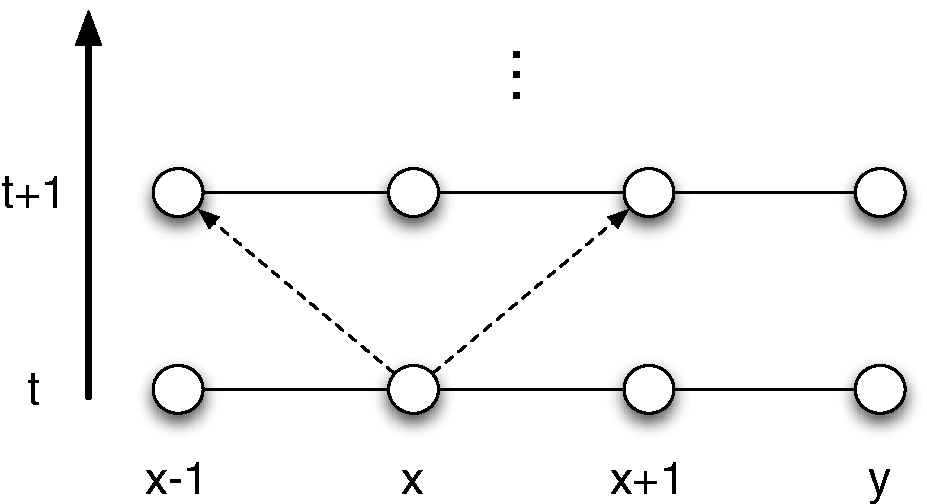
\includegraphics[width=0.8\textwidth]{mfpt_calculation.pdf}
\end{center}
\caption[MFPT calculation]{
{\bf The calculation of MFPT on a linear chain.}
The same linear chain consisting of 4 nodes is depicted in different time 
slices ($t,t+1,\ldots$), 
a random walker starting from node $x$ at time $t$ can jump to either $x-1$ 
or $x+1$ at time $t+1$.
}
\label{fig:mfpt_calculation}
\end{figure}

\ref{eq:mfpt} can be rewritten and generalized to an arbitrary graph, i.e.
the mean first passage time from all possible nodes to a target node $y$
can be expressed as a linear equation system
\begin{equation}
(\tilde{\mathbf{L}}-\boldsymbol{\beta}^y) 
\begin{pmatrix}
\tau(1,y)\\
\tau(2,y)\\
\vdots\\
\tau(N,y)
\end{pmatrix}
= \boldsymbol{\delta}
\label{eq:mfpt_system}
\end{equation}
where 
\begin{equation}
\delta_i=
\begin{cases}
0 & i=y\\
1 & \textnormal{otherwise}
\end{cases}
\end{equation}
and $\tilde{\mathbf{L}}$ is the normalized graph Laplacian and
\begin{equation}
\tilde{L}_{ij}=
\begin{cases}
1 & i=j\\
-1/deg(i) & i \neq j \ \textnormal{and}\ i \ \textnormal{is adjacent to}\ j \\
0 & \textnormal{otherwise}
\end{cases}
\end{equation}
where $deg(i)$ is the degree of node $i$. $\boldsymbol{\beta^y}$ 
is the boundary condition
matrix that ensures $\tau(y,y)=0$, more specifically
\begin{equation}
\beta^y_{ij}=
\begin{cases}
\tilde{L}_{ij}-1 & i=j=y\\
\tilde{L}_{ij} & i=y\\
0 & \textnormal{otherwise}
\end{cases}
\end{equation}
It is easy to see that $\tilde{\mathbf{L}}$ can be pre-calculated and then be 
reused to estimate the
MFPT for each target node $y$. Moreover, the calculations
for different targets are independent and hence can be
determined in parallel. As networks in biology are often
sparse, the equation system in \ref{eq:mfpt_system}
is suitably represented by a sparse matrix. The matrix
is positive semi-definite and can be solved by the LGMRES algorithm~%
\citep{Baker2005}.

\ref{fig:mfpt_toy} compares the distance measure of shortest path (SP) length
and mean first passage time (MFPT) on different toy networks. Network A, B and
C are all composed of a linear chains as the backbone and different complex 
global structures, the SP metric measures the length of the backbond and is 
thus the same across all three topologies, whereas MFPT has a broader range
and changes between 9 and 17.5. This demonstrates that SP does not take into
account the global network topology. Furthermore, SP is also more susceptible
than MFPT to the pruning of a critical link, which is illustrated in the 
network C and D with only a single connection between $n1$ and $n2$ removed
in D. Since this edge is part of the shortest path between $n0$ and $n3$, the
SP distance changes dramatically by 33\%, while MFPT increase only moderately
by 3\%.

\begin{figure}[!ht]
\begin{center}
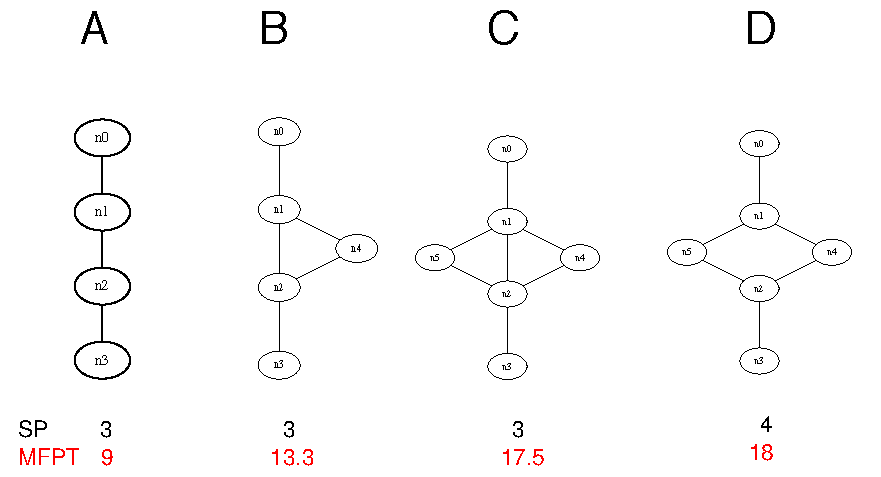
\includegraphics[width=\textwidth]{mfpt_toy.pdf}
\end{center}
\caption[Toy example of SP and MFPT on different topologies]{
{\bf Comparison of shortest path (SP) length and mean first passage time 
(MFPT) on different toy networks.}
Shown are the distances between node $n0$ and $n3$ measured in shortest path 
(SP) and mean first passage time (MFPT) respectively.
}
\label{fig:mfpt_toy}
\end{figure}

\section{Application in tumor-stroma interaction of lung cancer}

The hallmark of lung tumor development is its early spread, 
complicating the patient treatment and strongly impairing survival.
Recent studies have shown the tumor-stroma interaction to be relevant to 
tumor growth and spread, and therefore a possible target for
novel, effective treatment. 
However, 
the details by which tumor and stroma cells communicate remain poorly 
understood. In this section we present a study
of the migration mechanisms of a non-small-cell lung 
tumor cell line (H838) under the influence of endothelial (HPAEC) cells 
in a coculture system.

To obtain a holistic overview of the migratory processes, 
we recorded the time-resolved changes in the transcriptome of tumor cells
in scratch assays of aforementioned cocultures, and measured
cytokine concentrations in the medium.
H838 showed a significantly increased migration area after 24h in the 
H838/HPAEC coculture compared to the H838/H838 coculture.
Two cytokines, TNF-$\alpha$ and SDF-1$\alpha$, were shown to directly 
induce migration, 
and the transcripts of these two key factors were regulated only 
in HPAEC cells.
Gene set enrichment test identified coordinated regulation
of transcription factors targets
that cause the transcriptome response in H838. 
We compared distances from the cytokine receptors to the predicted
transcription factors using both shortest path and mean first passage time.
%suggests that TNF-$\alpha$ receptors activate multiple
%downstream targets in a homogeneous fashion,
%whereas the shortest paths \change[JB]{between}{descending from} 
%the SDF-1$\alpha$ receptor
%have multiple characteristic path lengths. 
%We conclude that TNF-$\alpha$ induces \change[JB]{the sustained}{an unspecific} 
%activation 
%of various downstream transcription factors, 
%which is the \change[JB]{primary}{initial} response \remove[JB]{mechanism} 
%involved in the 
%migration of H838 cells. 
%At the same time, the delayed activation of SDF-1$\alpha$ induce\change[JB]{d}{s 
%specific} pathways 
%\add[JB]{that} could provide a fail-safe mechanism.

\subsection{Background}
Lung cancer with its predominant type non small cell lung carcinoma 
(NSCLC) is the leading cause of cancer-related mortality worldwide.
The hallmark of lung cancer is its early spread, 
making it particularly dangerous, with associated high rate of death 
and short survival.
Whether this is an inherent feature of the non-small cell 
lung tumor cells or 
due to their microenvironment is still unknown. 

Ever since the formulation of \emph{seed and soil} theory by the English 
surgeon Stephen Paget in 1889~\citep{Paget1889}, there has been increasing 
interest in studying the tumor-stroma interactions. 
It is now largely acknowledged that sites of metastasis are determined 
not only by the characteristics of the tumor
cells but also by the microenvironment of
the host tissue~\citep{Fidler2003}. Tumor cells can generate a supportive
microenvironment by producing stroma-modulating
growth factors, which act in a
paracrine manner to induce stromal reactions such as
angiogenesis~\citep{Bergers2003}
and inflammatory response~\citep{Coussens2002}. Stroma cells in turn can
interact with primary tumor cells synergistically and facilitate their migration~%
\citep{Wyckoff2004}.
Stromal cells also make promising drug targets, since they are not as 
genetically
unstable as cancer cells, and are therefore less likely to
develop drug resistance~\citep{Kerbel1997}. To date, a number of drugs targeted
at tumor microenvironment, i.e. endothelial cells, immune cells and components
of the extracellular matrix, are at different stages of clinical 
trials~\citep{Mueller2004}. However, side effects of such stroma-targeting drugs
have also been observed, which raises the natural demand of a more detailed, 
systematic understanding of the tumor-stroma interaction.

While bearing in mind that tumor-stroma interactions can be mediated by direct cell-cell contact or modification of the extracellular matrix
components~\citep{Micke2004a}, most studies have focused on the tumor-stroma interaction through
single soluble factors~\citep{Kryczek2007,Saijo2002i,Nakamura1997}. 
\cite{Zhong2008} identified cytokines that are crucial for the 
tumor cell proliferation
and stromal cell migration by screening the whole secretome from
an adenocarcinoma/stromal murine lung cell coculture.
\cite{Sato2004} studied
the transcriptome homeostasis of pancreatic
cancer cells and stromal fibroblasts,
and singled out candidate genes that are
differentially expressed in coculture.
One of the most important types of stromal cells are endothelial cells (EC), 
the integral components of blood vessels. ECs not only promote the homeostasis of 
vascular system, but play an important role in tumor progression as well. 
It was shown that ECs influence different responses of cancer cells, such as 
proliferation and invasiveness \emph{in vitro}, as well as the metastatic potential 
of tumor cells \emph{in vivo}~\citep{Franses2011}.

Here, we combine the previous approaches and
study \emph{in vitro} the crosstalk between tumor and 
endothelial cells in  a non-small-cell lung cancer model: namely,
H838 lung cancer cells and HPAEC, i.e. human pulmonary artery endothelial cells.
We found that the  migration of  H838 cells in a trans-well H838/HPAEC coculture
was significantly enhanced when compared to monoculture.
Gene set enrichment analysis of the dynamic transcriptome
response of the H838 cells  revealed a coculture specific response 
that correlated with enhanced migration.
A cytokine array and subsequent single factor stimulation
identified the cytokines \tnfa and \sdfonea
to be the main factors enhancing H838 cell migration,
being \emph{de novo} expressed and originating in the endothelial cells alone. 

We further 
traced causes of the transcriptome response in the tumor cells back to the
\tnfa and \sdfonea receptors. % via the transcription factors and upstream protein signaling.
%We identified the dynamic regulation pattern of transcription factors. 
Assuming that cellular signal is most likely transmitted through the shortest 
path in a protein-protein interaction network, we 
mapped the putative pathways linking cytokine receptors with the 
transcription factors evoking the transcriptome response. 
%Based on \change[JB]{the above}{our results}, we hypothesize that \tnfa receptor family 
%members are likely associated with a wide spectrum of transcription factors, which
%renders the \tnfa-induced pathway an unspecific response in the first place.
%On the other hand, the \sdfonea receptor CXCR4 
%preferentially activates transcription factors such as 
%STAT3/6, LMO2, HSF1, IRF2, JUN/FOS, which are predominantly 
%enriched between 12 and 16 hours after coculture and represents a fine-tuned
%secondary activity leading to migration. \note[SD]{Should we mention the purpose of the paper in few sentences?}

% We need some concluding sentence here wraping up teh biology


% Results and Discussion can be combined.
\subsection{Results}

\subsubsection{H838 migration rate is enhanced in a transfilter co-culture with HPAEC cells}

To investigate the changes in migration behavior of lung tumor cells under the 
influence of stromal cells we cultivated  
H838 cells  together with either human pulmonary artery endothelial cells (HPAEC) or additional H838 cells in a trans-filter system (\ref{fig:migration} A).
The experimental setup (\ref{fig:h838_setup}) of the homo- and heterogeneous cocultures ensured 
similar physical and environmental conditions, thereby minimizing 
experimental artifacts, e.g. due to different cell numbers per conditions. 

Tumor cells on the bottom of the cell culture dish were scratched and the 
closing of the cell-free area was observed using time-lapse microscopy, in both
homo- and heterogenous cocultures (\ref{fig:migration} B).
In the heterogeneous cocultures, 
H838 cells close on average $963.5\pm156.8\ \mu m^2$ 
(mean $\pm$ standard deviation) within 24h, 
against $702.8\pm104.0\ \mu m^2$ in the homogeneous cocultures 
(\ref{fig:migration} C). 
% Note that we should put all these figures into one panel 
The migration area of the heterogeneous cocultures is significantly higher, and
a two-sided  $t$-test of the difference observed yields a $p$-value of 
$2.82 \times 10^{-5}$.

\begin{center}
\captionsetup{labelformat=prepage}
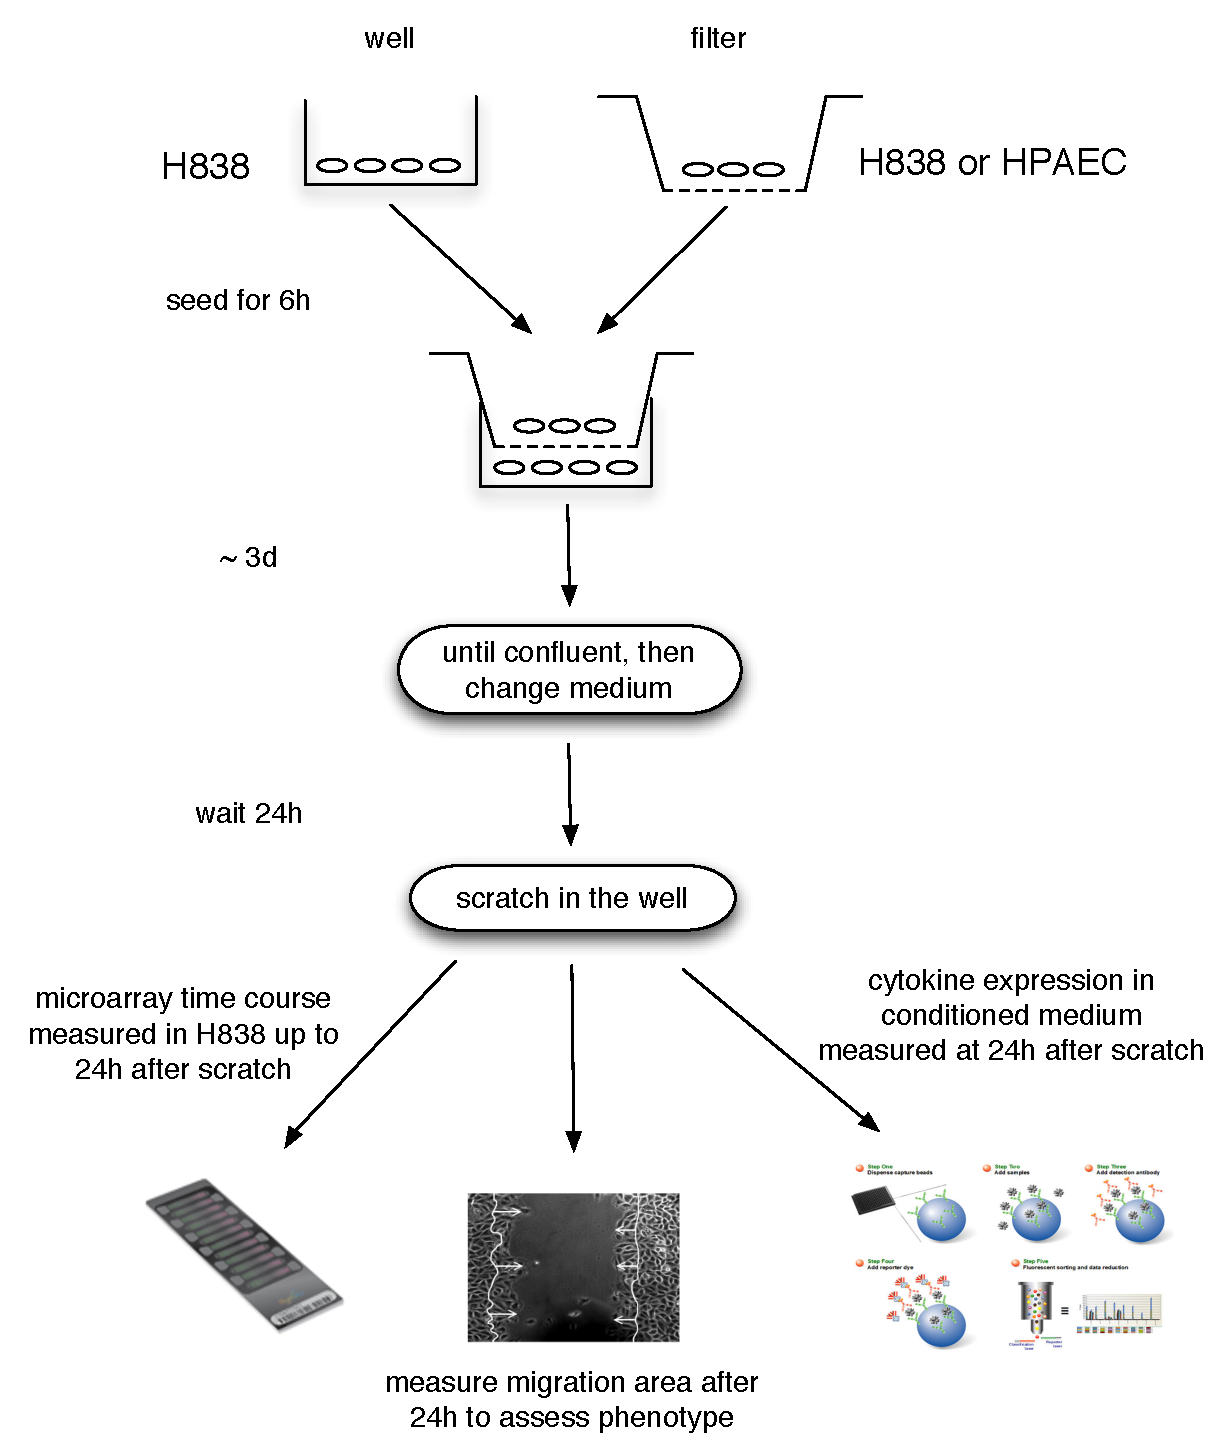
\includegraphics[width=\textwidth]{h838_setup.pdf}
\newpage
%\begin{FPfigure}[!ht]
\captionof{figure}[H838 experimental setup]{
{\bf The experimental setup of the tumor-stroma interaction 
between H838 and HPAEC cells.} 
The coculture of tumor and endothelial cells is carried out
in a trans-filter system, where the lung cancer cell line
H838 is cultivated in a well and on top of that is a filter
with either the same tumor cells or the endothelial cell
line HPAEC. Both cell types are seeded for 6 hours before 
the well and the filter are brought together. After 
approximately 3 days of coculture and both the well and the 
filter layers become confluent, medium is changed. Then
after another 24 hours, multiple scratches are performed
in the bottom well. Migration phenotype is measured within
24 hours after scratch and the cell and supernatant samples 
are subject to the transcript and cytokine profiling 
experiments respectively.
}
\label{fig:h838_setup}
%\end{FPfigure}
\end{center}

\begin{figure}[!ht]
\begin{center}
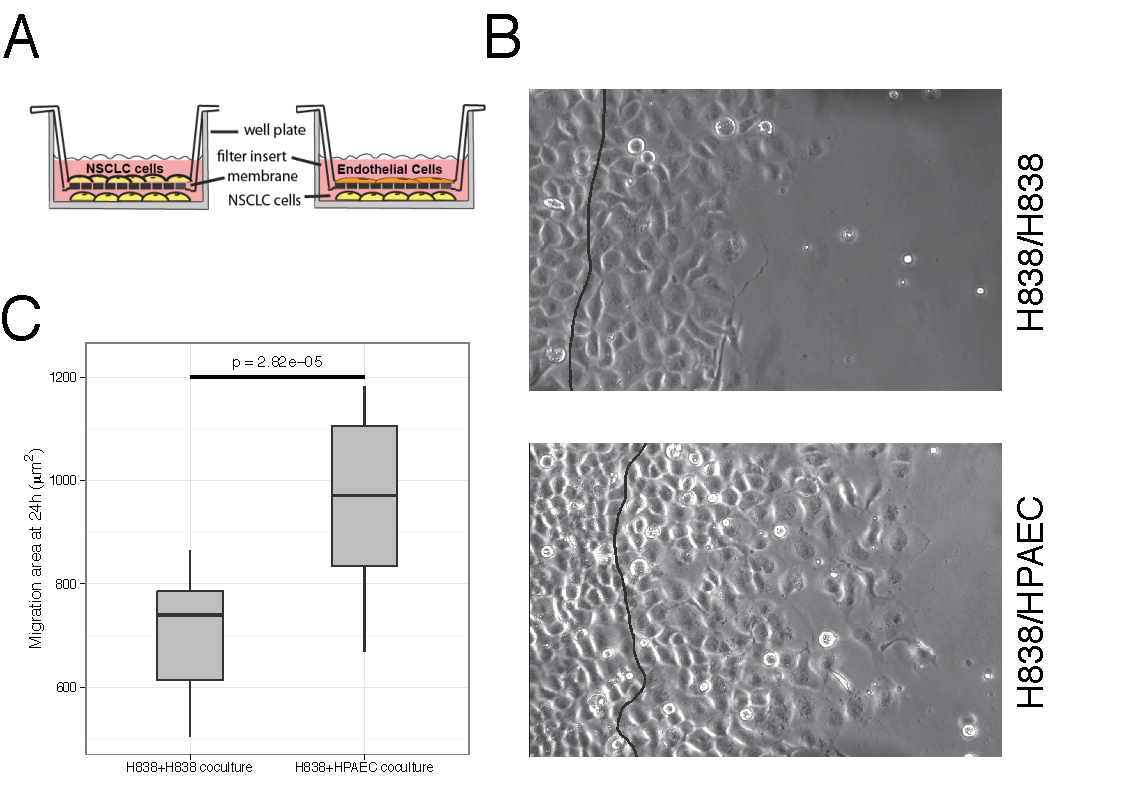
\includegraphics[width=\textwidth]{fig-migration.pdf}
\end{center}
\caption[H838 migration in homo- and heterogeneous coculture]{
{\bf Migration of H838 cells in the homo- and heterogeneous coculture.} 
(A) Trans-filter system. (B) Scratch assay of the homo- and heterogeneous coculture.
(C) Migration area of H838 cells at 24h after scratch from multiple independent 
experiments 
plotted as 
boxplots for the homogeneous (H838 + H838) and heterogeneous (H838 + HPAEC) 
coculture.
}
\label{fig:migration}
\end{figure}

The \emph{in vitro} scratch assay is a well established method
to study cell migration~\citep{Busch2008,Liang2007}, especially
in our experimental setting, the coculture of tumor and 
endothelial cells has no influence on the cell proliferation~%
\citep{Dauscher2012} and thus our results can be interpreted
as the net effect of tumor cell migration.

\subsubsection{Transcriptome response of H838 cells}
To explore the mechanisms leading to the enhanced cell migration, we recorded the time-resolved transcriptome response of the tumor cells during migration.
Illumina Human HT-12 Expression BeadChip was employed to compare the dynamic transcriptome response of scratched H838 cells in both homo- and heterogenous coculture conditions.
We collected mRNA at $t=(0,0.5,1,2,3,4,5,10,15,24)h$ after scratching for microarrays,
the data of which were quantile-normalized~\citep{Dunning2008a}.  
Discarding lowly expressed probesets and those with low interquartile 
variability between samples, we finally mapped the probes to 14922 EntrezID 
annotated genes. 
% Here we should show a time-resolved GO analysis or something similar (Fig. 2)
% Also add the analysis in the materials and methods

We analyzed the basal differential gene expression between homo- and
heterogeneous coculture by linear model fitting and Bayesian variance estimation~%
\citep{Smyth2004}, as well as the dynamic differential gene expression by fitting
the time series with a full/reduced polynomial model~\citep{Mar2009}. At 0h, only 2
genes are significantly down-regulated (Benjamini-Hochberg
corrected $p$-value $<0.01$) in the homogeneous coculture with respect
to the heterogeneous coculture 
(\ref{fig:h838_transcriptome} A). Over time, there are more
genes classified as significantly up- and down-regulated by comparing the full and
reduced model fitting (\ref{fig:h838_transcriptome} B). 
We further looked at the time course of all genes that are
significantly ($q<0.01$) regulated over time from 
\ref{fig:h838_transcriptome} B. In the heterogeneous
coculture of H838 and HPAEC cells, most genes are 
moderately up-regulated over time, with the maximal
log fold expression being 1.25 relative to 0h.
Taken together, the majority of genes
in H838 cells are not differentially expressed in the homo- and heterogeneous
coculture conditions. We hypothesize that those 
differentially regulated genes do undergo certain specific
phenotypic transformations, but the response of the H838
transcriptome to heterogeneous coculture is rather weak.

\begin{figure}[!ht]
\hskip 0.5in A \hskip 2.5in B
\begin{center}
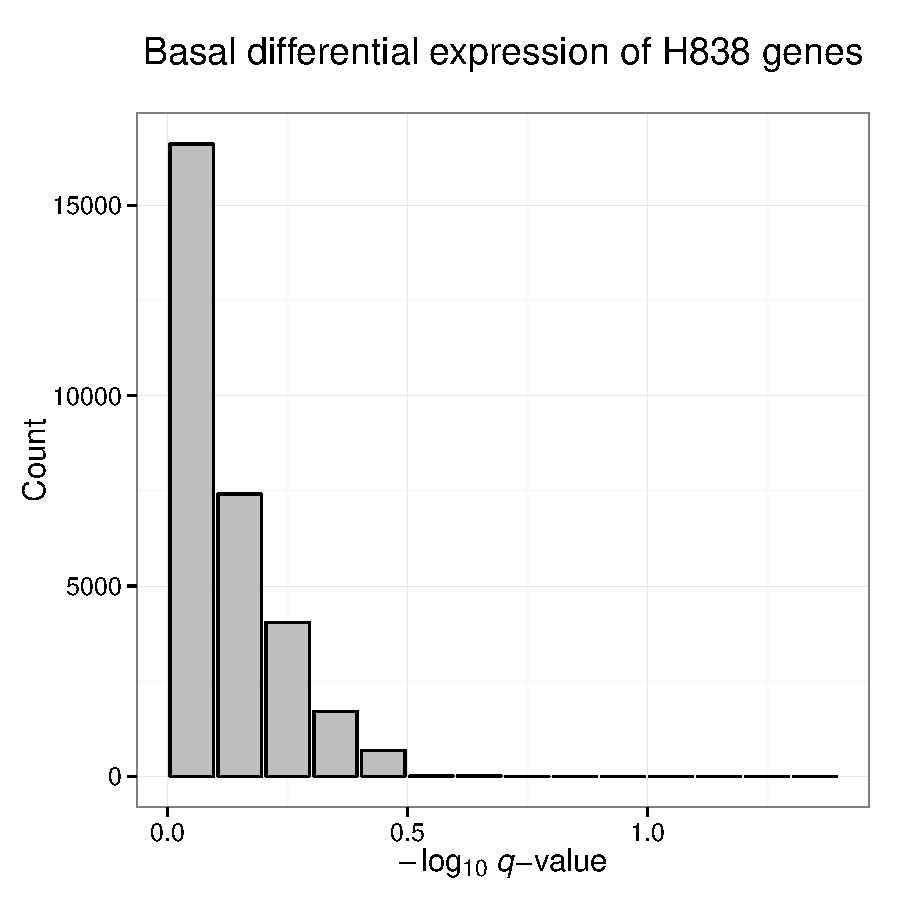
\includegraphics[width=0.45\textwidth]{h838-basal_hist.pdf}
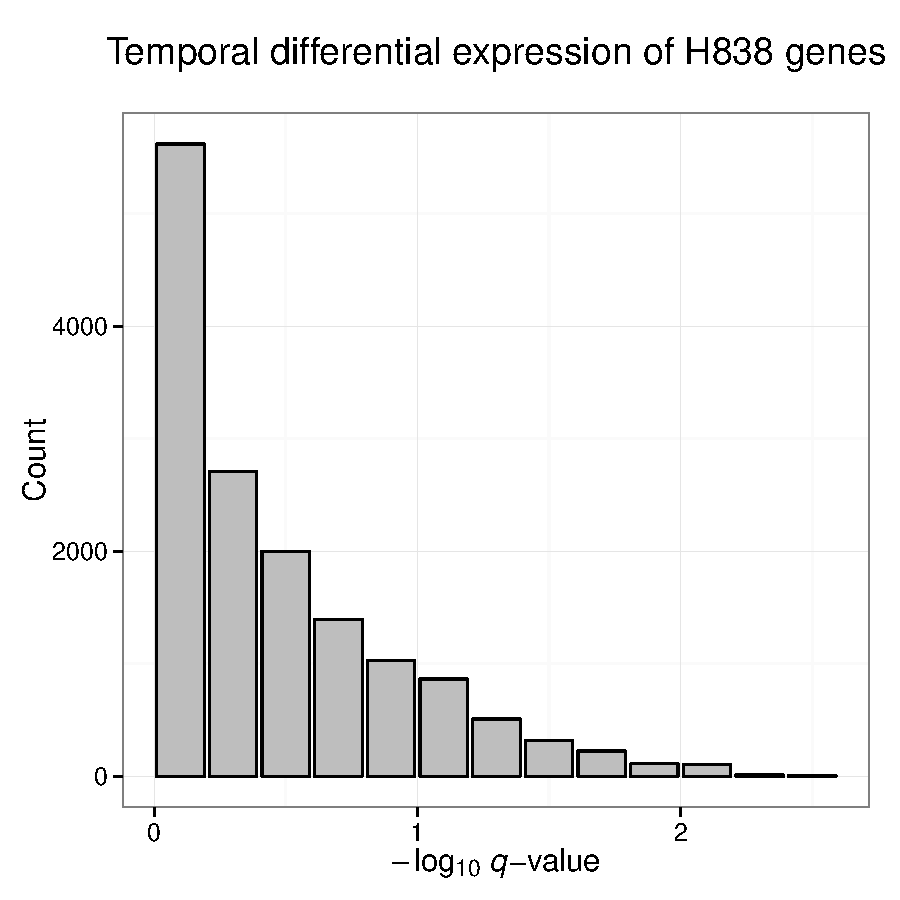
\includegraphics[width=0.45\textwidth]{h838-fit_hist.pdf}
\end{center}
\caption[Differential basal and dynamic gene expression]{
{\bf Differential basal and dynamic gene expression in homo- and heterogeneous 
cocultures.} 
(A) Histogram of the differential gene expression at 0h as determined by limma~%
\citep{Smyth2004}. 
Basal differential expression is 
represented as the negative log-transformed and multiple
testing corrected $p$-value of the limma test.
(B) Histogram of the differential gene expression over time as determined by the
full/reduced model fitting~\citep{Mar2009}.
Dynamical differential expression is 
represented as the negative log-transformed and multiple
testing corrected $p$-value of the full/reduced model
likelihood ratio test.
}
\label{fig:h838_transcriptome}
\end{figure}

\begin{figure}[!ht]
\begin{center}
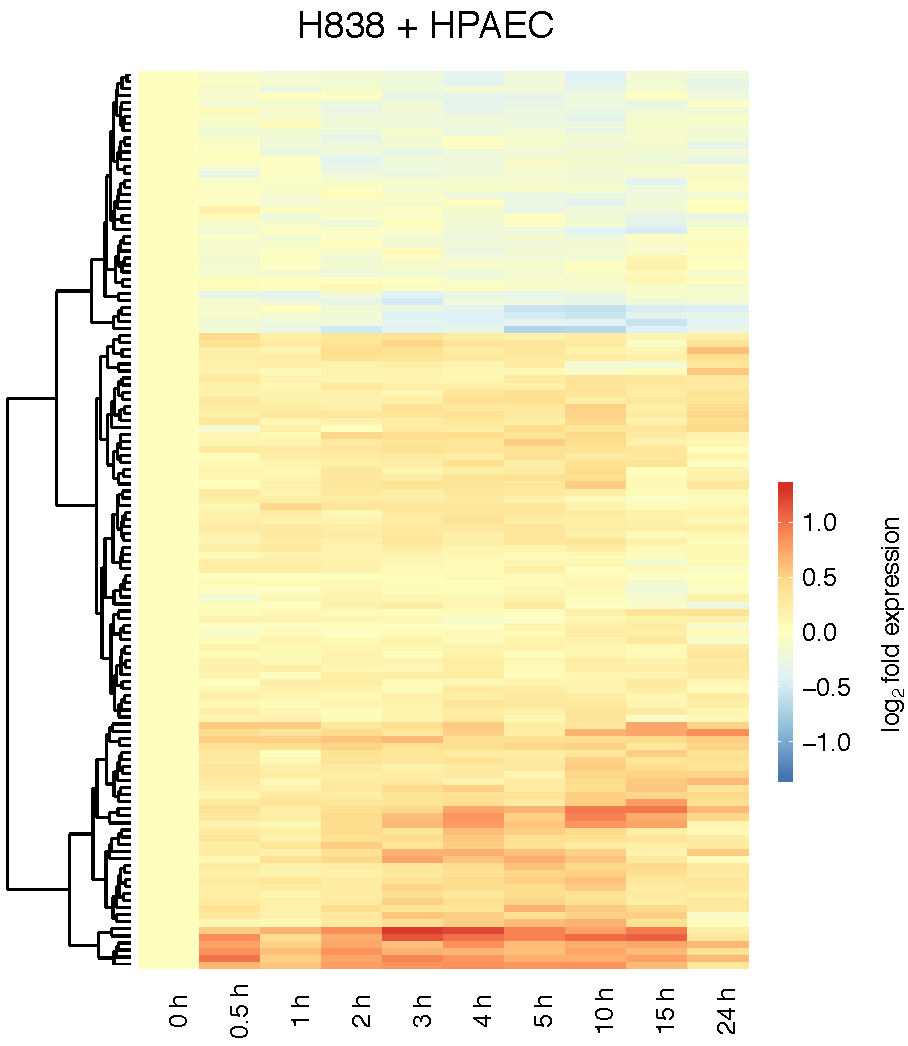
\includegraphics[width=\textwidth]{h838_ts_heatmap.pdf}
\end{center}
\caption[H838 migration in homo- and heterogeneous coculture]{
{\bf Migration of H838 cells in the homo- and heterogeneous coculture.} 
(A) Trans-filter system. (B) Scratch assay of the homo- and heterogeneous coculture.
(C) Migration area of H838 cells at 24h after scratch from multiple independent 
experiments 
plotted as 
boxplots for the homogeneous (H838 + H838) and heterogeneous (H838 + HPAEC) 
coculture.
}
\label{fig:h838_ts}
\end{figure}

In order to take a glance at what is the function of those
differentially regulated genes, and to overcome the difficulty in detecting weak
but simultaneous regulation, we analyzed the transcriptome data with gene set
enrichment test~\citep{Luo2009}.
The comparison between heteregeneous and homogeneous coculture yields 
a mixture of experimentally determined gene sets, both for the basal level
(\ref{fig:h838_basal_gage_msigdb})
and the differential expression over time (\ref{fig:h838_dynamic_gage_msigdb}).
In other words, the H838 cells in the heteregeneous and homogeneous coculture
do not tend to have a qualitatively different phenotype and are migrating in
both cases as is also observed in the scratch assay.

\begin{figure}[!ht]
\begin{center}
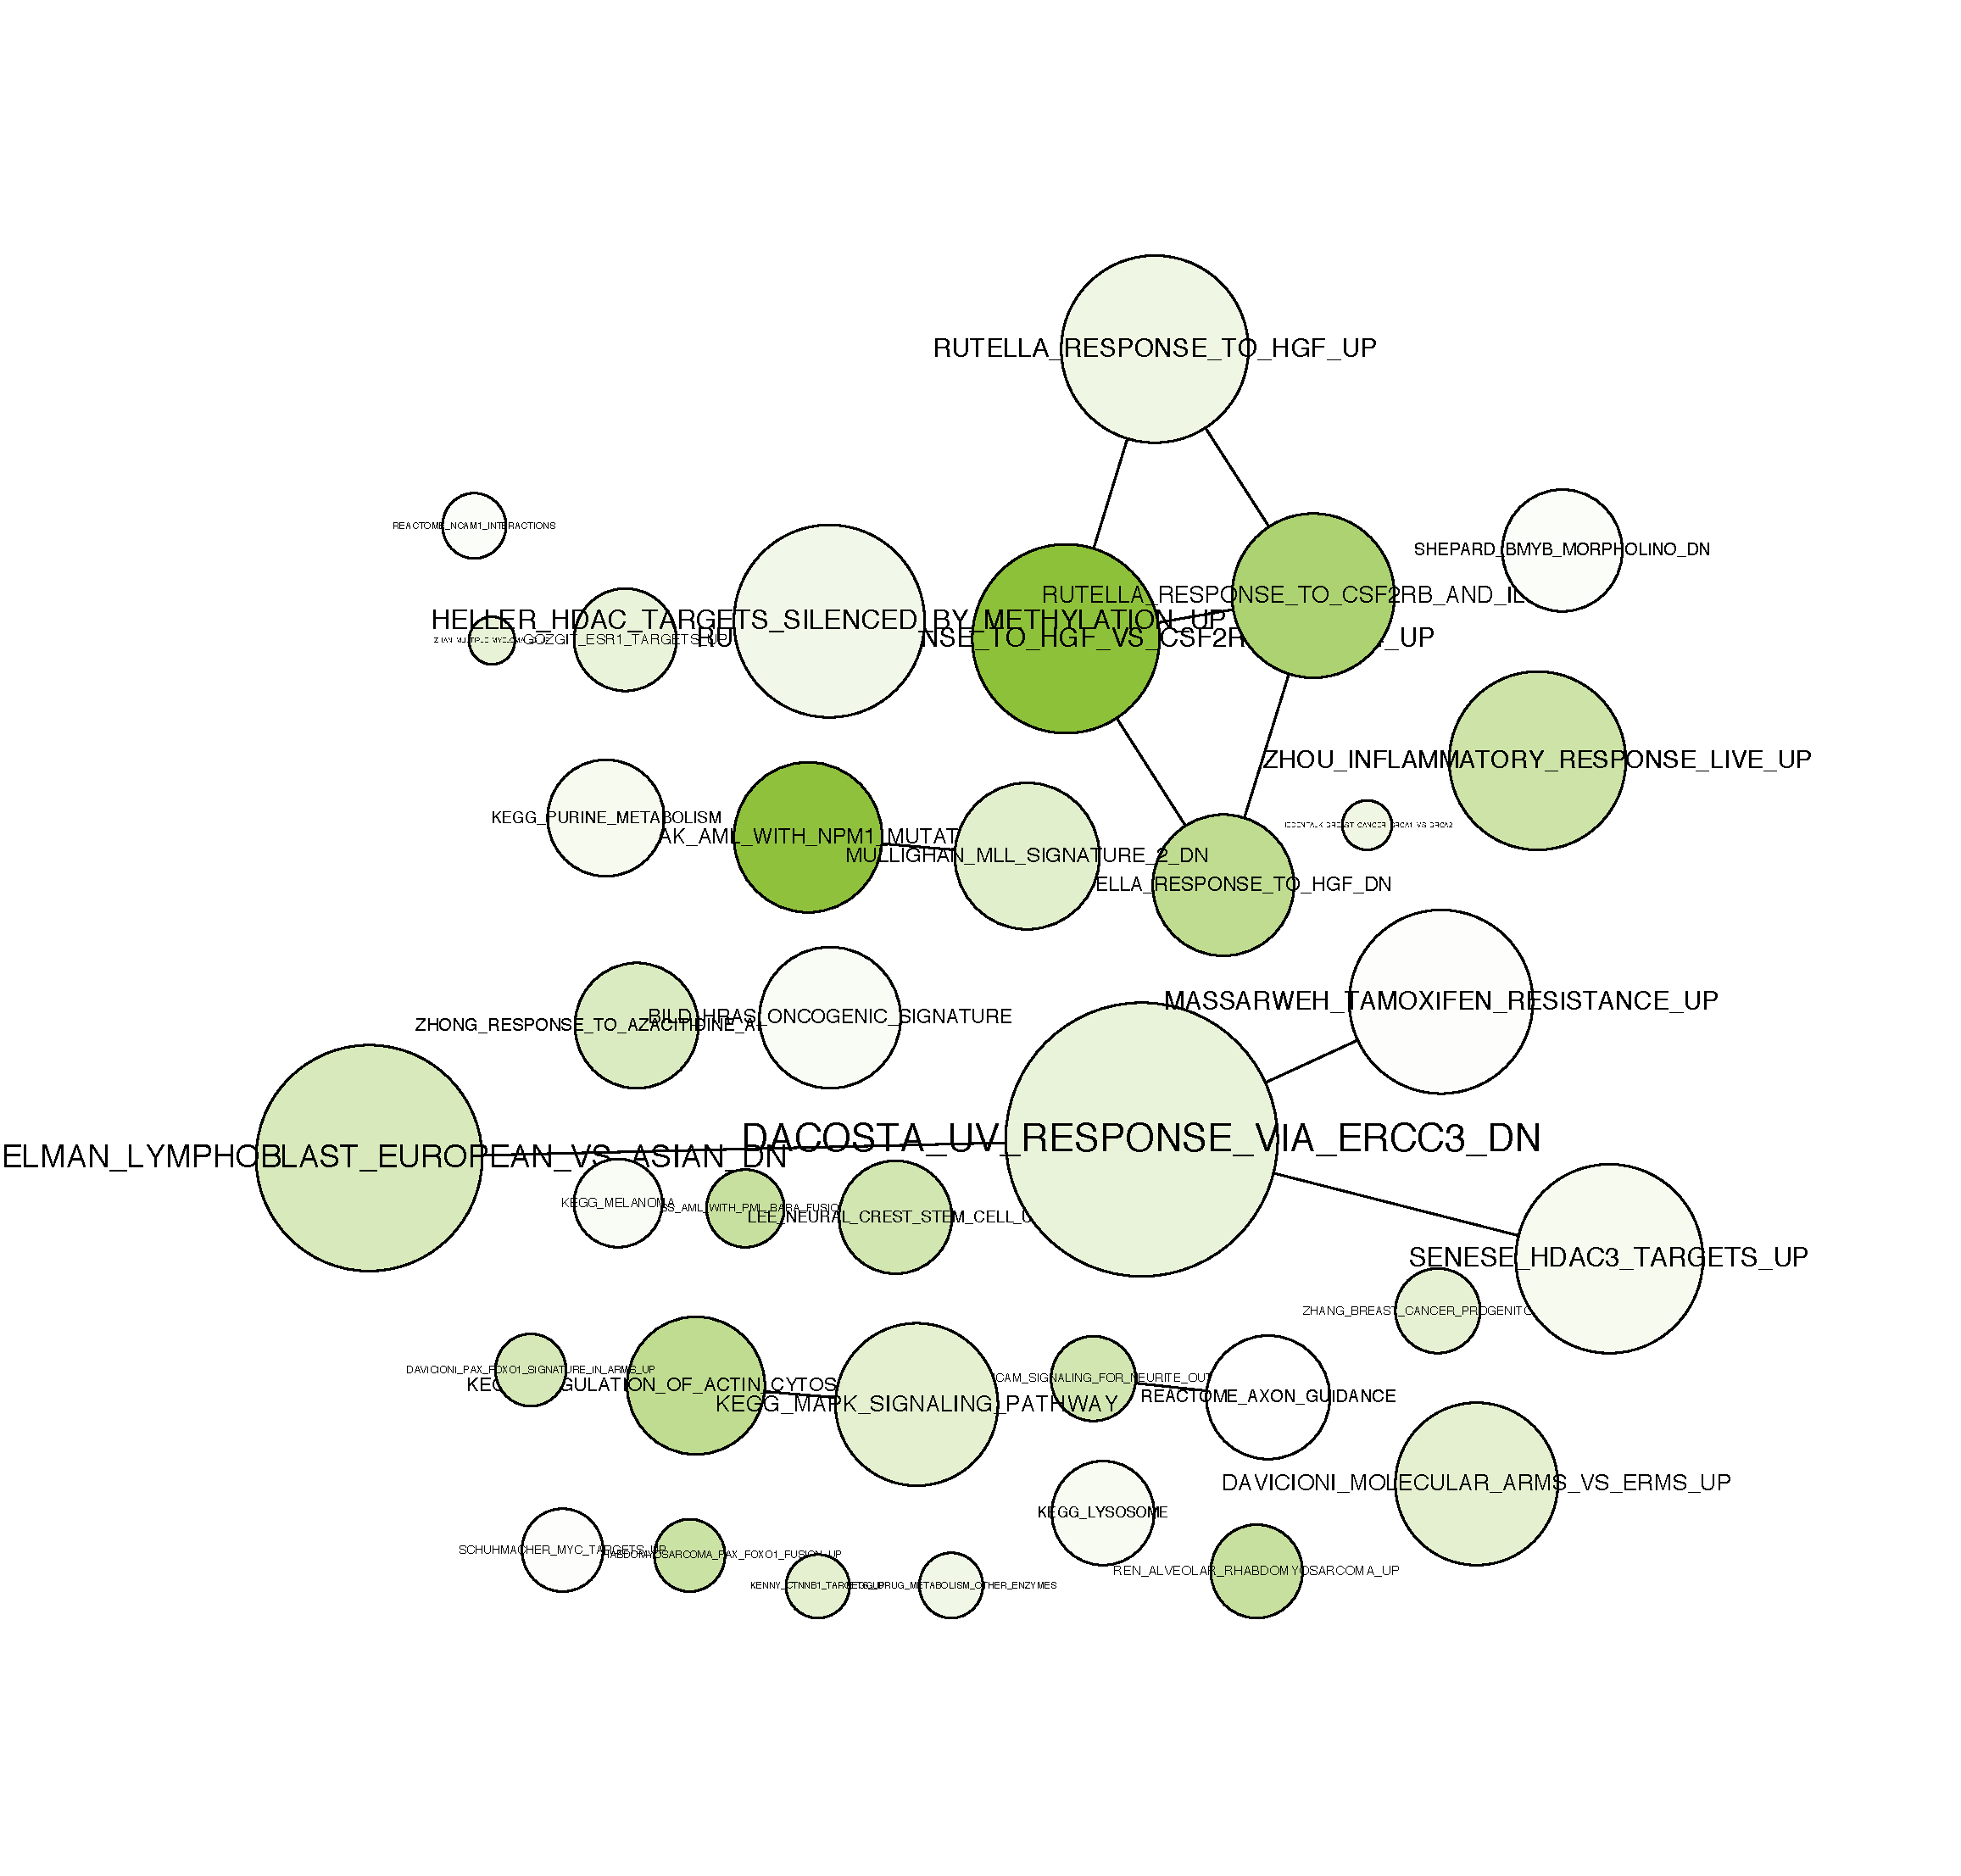
\includegraphics[width=\textwidth]{h838_basal_gage_msigdb.pdf}
\end{center}
\caption[Basal gene set enrichment]{
{\bf Basal gene set enrichment between heterogeneous and homogeneous cocultures.} 
The fold changes between heterogeneous and homogeneous coculture expressions 
for a certain gene set at 0h are compared with the background using $t$ test.
The signicance level (negative log-transformed $p$-value) is color-coded, such
that green means enrichment of a gene set and white means depletion. The size
of the gene set is coded by the size of the circles.
}
\label{fig:h838_basal_gage_msigdb}
\end{figure}

\begin{figure}[!ht]
\begin{center}
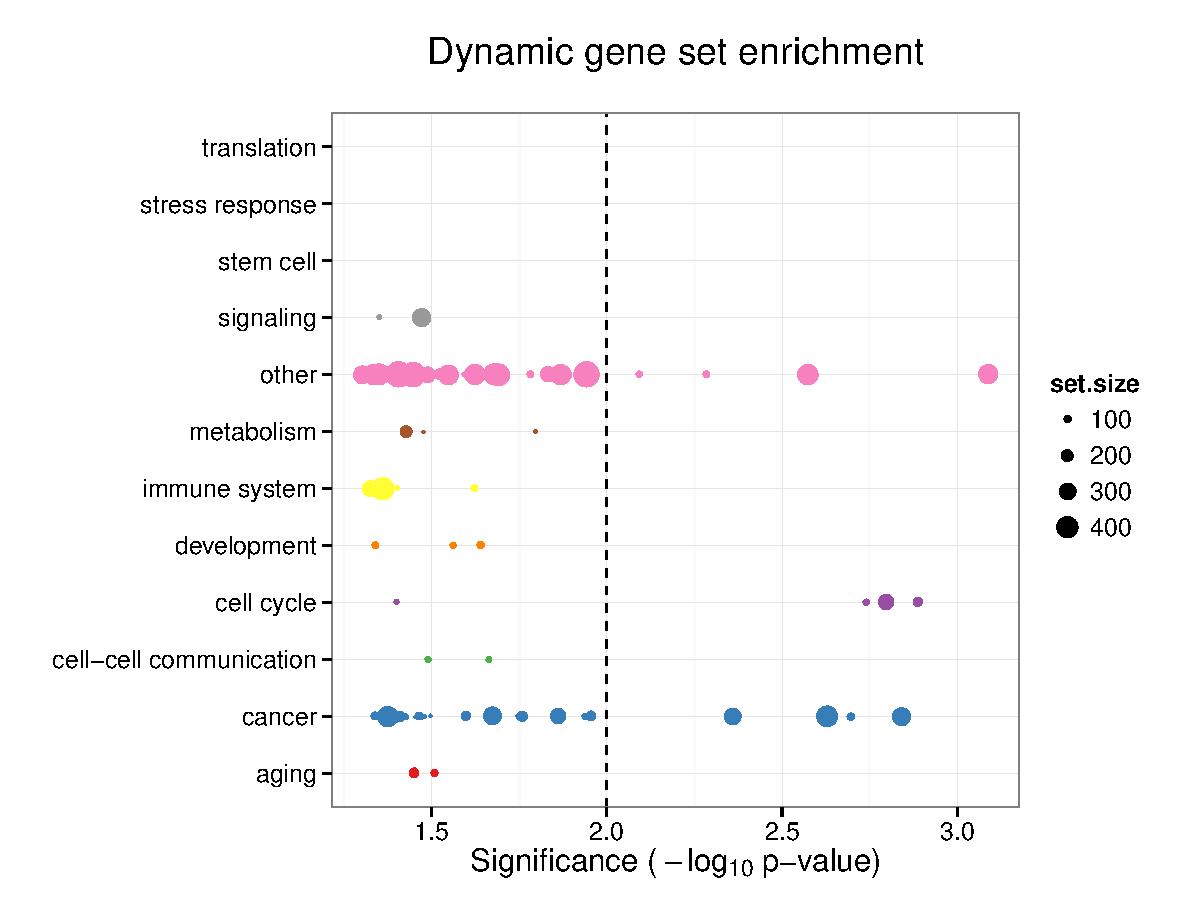
\includegraphics[width=\textwidth]{h838_dynamic_gage_msigdb.pdf}
\end{center}
\caption[Dynamic gene set enrichment]{
{\bf Dynamic gene set enrichment between heterogeneous and homogeneous 
cocultures.} 
The differential expression of each gene is first assessed by the full/reduced
model (\ref{sec:full_reduced}), the mean differential score of a gene set
is then compared with that of the background set using $t$ test.
The signicance level (negative log-transformed $p$-value) is color-coded, such
that green means enrichment of a gene set and white means depletion. The size
of the gene set is coded by the size of the circles.
}
\label{fig:h838_dynamic_gage_msigdb}
\end{figure}

The functional association of the transcriptome response, however, can be
decoded in a fine-tuned gene set enrichment test between the 0h unscratched
sample and each of the other time points. In the heteregeneous coculture 
(\ref{fig:h838_hetero_gage}),
we see an initial enrichment of gene sets related to breast cancer, terms
such as metastasis are over-represented between 1 and 2 hours, which are
again followed by cell migration related gene sets at 4h. After 5 hours,
the functions of enriched gene sets diverge and become less specific.
In contrast, although the enriched gene sets of homogeneous coculture also 
include cancer-related terms, there is no visible general trend that can
be followed over time (\ref{fig:h838_homo_gage}). 

\begin{figure}[!ht]
\begin{center}
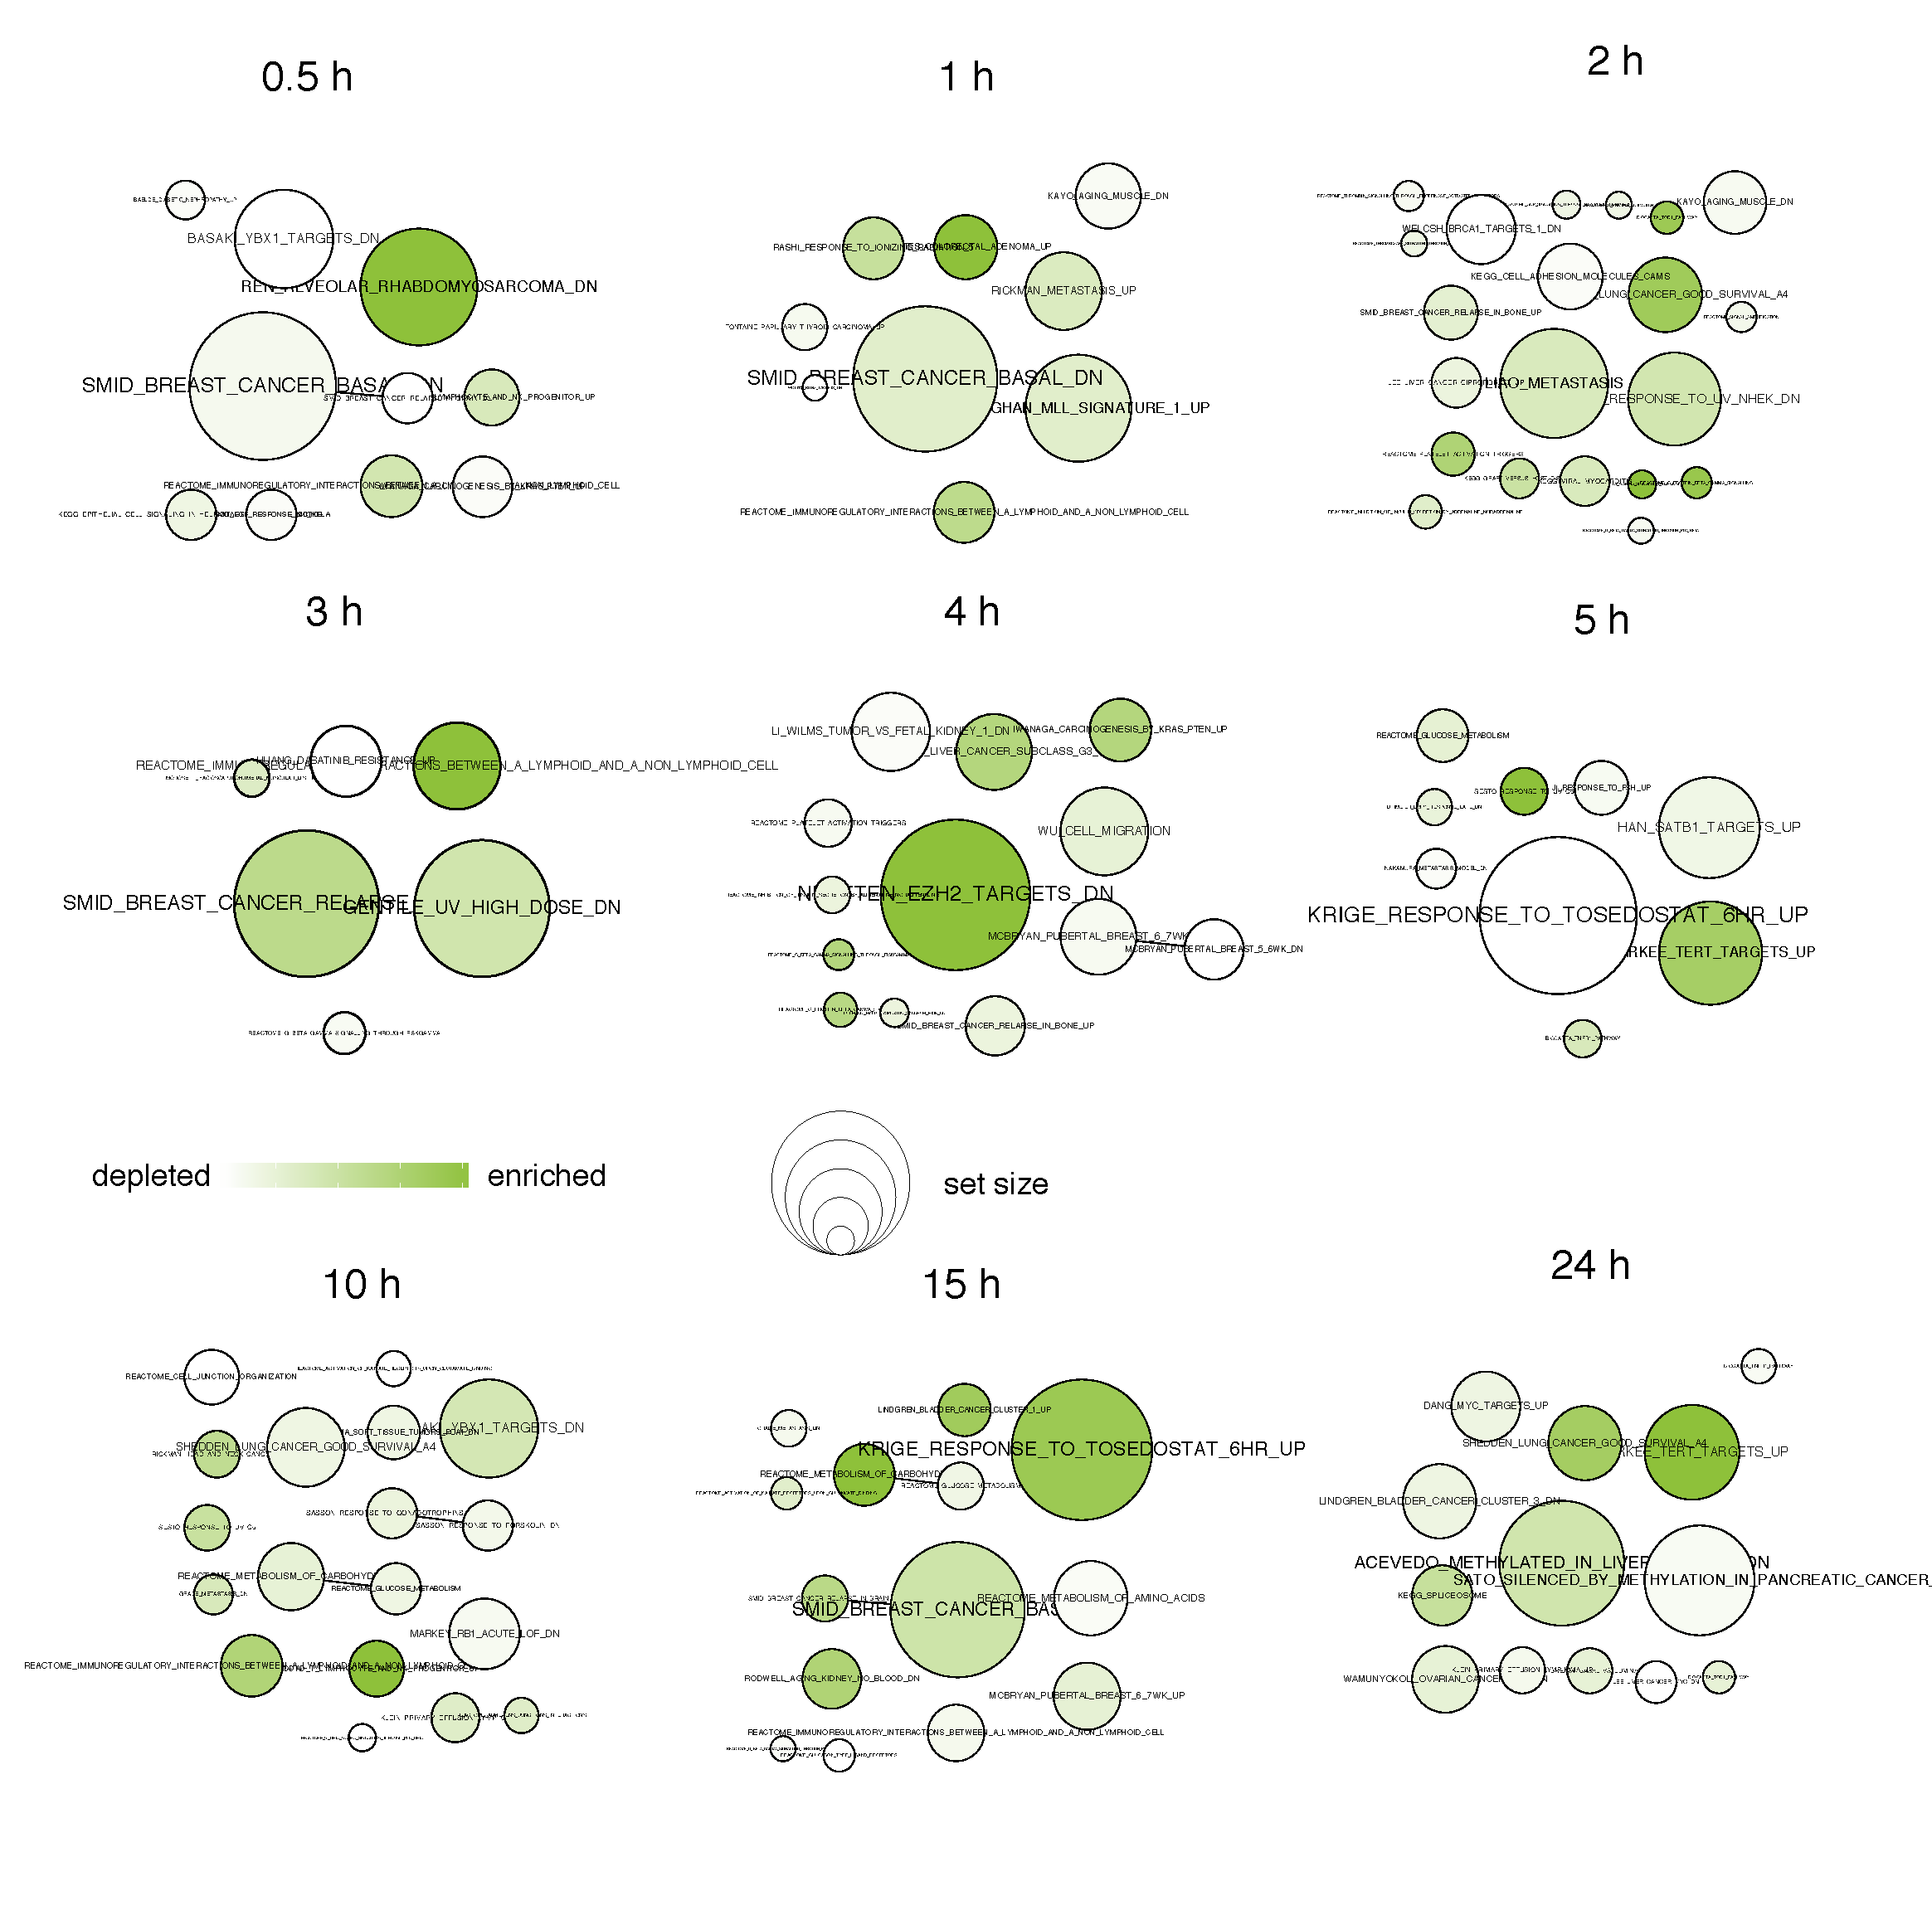
\includegraphics[width=\textwidth]{h838_HMEC_gage.pdf}
\end{center}
\caption[Dynamic gene set enrichment]{
{\bf Dynamic gene set enrichment between heterogeneous and homogeneous 
cocultures.} 
The differential expression of each gene is first assessed by the full/reduced
model (\ref{sec:full_reduced}), the mean differential score of a gene set
is then compared with that of the background set using $t$ test.
The signicance level (negative log-transformed $p$-value) is color-coded, such
that green means enrichment of a gene set and white means depletion. The size
of the gene set is coded by the size of the circles.
}
\label{fig:h838_hetero_gage}
\end{figure}

\begin{figure}[!ht]
\begin{center}
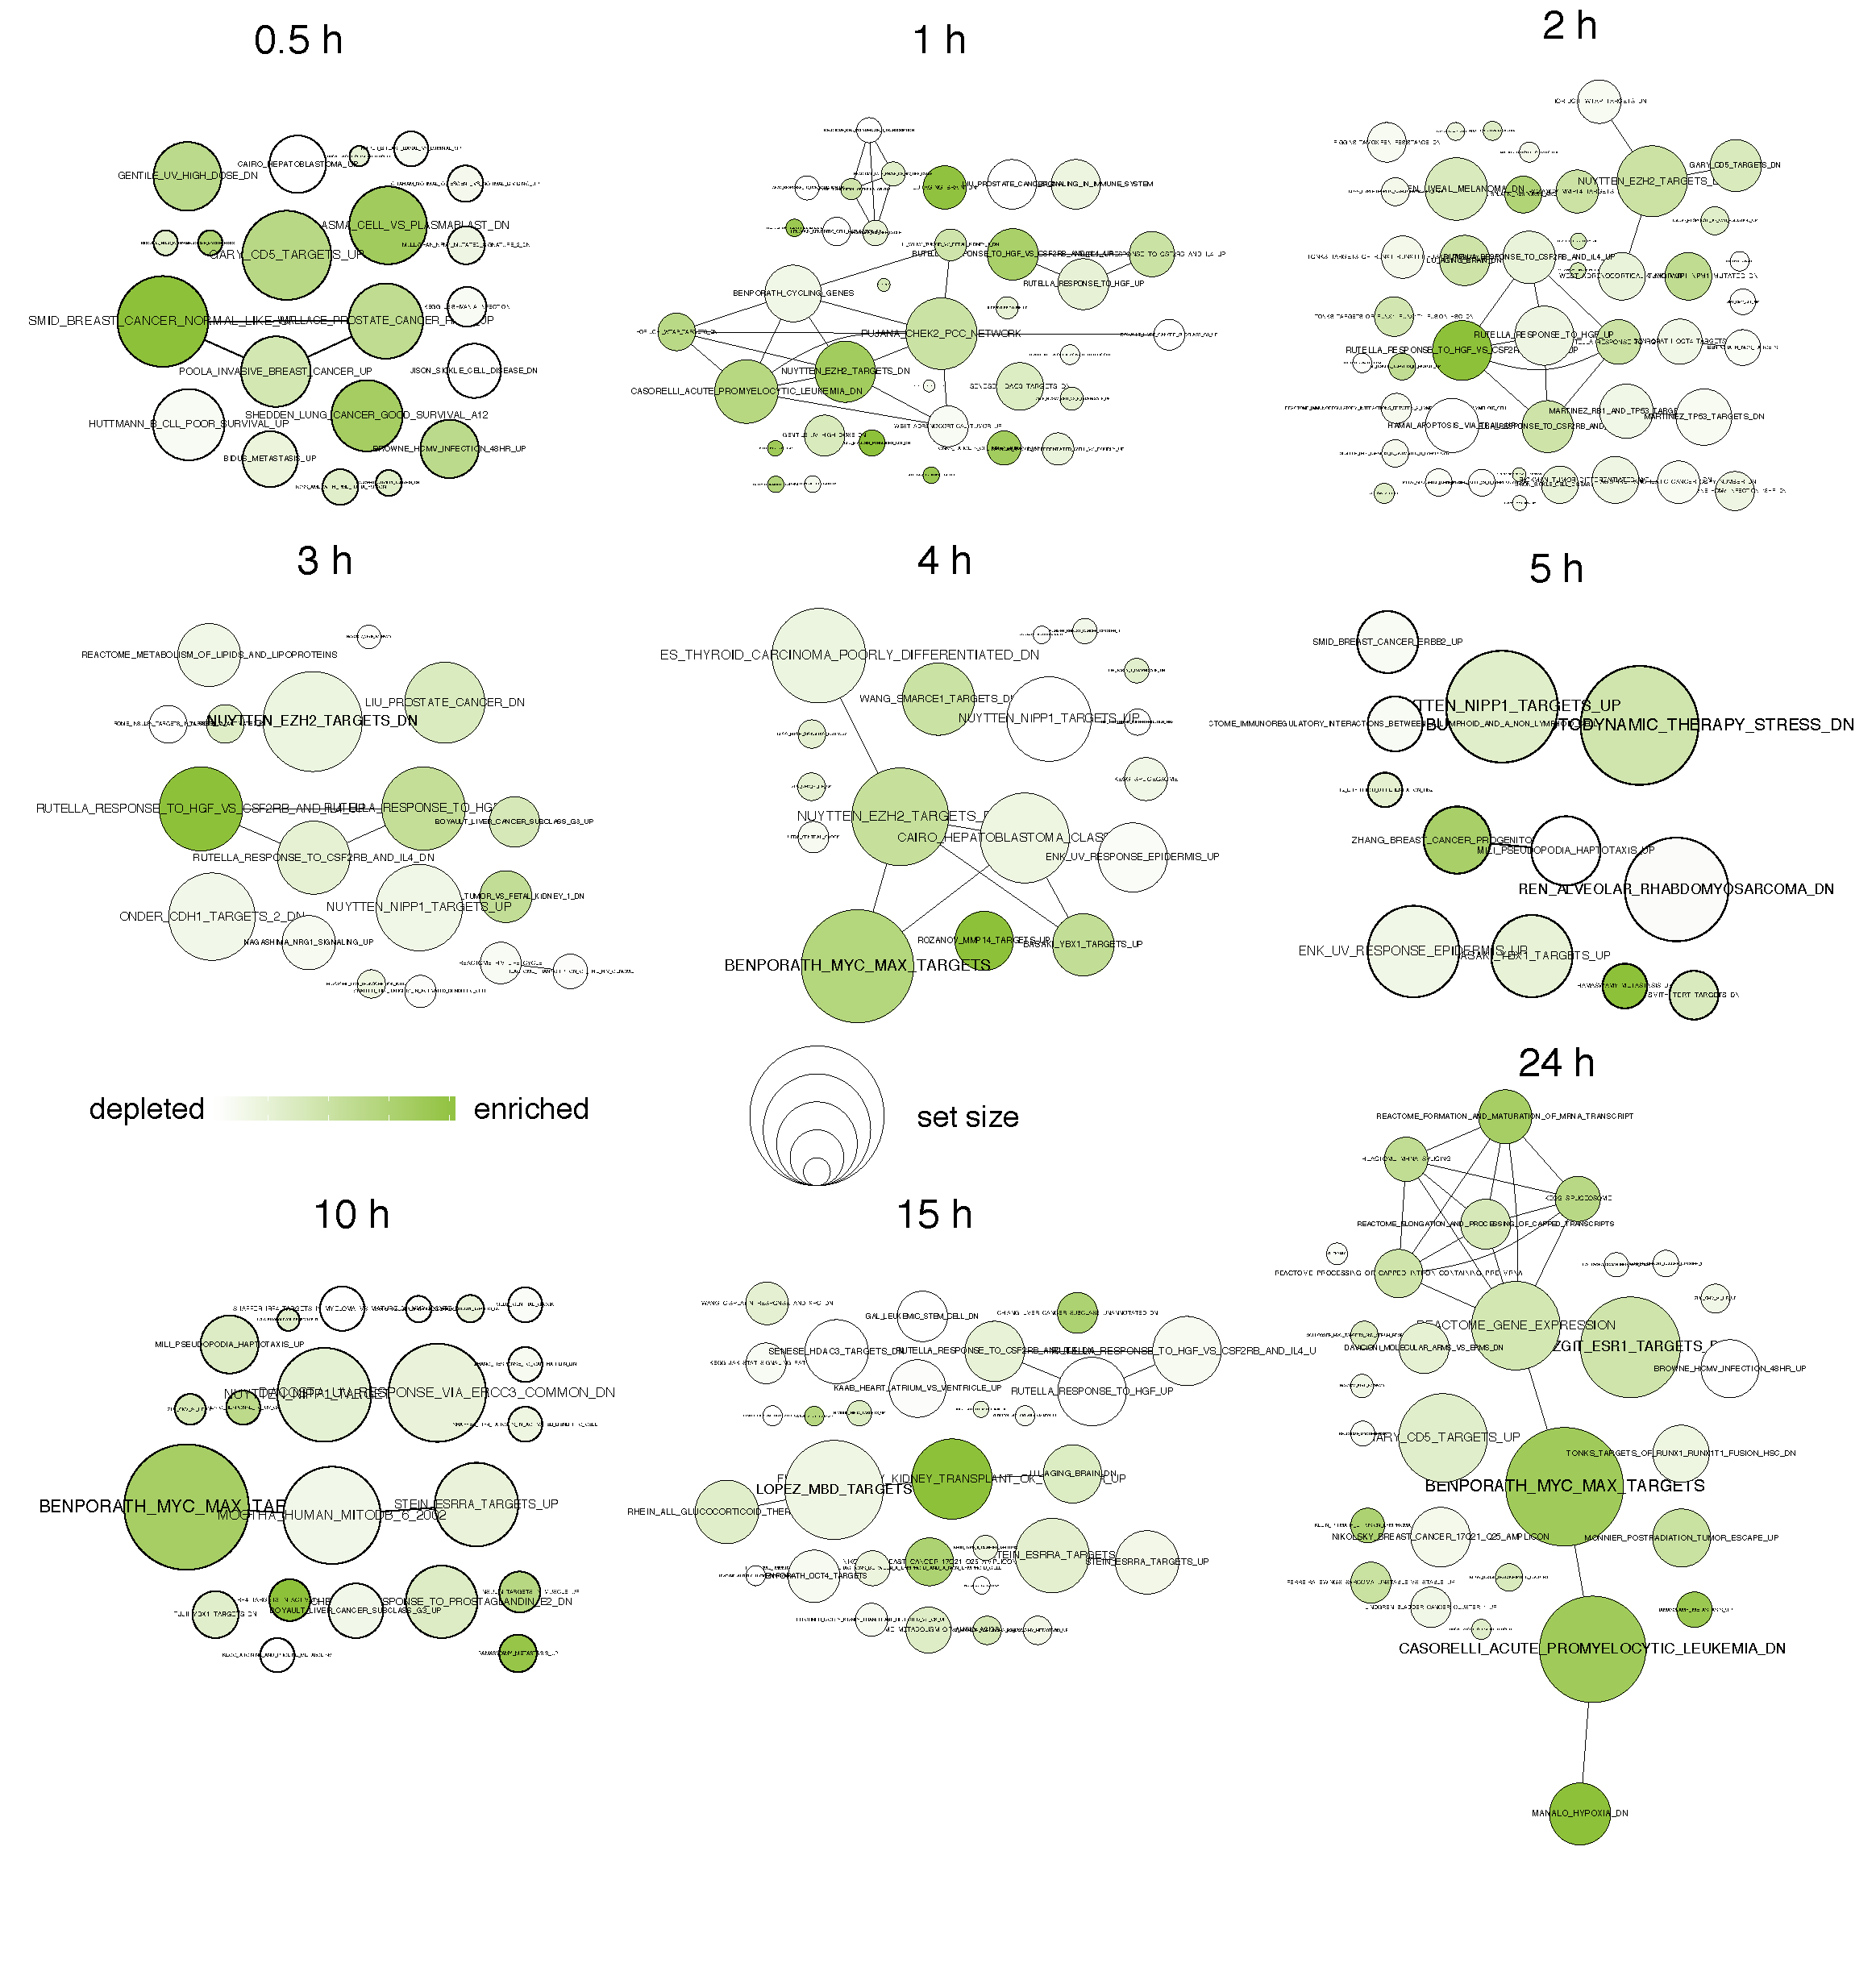
\includegraphics[width=\textwidth]{h838_Mono_gage.pdf}
\end{center}
\caption[Dynamic gene set enrichment]{
{\bf Dynamic gene set enrichment between heterogeneous and homogeneous 
cocultures.} 
The differential expression of each gene is first assessed by the full/reduced
model (\ref{sec:full_reduced}), the mean differential score of a gene set
is then compared with that of the background set using $t$ test.
The signicance level (negative log-transformed $p$-value) is color-coded, such
that green means enrichment of a gene set and white means depletion. The size
of the gene set is coded by the size of the circles.
}
\label{fig:h838_homo_gage}
\end{figure}

We further investigated
the enrichment of KEGG pathways for both heterogeneous and homogeneous 
coculture (\ref{fig:h838_gage_kegg}). By grouping the time points into 3 
consecutive phases (early,
intermediate, late), we can identify the MAPK signaling pathway as a prominent 
candidate in the heteregeneous coculture. The MAPK pathway also shares 
member proteins with other pathways, as indicated by the edges in 
\ref{fig:h838_gage_kegg}, which hints at the possibility of the MAPK pathway
crosslinking with other signaling pathways.\footnote{We also discuss this
result later in detail.} On the other hand, a number of different pathways 
are over-represented in the homogeneous coculture, whereas the MAPK
pathway is absent.

\begin{figure}[!ht]
\begin{center}
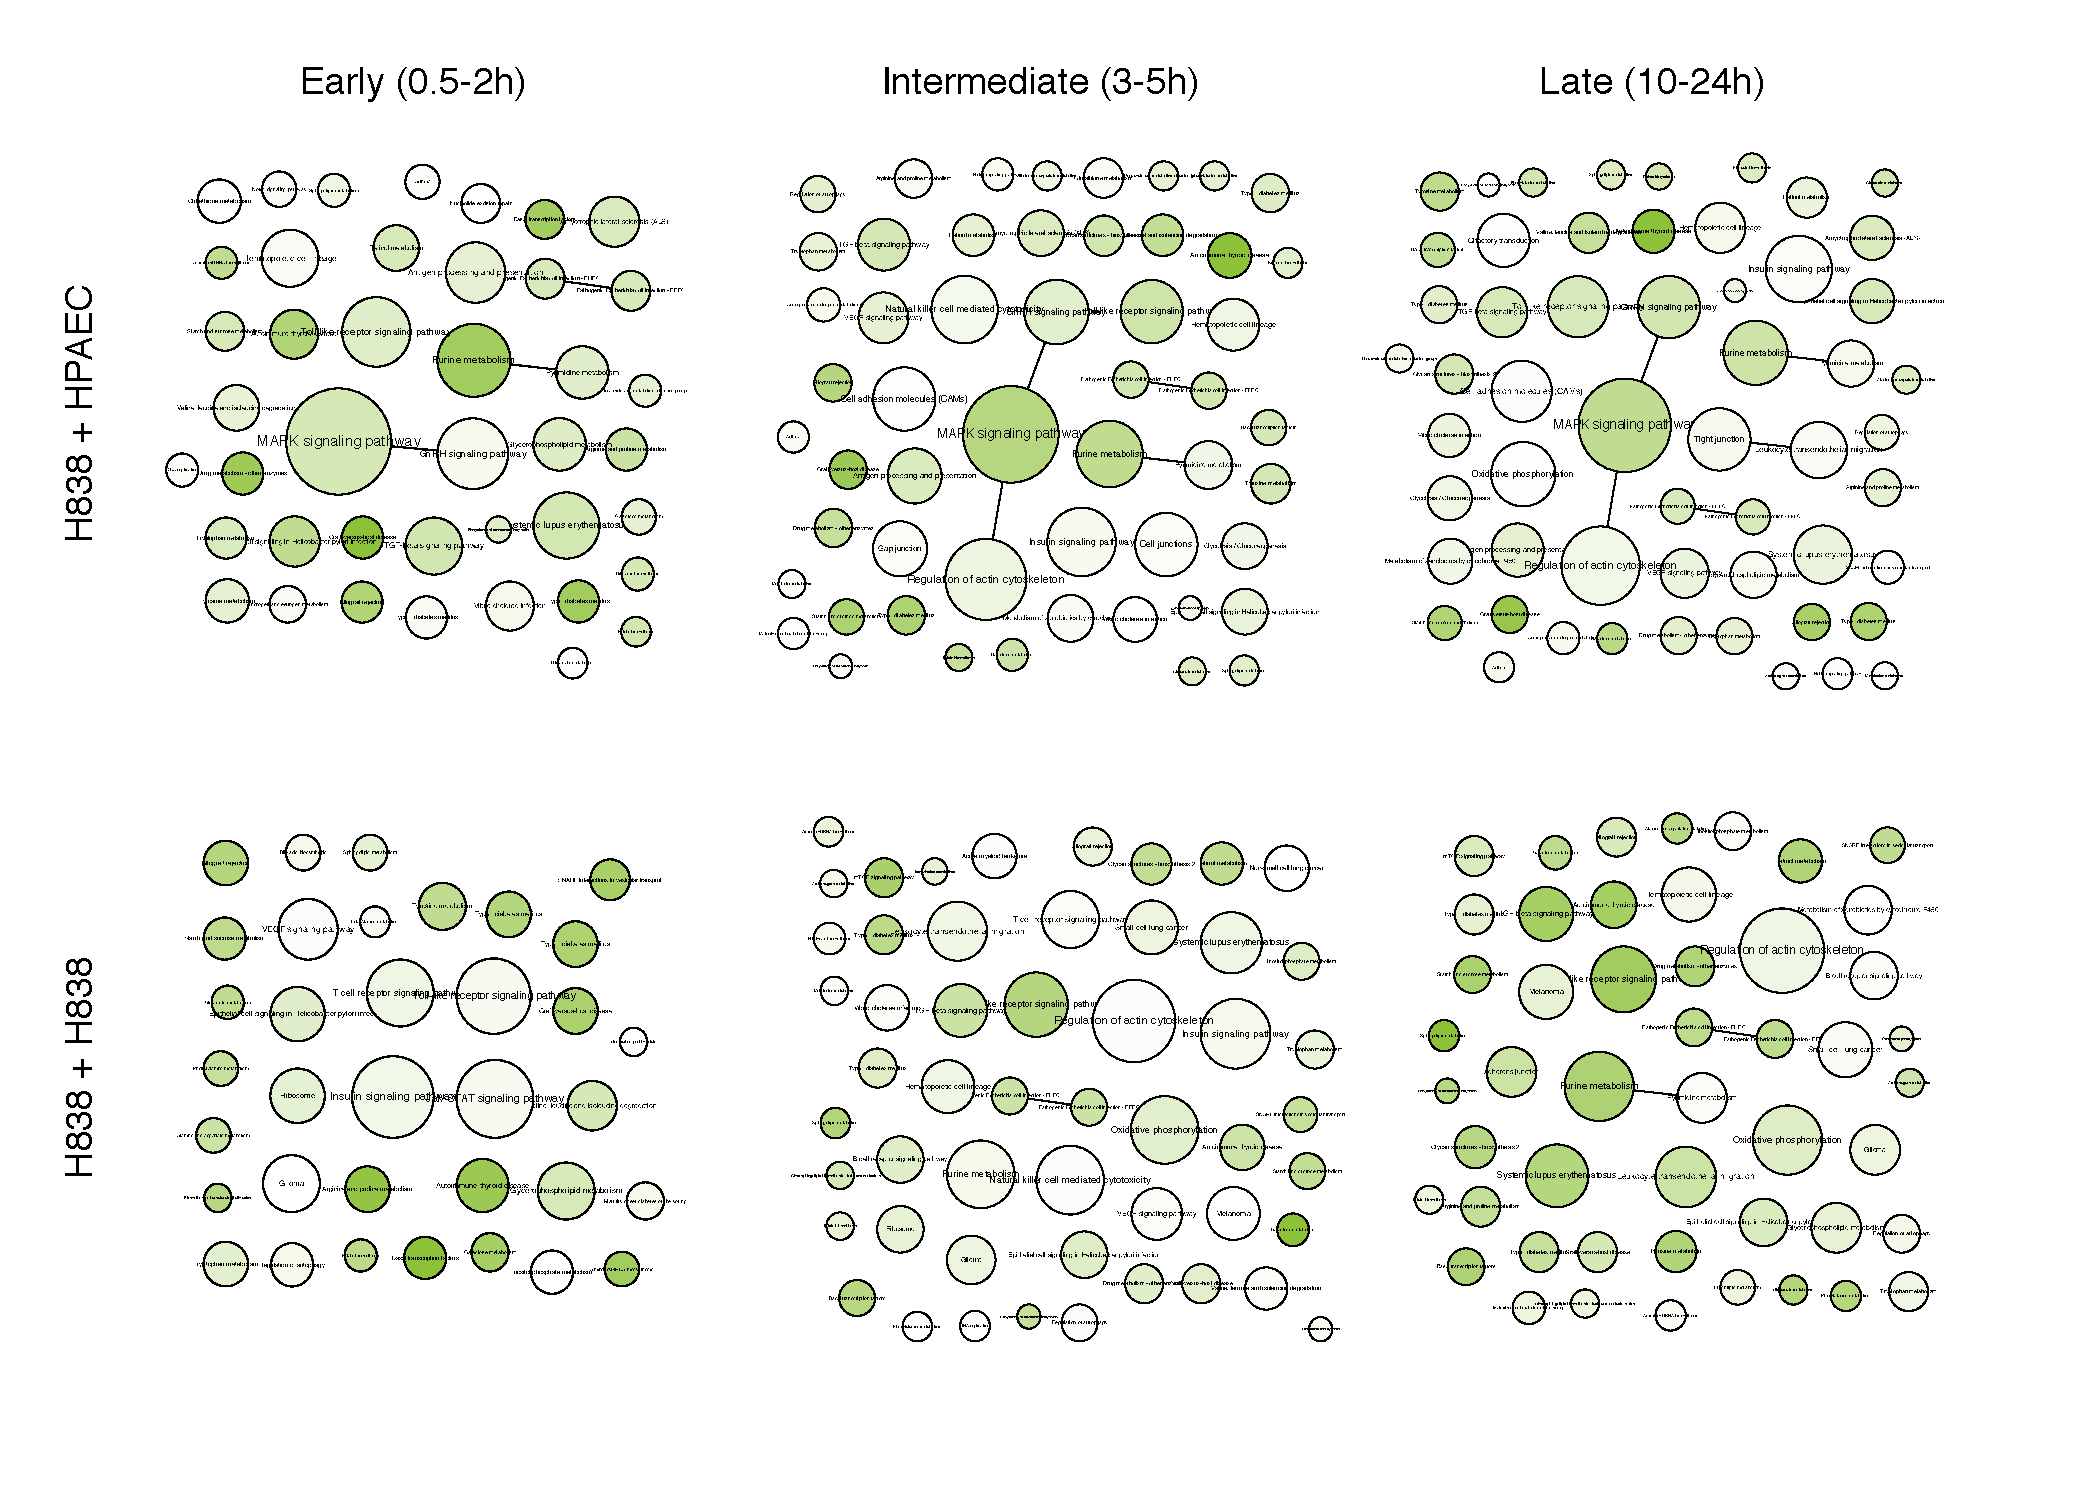
\includegraphics[width=\textwidth]{h838_gage_kegg.pdf}
\end{center}
\caption[Dynamic gene set enrichment]{
{\bf Dynamic gene set enrichment between heterogeneous and homogeneous 
cocultures.} 
The differential expression of each gene is first assessed by the full/reduced
model (\ref{sec:full_reduced}), the mean differential score of a gene set
is then compared with that of the background set using $t$ test.
The signicance level (negative log-transformed $p$-value) is color-coded, such
that green means enrichment of a gene set and white means depletion. The size
of the gene set is coded by the size of the circles.
}
\label{fig:h838_gage_kegg}
\end{figure}

\subsubsection{Identification of putative transcription factors in the H838 gene regulation}

The cellular signal flow, in the form of pathway activation
downstream from membrane receptors and the subsequent 
transcriptional 
regulation, is made non-trivial by the fact that proteome 
and transcriptome regulation changes have different time scales~\citep{Busch2008}. 
To overcome this difficulty, we infer the signal flow by 
tracing the cause of the transcriptome dynamics back to the external stimuli via putative transcription factors, protein-protein interaction
and receptor activation. 

We first applied a gene set enrichment test for the gene expression at 
the different time points using the transcription factor target gene sets (The Molecular Signature Database).
For each time point, 
genes were ranked according to their fold expression values
between the homo- and heterogenous coculture responses. 
A $t$-test is subsequently performed for each
transcription factor target gene set at a certain time 
point compared to the 
background set.

All significantly ($p$-value $<0.05$) enriched 
transcription factors at individual time points are 
depicted in \ref{fig:h838_tf}. Up to 2 hours, nuclear
factor family, AP-1 complex (JUN, FOS) and other diverse
transcription factors are active and responsible for 
inducing immediate early genes. Between 3 and 4 hours after
scratch, several E2F and E4F transcription factors take
over the control and effectively become the secondary 
transcriptional regulators. Active transcription factors
at later time points are less in number than the early 
active ones.
Taken together, applying the gene set
enrichment method on the time-resolved microarray data, we identified here the
sequence of putatively enriched transcription factor targets, which could also serve as
a proxy for the temporal activity of transcription factors \emph{per se}.

\begin{figure}[!ht]
%\newpage
\begin{center}
%\captionsetup{labelformat=prepage}
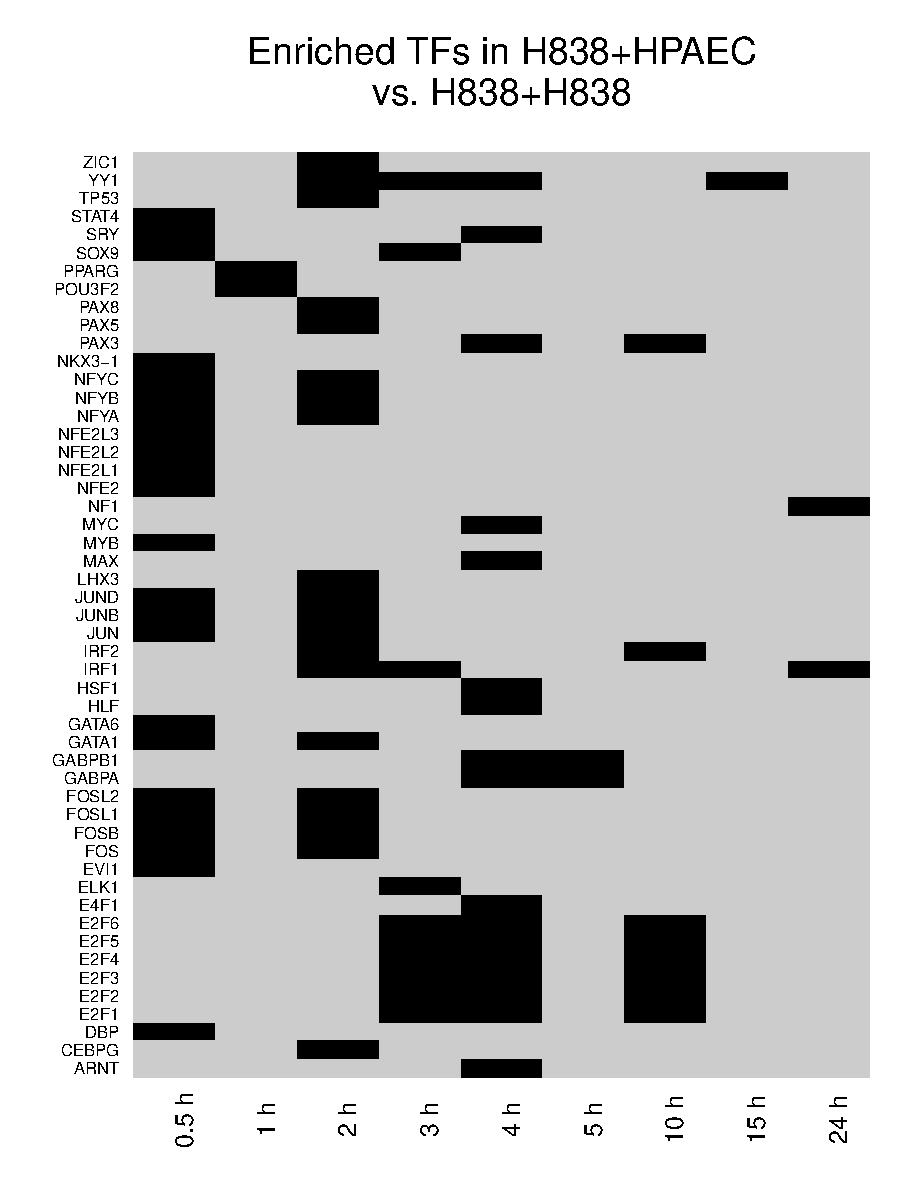
\includegraphics[width=0.8\textwidth]{h838-tf_heatmap.pdf}
\end{center}
\caption[Enrichment of transcription factors]{
{\bf Enrichment of transcription factor target genes in
the H838 cells cocultured with HPAEC at each time point.} 
Black squares indicate the over-representation ($p<0.05$) of the  
target genes regulated by a particular transcription factor
at a given time point, while gray squares indicate the
absence of such enrichment.
}
\label{fig:h838_tf}
\end{figure}

\subsubsection{Data-mining the pathways from cytokine receptors to transcription factors and gene response}

To further bridge the gap between the transcription factors identified above and the membrane cytokine receptors that 
transmit the external signal,
we mapped shortest paths from each cytokine receptor to all putative transcription factors, using both a directed~%
\citep{Vinayagam2011} and undirected~\citep{Schaefer2012} 
protein-protein interaction network.  

As depicted in \ref{fig:h838_receptor_ts_ex}, the inverse
mean first passage time (MFPT) and inverse shortest path 
(SP) show totally different dynamics. We further use the
area under the curve (AUC) of inverse distances as a 
measure of proximity and thus functional relatedness between
receptors and transcription factors (TF). 
The larger the AUC is,
the more likely, we hypothesize, that the signal is
transmitted through this receptor downward to the 
corresponding TFs. We also calculate the probability of
obtaining a certain AUC by chance, which is the fraction
of AUC between the receptor and bootstrapped TFs that are
more extreme than the actual AUC 
(\ref{fig:h838_receptor_pval_ex}).

\begin{figure}[!ht]
\begin{center}
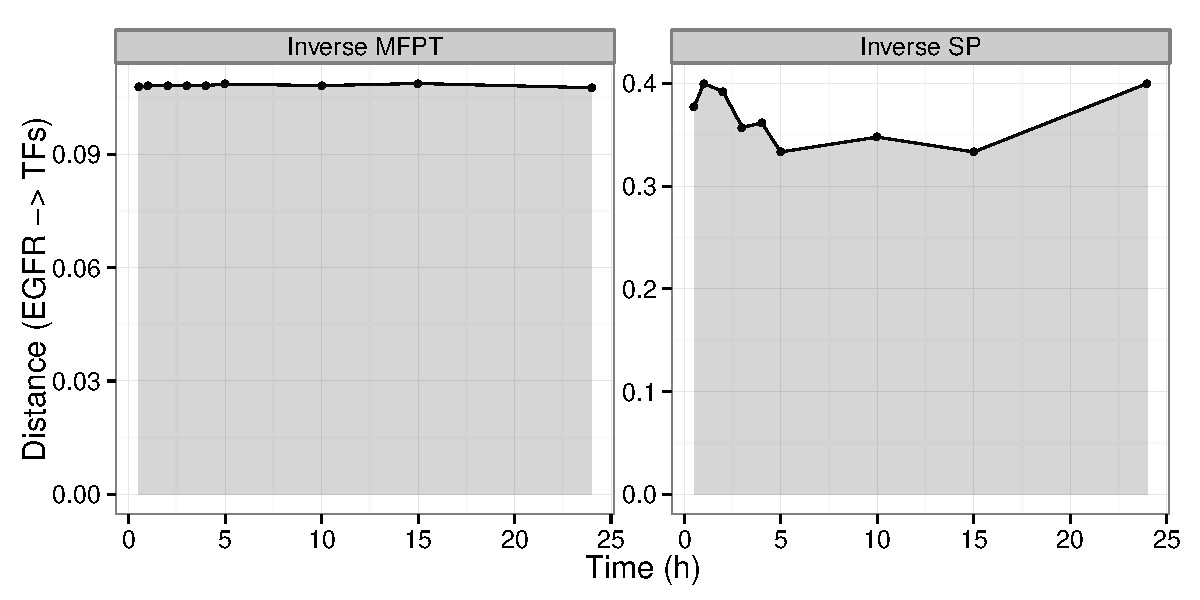
\includegraphics[width=\textwidth]{h838-receptor_ts_ex_hppi.pdf}
\end{center}
\caption[Inverse distance over time]{
{\bf Inverse nodal distance from EGFR to enriched 
transcription factors at each time point.} 
Inverse distance is measured by mean first passage time
(MFPT) and shortest path (SP) respectively. Shaded area
indicates the area under the curve (AUC) used to 
characterize the overall proximity between a given
receptor and all enriched transcription factors.
}
\label{fig:h838_receptor_ts_ex}
\end{figure}

\begin{figure}[!ht]
\begin{center}
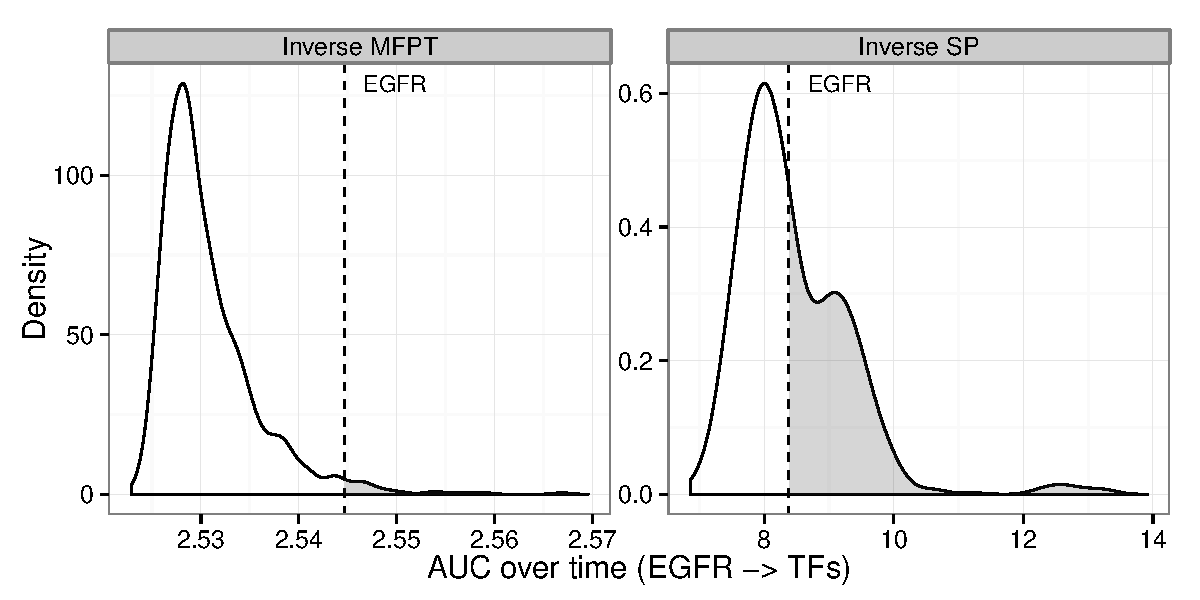
\includegraphics[width=\textwidth]{h838-receptor_pval_ex_hppi.pdf}
\end{center}
\caption[Significance of the inverse distance AUC]{
{\bf Significance of the inverse distance AUC from EGFR to
all enriched transcription factors.} 
Shown is the distribution of the inverse distance AUC from
EGFR to all enriched transcription factors (TF). 
The distribution
is determined by calculating the inverse distance between
EGFR and randomly selected TFs.
AUC is calculated for inverse MFPT and SP as in 
\ref{fig:h838_receptor_ts_ex}. Dashed vertical line
denotes the AUC from EGFR to the TFs identified from the
data, shaded area is the region that the bootstrapped 
AUC is more extreme than the actual value and is thus used
to calculate the $p$-value.
}
\label{fig:h838_receptor_pval_ex}
\end{figure}

In summary, if we rank the receptors by their inverse
shortest path AUC (\ref{fig:h838_receptor_auc_sp}), we
can easily identify certain candidate receptors that
are likely responsible for the signal flow from the external
stimulus to the downstream transcription factors. 
Interleukin and TNF receptors are two big families of 
membrane receptors. Most of the interleukin receptors have
a significant AUC as measured by the inverse shortest path,
whereas none of the TNF receptor super family members has
a $p$-value less than 0.05. Therefore, neither of both 
classes provides a highly discriminative candidate receptor.
Among the chemokine (C-X-C motif) receptors, CXCR4 stands
out. In terms of the chemokine (C-C motif) receptors, 
CCR5/1/2 are the hits that are most likely related to the
signal flow. Yet other receptors can be identified that
have both a high AUC and a significant $p$-value.
In contrast, all receptors show a homogeneous distribution
of both AUC and $p$-value when ranked according to the 
inverse mean first passage time 
(\ref{fig:h838_receptor_auc_mfpt}), which is thus of
limited use in this specific case.

\begin{figure}[!ht]
\begin{center}
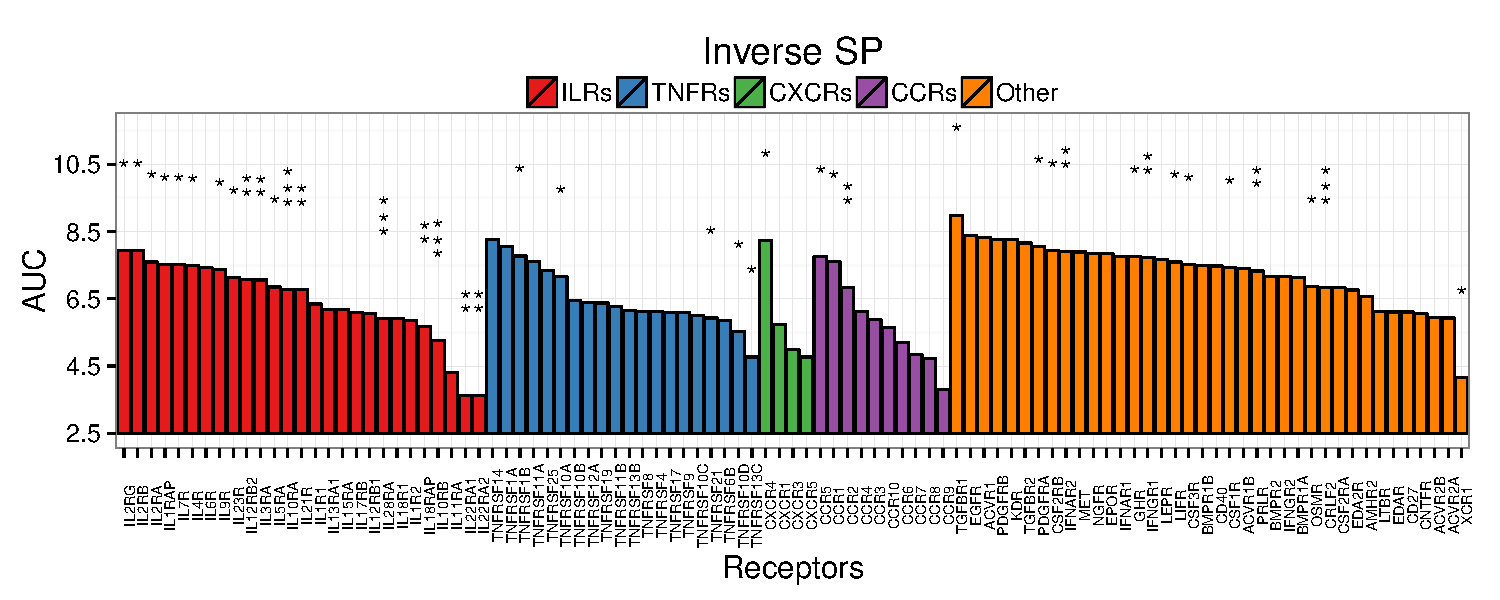
\includegraphics[width=\textwidth]{h838-receptor_auc_sp_hppi.pdf}
\end{center}
\caption[Receptor ranking by inverse SP]{
{\bf Receptor ranking by the AUC of inverse shortest path.} 
Receptors are grouped into 5 major categories and ranked
according to their AUC of shortest path to all enriched TFs.
Asterisks indicate the $p$-value of the AUC as determined by
bootstrapping. ***: $p<0.01$, **: $p<0.05$, *: $p<0.1$.
}
\label{fig:h838_receptor_auc_sp}
\end{figure}

\begin{figure}[!ht]
\begin{center}
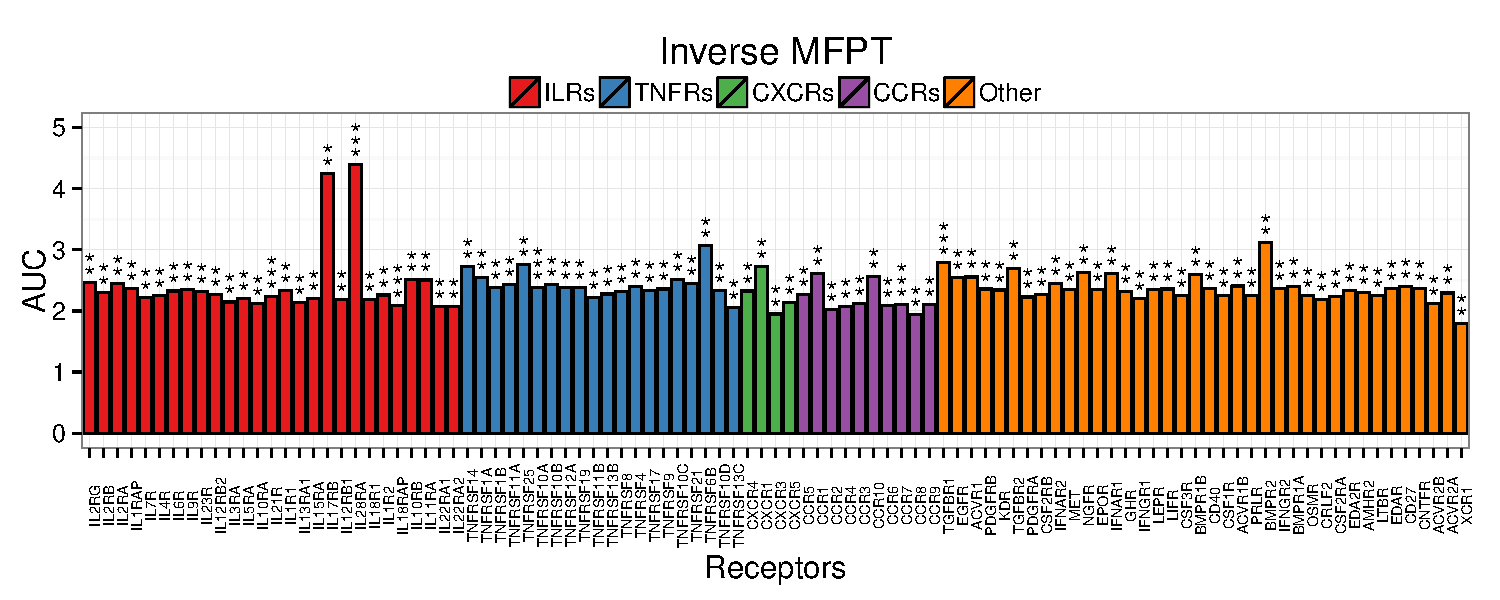
\includegraphics[width=\textwidth]{h838-receptor_auc_mfpt_hppi.pdf}
\end{center}
\caption[Receptor ranking by inverse MFPT]{
{\bf Receptor ranking by the AUC of inverse mean first 
passage time.} 
Receptors are grouped into 5 major categories and ranked
according to their AUC of MFPT to all enriched TFs.
Asterisks indicate the $p$-value of the AUC as determined by
bootstrapping. ***: $p<0.01$, **: $p<0.05$, *: $p<0.1$.
}
\label{fig:h838_receptor_auc_mfpt}
\end{figure}

\begin{figure}[!ht]
\begin{center}
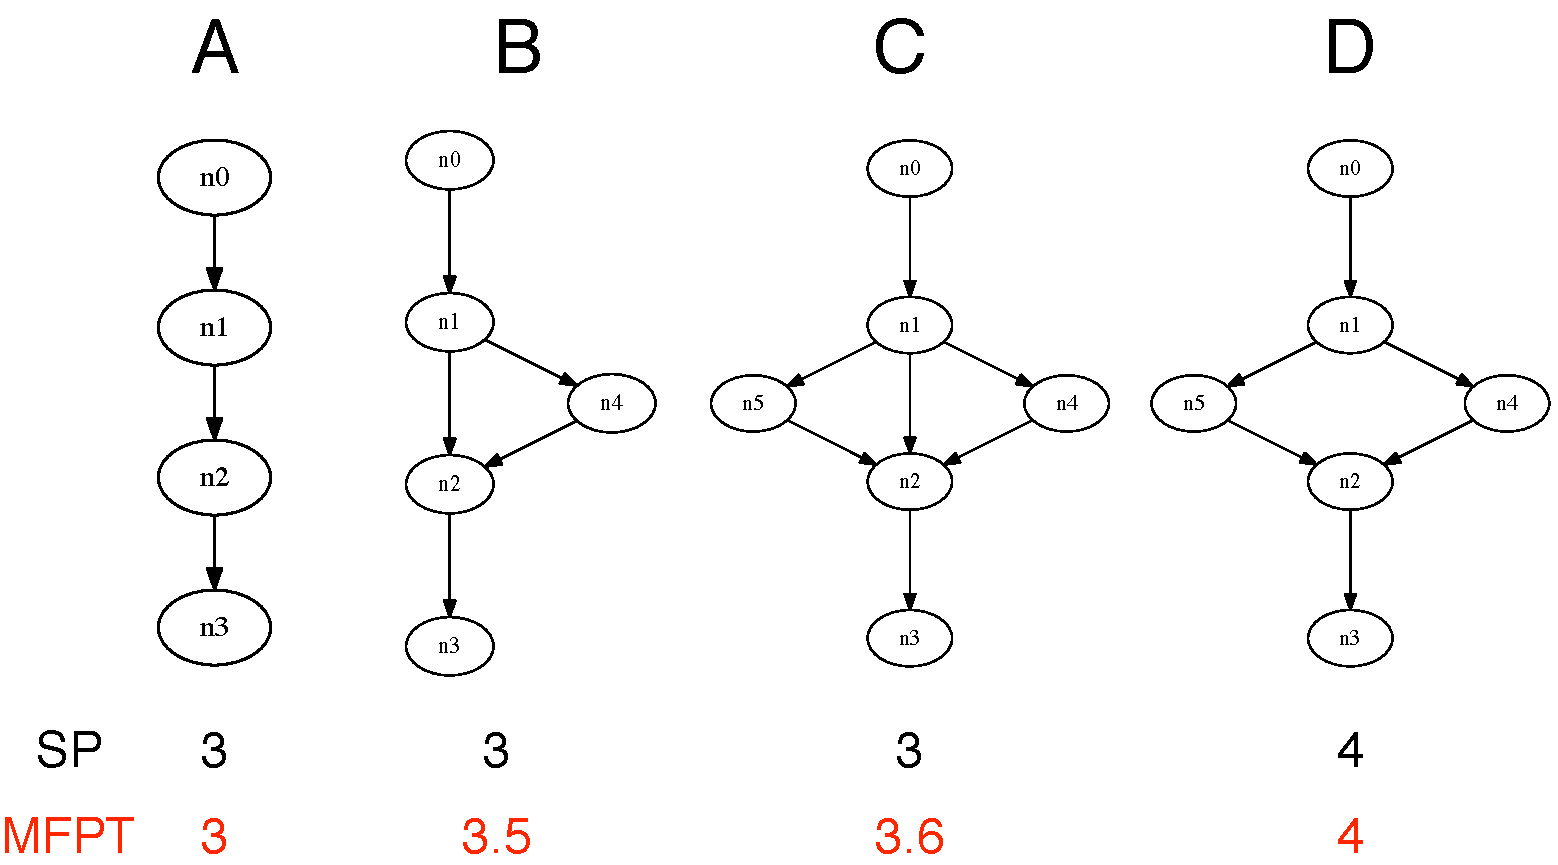
\includegraphics[width=\textwidth]{mfpt_directed_toy.pdf}
\end{center}
\caption[Toy example of SP and MFPT on different directed networks]{
{\bf Comparison of shortest path (SP) length and mean first passage time 
(MFPT) on different directed toy networks.}
Shown are the distances between node $n0$ and $n3$ measured in shortest path 
(SP) and mean first passage time (MFPT) respectively.
}
\label{fig:mfpt_directed_toy}
\end{figure}

\subsubsection{Supernatant  from different co-cultures show distinct cytokine composition}

If the receptors predicted in the previous section are indeed of functional
relevance in the signal processing of tumor cells, we would also expect an
enrichment of the corresponding ligands in the medium,
which mediate the communication between
HPAEC and H838 cells and enhance the tumor cell migration.
To this end, we quantified the cytokine composition
of the  homo- and heterogeneous cocultures
both before and 24h after onset of migration.
We used a  fluorescent bead array based cytokine assay which detects fifty cytokines (\ref{table:cytokine}).

\begin{longtable}{ccccc}
\caption{List of cytokines in the array.} \\ 
\hline
Eotaxin & IL-5 &   IP-10 &  HGF & MCP-3\\
\rowcolor{Gray} FGF basic &  IL-6 &   MCP-1 &  ICAM-1 & M-CSF\\
G-CSF &  IL-7 &   MIP-1$\alpha$ & IFN$\alpha$2 & MIF\\
\rowcolor{Gray} GM-CSF & IL-8 &   MIP-1$\beta$ &  IL-1$\alpha$ & MIG\\
IFN-$\gamma$ &  IL-9&    PDGF bb&  IL-11-R$\alpha$-lokus chemokine & SCF\\
\rowcolor{Gray} IL-1b &  IL-10 &  RANTES & IL-12 (p40) & SCGF-$\beta$\\
IL-1R$\alpha$ &  IL-12 (p70) &  TNF$\alpha$ &   IL-16 &  SDF-1$\alpha$\\
\rowcolor{Gray} IL-2 &   IL-13 &  VEGF &   IL-18 &  TNF$\beta$\\
IL-3 &   IL-15 &  $\beta$-NGF&  IL-2R-$\alpha$ &   TRAIL\\
\rowcolor{Gray} IL-4 &   IL-17 &  GRO$\alpha$ &  LIF &VCAM-1\\
\hline
\label{table:cytokine}
\end{longtable}
\newpage

A total of twenty-four different cytokines were present in detectable amounts,
fifteen of which showed significant differential upregulation
(\ref{fig:cytokine} A).
% Should add here an additional table with the quantification of all cytokines
Gro-$\alpha$, MCP-3, IL-6, IL-8, IL-13, FGF basic, G-CSF, IP-10 and RANTES were
upregulated in the heterogeneous coculture prior to cell migration.
MIF, IL-12, IL-15, MCP-1 and TNF-$\alpha$ were also upregulated
in the heterogeneous cocultures, and this upregulation was increasing
during tumor cell migration.
Finally, SDF-1$\alpha$ was only found in the heterogeneous coculture,
and was also upregulated after scratching. 

% Need a better headline for the subsection here 
\subsubsection{Isolation of cytokines relevant to migration}

Based on the previous results, 
we found that the upregulated \sdfonea,
RANTES, MCP-1 are the ligands for CXCR4, CCR5/1/2 respectively and thus agrees
with the shortest path prediction very well. \tnfa and IL6/8 are
representative cytokines from the interleukin and TNF
family, which are also known to play a role
in cell migration in general.
% need some idea why we did not add MIF to the candidate list
%(TNF-$\alpha$, IL-6, RANTES, SDF-1$\alpha$, MCP-1, IL-8, Gro-$\alpha$).
Furthermore, we added VEGF to the candidate list for its known involvement in
angiogenesis and metastasis of tumor cells~\citep{Ferrara2003,Hiratsuka2002} and GRO-$\alpha$ as a ligand for CXCR2, which is also highly expressed in the medium.

To test the influence of the above factors on tumor cell migration,
we analysed scratch assays of H838 monocultures under the influence of 
individual or multiple of these cytokines. 
Comparing migration areas after 24h, 
we found that only IL-6, TNF-$\alpha$ and SDF-1$\alpha$ significantly 
increase the migration of H838 cells (\ref{fig:cytokine} B, two-sided $t$-test,
$p < 0.05$). 
To further corroborate this result, we neutralized 
TNF-$\alpha$ and SDF-1$\alpha$ in heterogeneous cocultures  by adding neutralizing antibodies.
Inhibition of  either TNF-$\alpha$ or SDF-1$\alpha$ significantly reduced tumor cell migration (\ref{fig:cytokine} C). 
Simultaneous inhibition of TNF-$\alpha$ and SDF-1$\alpha$ did not result in an additive effect, yet increased the statistical significance of the migration 
inhibition
(two-sided $t$-test, $p=1.6\times10^{-4}$).

\begin{figure}
\begin{center}
%\captionsetup{labelformat=prepage}
%\newpage
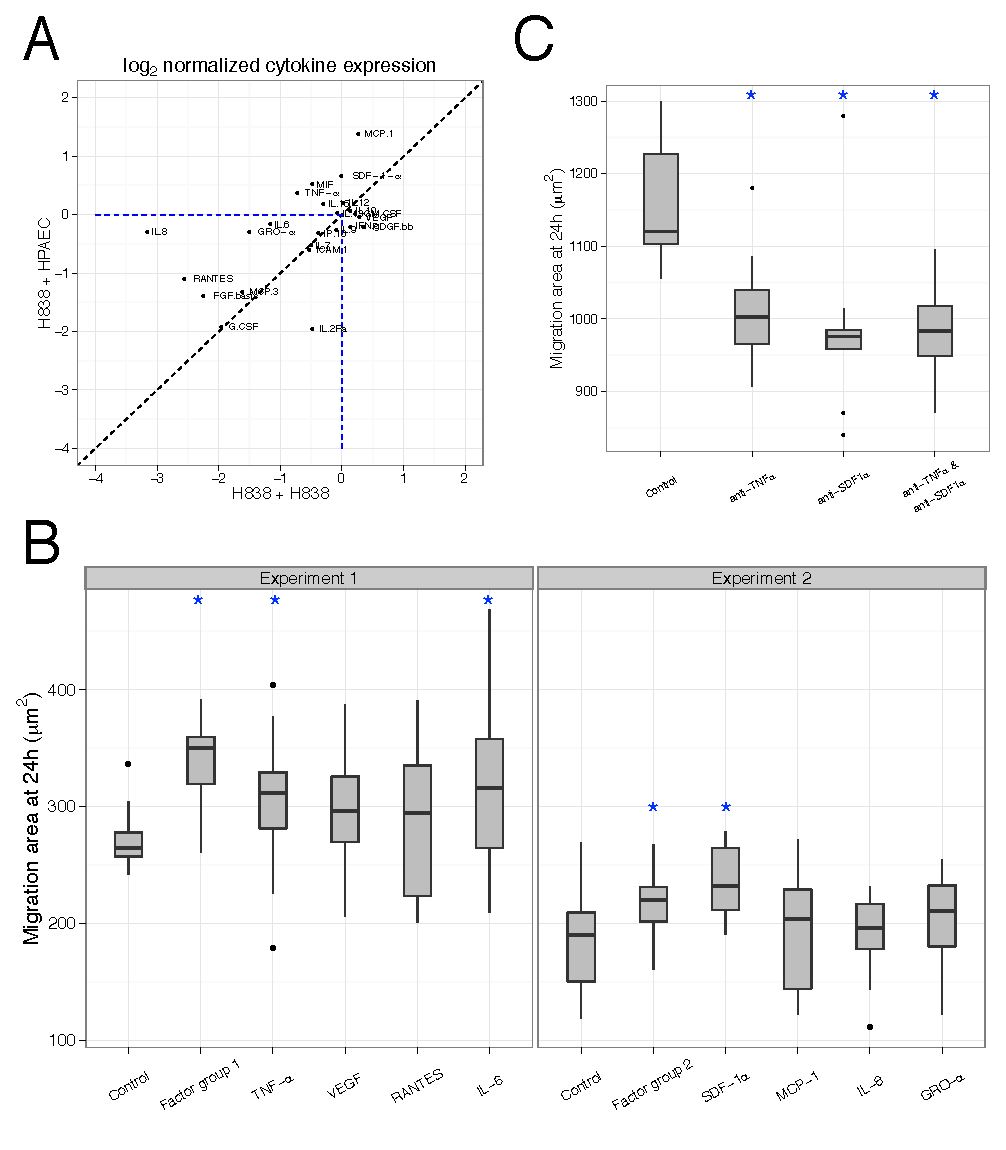
\includegraphics[width=\textwidth]{fig-cytokine.pdf}
\end{center}
\caption[Verification of key cytokines]{
{\bf Verification of key cytokines involved in the tumor cell migration.} 
(A) $\log_2$ transformed ratios of cytokine expression in heterogeneous respective
homogeneous coculture are shown. The black dashed line with a slope of 1 denotes 
the identity and the blue dashed lines denote the zero $\log_2$ fold change
or equal amount of cytokines between the scratched and unscratched conditioned 
media.
(B) Migration area of H838 cells at 24h after scratch in the H838 mono-culture 
treated with the 8
factors, the 2 factor groups and as in the control experiment.
(C) Migration area of H838 cells at 24h after scratch in the heterogeneous 
H838/HPAEC coculture 
treated with the neutralizing antibodies against TNF-$\alpha$, SDF-1$\alpha$
and both together. Asterisks in all plots denote that data are significantly 
different from the control according to a two-sided $t$-test ($p < 0.05$).
}
\label{fig:cytokine}
%\end{center}
\end{figure}

\subsubsection{Cytokine genes are expressed differently in H838 and HPAEC}

To elucidate the origin of the differential cytokine concentrations,
we investigated the gene expression profiles of
our previously identified cytokines of interest in H838 cells. 
%We compared the basal 
%expression levels of all genes with protein products
%annotated as cytokines in the KEGG cytokine-cytokine receptor interaction pathway. 
%However, none of the cytokine encoding genes 
%showed a differential basal regulation between the two coculture conditions. Over time, IL6 and CXCL14 are significantly
%down-regulated, and CSF1 is significantly up-regulated. 
Both \tnfa and \sdfonea do
not respond differentially during H838 migration (\ref{fig:cytokine_dynamic} A)
% maybe put this figure into the supplement
%Looking at the basal expression levels within each culture condition, only five out of 162 cytokines (IL18, IL10, PDGFC, BMP7 and TNFSF12) 
%had a significantly high expression level in both conditions
%(\ref{fig:cytokine_basal}), 
%and none of these could be directly related to the migration-enhancing 
%cell-cell communication.

%\begin{figure}[!ht]
\begin{center}
\captionsetup{labelformat=prepage}
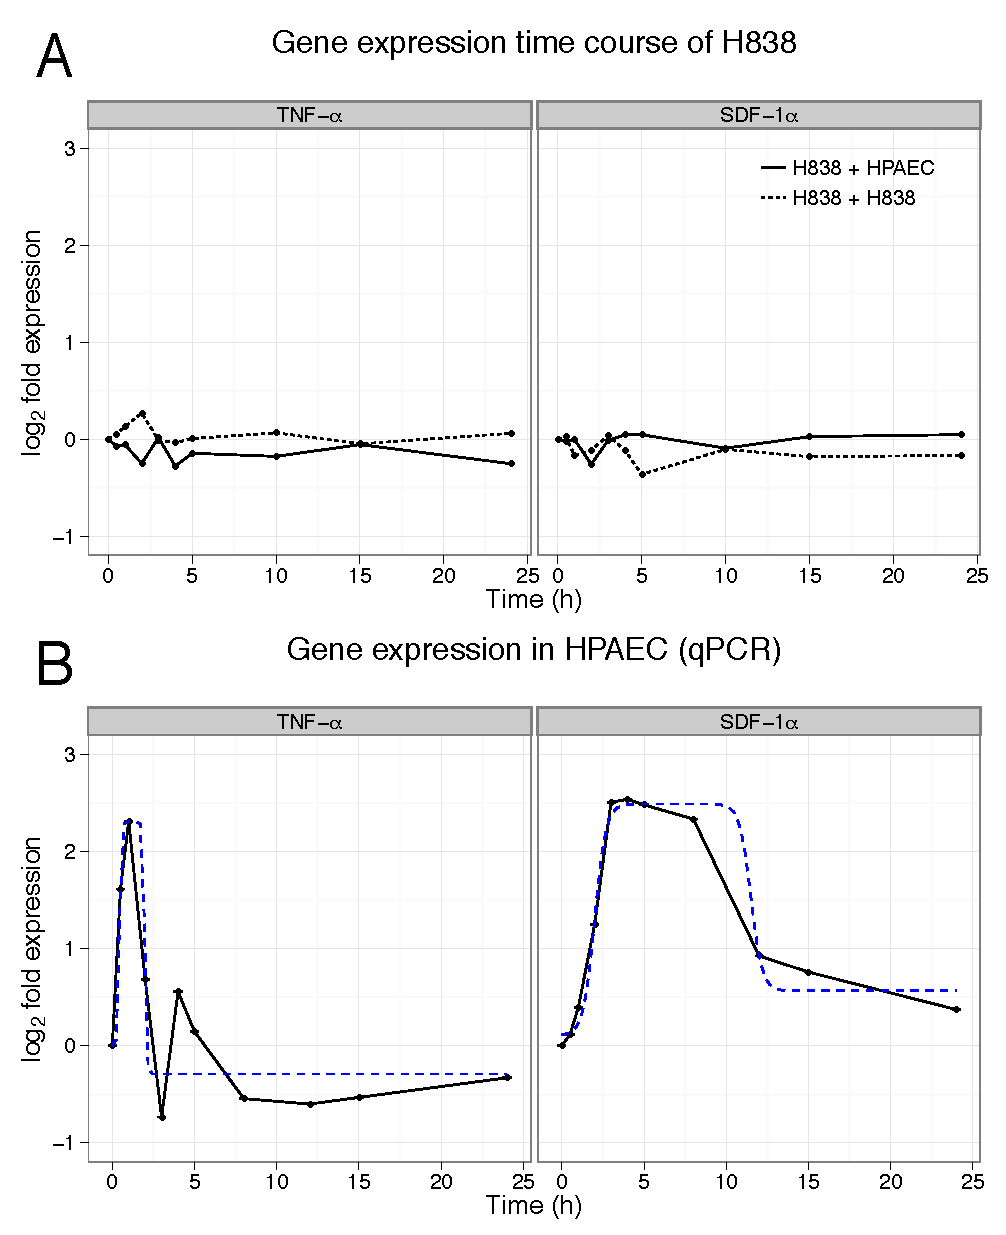
\includegraphics[width=\textwidth]{fig-cytokine_dynamic.pdf}
\newpage
%\end{center}
\captionof{figure}[Gene expression of \tnfa and \sdfonea]{
{\bf mRNA of TNF-$\alpha$ and SDF-1$\alpha$ is regulated in HPAEC instead of H838 
cells.}
(A) $\log_2$ fold expression of TNF-$\alpha$ and SDF-1$\alpha$ (CXCL12) in H838 
cells plotted
over time for the hetero- and homogeneous coculture respectively.
(B) $\log_2$ fold expression of TNF-$\alpha$ and SDF-1$\alpha$ in HPAEC cells 
from the qPCR
experiment in the heterogeneous coculture plotted
over time. Blue dashed lines denote the impulse model fit~\cite{Chechik2009}.
}
\label{fig:cytokine_dynamic}
%\end{figure}
\end{center}

%\begin{figure}[!ht]
%\begin{center}
%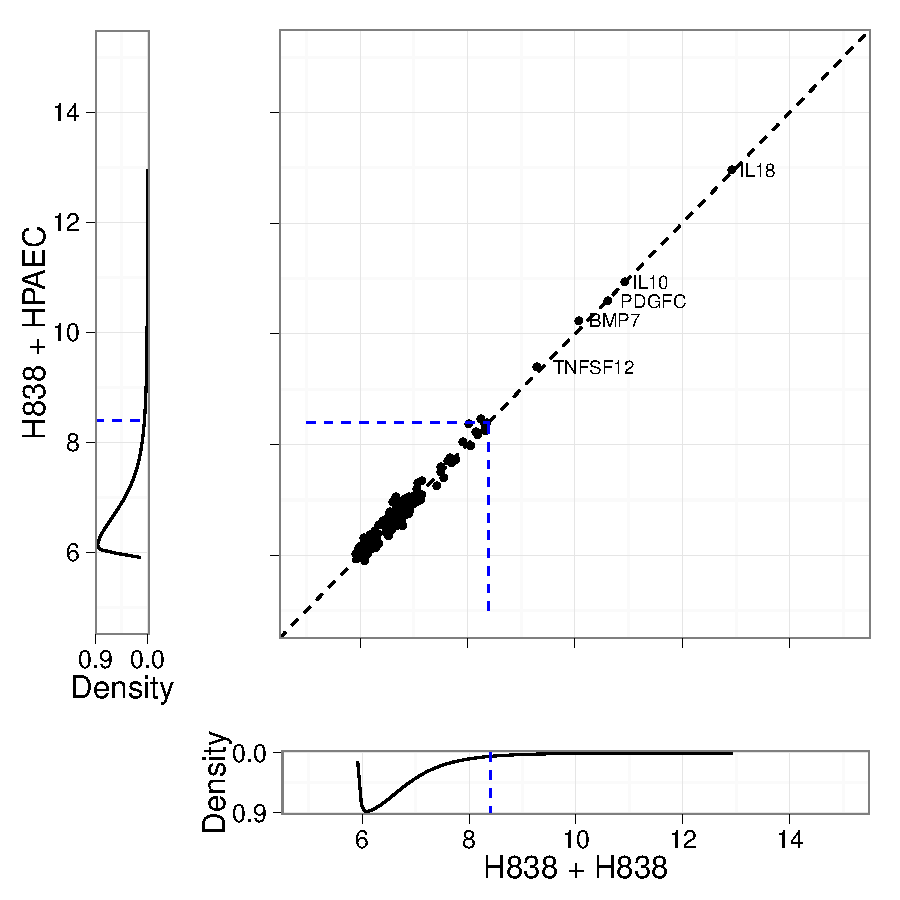
\includegraphics[width=\textwidth]{fig-basal_cytokine.pdf}
%\end{center}
%\caption[Basal cytokine gene expression]{
%{\bf Few cytokines highly expressed in H838 at 0h.}
%Comparison of $\log_2$ transformed basal mRNA intensities at 0h of all 
%cytokines annotated 
%in the KEGG \emph{cytokine-cytokine receptor interaction pathway} between
%the hetero- and homogeneous coculture. Blue dashed lines denote the significance
%level ($p=0.05$) after fitting the basal expression distribution with a skew-$t$ 
%distribution~\cite{Azzalini2003}. Only IL18, IL10, PDGFC,
%BMP7 and TNFSF12 are above this threshold in both conditions, 
%i.e. significantly up-regulated
%at 0h.
%}
%\label{fig:cytokine_basal}
%\end{figure}

We conclude that differential cytokine regulation in the supernatant 
must originate primarily from the HPAEC cells.  
An RT-qPCR experiment confirmed an early and transient response of  
TNF-$\alpha$ as well as a later and prolonged upregulation of 
SDF-1$\alpha$ (\ref{fig:cytokine_dynamic} B). 
Fitting the time course with an impulse model, which measures the peak 
duration as the 
temporal difference between the inflection points of two
sigmoidal curves, 
% add this in materials and methods
we obtain an activation duration of  8.3 hours and 1.6 hours for SDF-1$\alpha$
and TNF-$\alpha$, respectively.

\subsection{Discussion}

The key medical problem in lung cancer and its predominant type non-small 
cell lung carcinoma (NSCLC) is an early systemic metastatic spread of tumor cells 
independent of tumor size, which leads to high mortality rate. Tumor progression 
and metastasis is regulated by many different processes, inter alia by interactions 
via soluble factors between tumor cells and cells of tumor microenvironment, such as 
endothelial cells. In this study, we analyzed the interactions between NSCLC cells 
and endothelial cells and their influence on NSCLC cell migration. We identified 
two key cytokines, TNF-$\alpha$ and SDF-1$\alpha$, that are expressed by the 
endothelial cells and promote the migration of NSCLC cells.

In this study, we verified that TNF-$\alpha$ and SDF-1$\alpha$ are two
key cytokines that are expressed by the endothelial cells and promote the migration
of tumor cells. We proposed a two-step approach to link the transcriptome response
with the causal signal flow in the protein interaction network. First, gene set
enrichment analysis was applied to infer the sequence of transcription factor
activation that results in the gene expression. Second, we predicted several
putative receptors that are most closely linked to the downstream transcription
factors from the 
shortest path in the interactome. Among all candidate receptors,
TNF-$\alpha$ and SDF-1$\alpha$ receptors have a direct effect on the phenotype,
and the inhibition of the respective ligands leads to reduced migration 
activity. We further
hint at endothelial cells as possible sources for \tnfa and \sdfonea.

We discuss next about endothelial cell-tumor cell communication, what is known and what we found at transcription and protein level.
Then about the role of \tnfa and \sdfonea in tumors and especially lung tumors.

\begin{itemize}
\item \textbf{What do we know about \tnfa and \sdfonea with respect to cell migration?}

\tnfa was first identified as an anti-tumor cytokine that is involved in the killing
of certain kinds of tumors, however, it is appreciated recently that \tnfa can also 
act as a tumor-promoting factor and enhance tumor growth and metastasis%
~\citep{Wu2010}. It has also been shown in the ovarian cancer cells cocultured with
macrophages that \tnfa can induce the up-regulation of 
CXCR4 mRNA, which is the receptor of \sdfonea. This response to \tnfa involves both
AP-1 and NF-$\kappa$B related pathways~\citep{Kulbe2005}. Blocking the \tnfa receptor
in mouse Lewis lung carcinoma cell cultures decreases the gene expression of CXCR4~%
\citep{Sasi2011}.

It has been shown that the \sdfonea/CXCR4 pathway has pleiotropic activities and it 
promotes tumor growth and malignancy, enhances tumor angiogenesis, participates in tumor metastasis, and contributes to immunosuppressive networks within the tumor microenvironment~\citep{Kryczek2007}. 
Recently, it has also been shown that a special NSCLC cell line expresses a
high amount of CXCR4 and has cancer stem-like cell functions. The CXCR4-mediated
signaling is likely relayed by STAT3~\citep{Jung2013}.
Both stroma and cancer cells can produce \sdfonea, 
although in our system it is mainly expressed by the endothelial cells. In the presence of neutralizing \sdfonea antibodies, NSCLC tumor metastases were also significantly reduced~\citep{Phillips2003}.

The identification of \tnfa as a key stroma-originating factor that promotes 
tumor cell migration is of great interest, since its release is a general response to chemotherapy in different stromal cell types~\citep{Acharyya2012}. Together with
other cytokines, such as HGF, that contribute to the drug resistance of cancer
treatment~\citep{Straussman2012}, these soluble factors in the tumor microenvironment
might be the key to the cancer therapy and the potential target of intervention.


\item \textbf{What is new in our methods?}

The advantage of our two-step approach to identifying signal flow in the protein 
interaction
network and relevant transcription factors that lead to the transcriptome response
is at least two-fold: first, we apply gene set enrichment test to avoid the hard 
significance cutoff in the conventional hypergeometric test and at the same time
to detect weak but coordinated regulation of transcription factor targets. This is 
necessary since the tumor cell transcriptome does not show significantly
differential regulation between the homo- and heterogeneous coculture 
(\ref{fig:h838_transcriptome}), which 
hints at a lack of correlation between the mRNA expression level and the protein 
activity. This in turn underlines the rationale behind the time-scale separation
in our approach. Second, due to the decoupling between the mRNA and protein
activities, it is vital to consider signaling pathways not directly represented
in the transcriptome data, but rather embedded in the protein interaction network
instead. In order to infer the signal flow from the membrane receptors to 
transcription factors, we simply assume that the signal traverses the shortest
path connecting a certain pair of receptor and transcription factor.

\item \textbf{What new  biology do we find?}

Based on our time-resolved qPCR results, we conclude that \tnfa in the endothelial 
cells is 
transiently expressed and peaks earlier than \sdfonea, whereas the latter has
a longer activation time window. These results are in line with the hypothesis 
that \tnfa induces the CXCR4 expression in tumor cells, which can then respond
to \sdfonea. Nevertheless, CXCR4 in the lung cancer cell line H838 is neither
basal highly expressed (Benjamini-Hochberg corrected $p$-value = 0.7977245), nor differentially regulated over time (Benjamini-Hochberg
corrected $p$-value = 0.893767) in the 
heterogeneous coculture of tumor and endothelial cells, which indicates that
cytokine receptors important for the communication with endothelial cells might
only be regulated at the protein level.

According to the transcription factor target enrichment analysis, target genes
of AP-1 are more significantly upregulated within the first two hours. 
%whereas those
%of NF-$\kappa$B are only activated between 12 and 16 hours, although both AP-1 and
%NF-$\kappa$B are known to be involved in the \tnfa induced response~%
%\citep{Kulbe2005}. 
Taking into account
the early expression peak of \tnfa in the endothelial cells, it seems
in our particular coculture system of H838 and HPAEC cells, the initial 
transcriptome response in the tumor cells might be mediated through the AP-1
related pathway~\citep{Kulbe2005}. It has also been
shown that the CXCL12/CXCR4 activation of NSCLC cell lines 
increased intracellular calcium mobilization and MAP kinase 
activation with enhanced ERK1/2 phosphorylation~%
\citep{Belperio2004}, which is 
known to be upstream of the AP-1 transcription complex.
Therefore, all evidence points to the important role of the
AP-1 complex in the tumor cells to convey the information of  
the \sdfonea/CXCR4 activation from the microenvironment and to initiate cell
migration~\citep{Busch2008,Singh2012}.

Cell-cycle related transcription factors E2F has been linked with the chemokine
receptor CXCR4 in neurons. The transcriptional activity of E2F is either 
increased or decreased depending on the type of the CXCR4 ligand~\citep{Khan2003}.
The identification of E2F family proteins as activated transcription factors 
between 3 and 10 hours in the tumor cell also correlates with the expression of 
the CXCR4 ligand \sdfonea by endothelial cells within the same time frame.

%By analyzing the shortest paths between receptors and transcription factors, 
%we classified \tnfa and \sdfonea related 
%pathways into the homogeneous and
%heterogeneous response pattern respectively. Taking into account the different
%expression dynamics of both cytokines in the endothelial cells, this implies a
%complementary role \tnfa and \sdfonea play in the enhancement of lung cancer
%cell migration. It could be that the transient expression of \tnfa by the 
%endothelial cells initiates a first but unspecific response in the tumor cells,
%while the secondary prolonged stimulation from \sdfonea leads to a signal that 
%propagates preferentially 
%on a more specific set of paths to the downstream transcription factors, which
%ultimately determines \emph{point of no return} of the enhanced migration phenotype 
%in the tumor cells.

\begin{figure}[!ht]
\hskip 0.5in A \hskip 2.5in B
\begin{center}
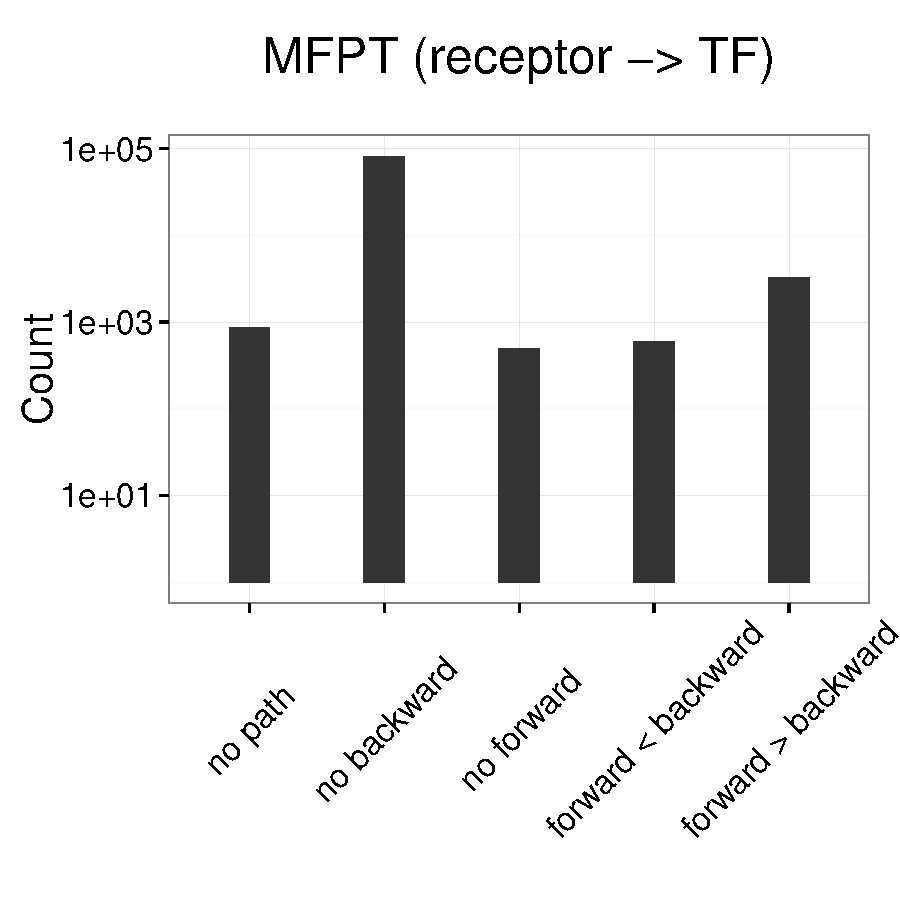
\includegraphics[width=0.45\textwidth]{mfpt-directed_bar.pdf}
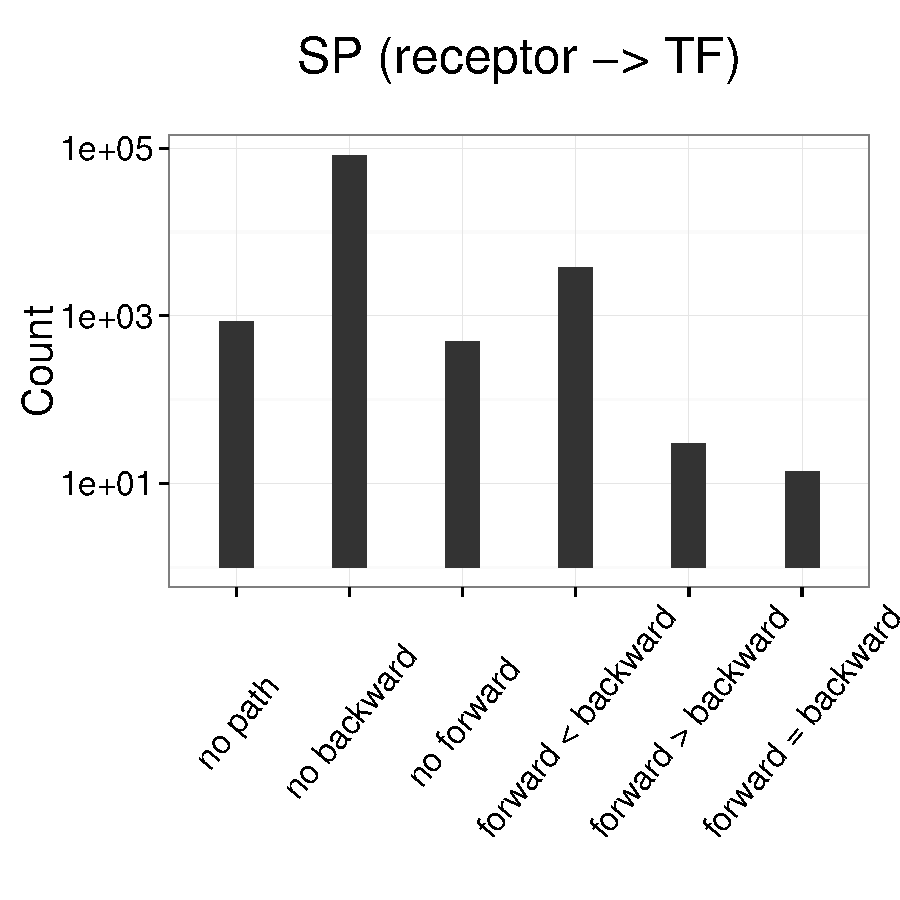
\includegraphics[width=0.45\textwidth]{sp-directed_bar.pdf}
\end{center}
\caption[Differential basal and dynamic gene expression]{
{\bf Differential basal and dynamic gene expression in homo- and heterogeneous 
cocultures.} 
(A) Histogram of the differential gene expression at 0h as determined by limma~%
\citep{Smyth2004}. 
Basal differential expression is 
represented as the negative log-transformed and multiple
testing corrected $p$-value of the limma test.
(B) Histogram of the differential gene expression over time as determined by the
full/reduced model fitting~\citep{Mar2009}.
Dynamical differential expression is 
represented as the negative log-transformed and multiple
testing corrected $p$-value of the full/reduced model
likelihood ratio test.
}
\label{fig:mfpt_sp_bar}
\end{figure}

\end{itemize}










%\cleardoublepage{}
%
%\lhead[\fancyplain{}{}]{\fancyplain{}{Acknowledgments}}
%
%\rhead[\fancyplain{}{Acknowledgments}]{\fancyplain{}{}}
%
%
%
%\include{Appendix}

\cleardoublepage{}

\lhead[\fancyplain{}{}]{\fancyplain{}{\rightmark}}

\rhead[\fancyplain{}{\leftmark}]{\fancyplain{}{}}

\bibliographystyle{natbib}
\bibliography{diss,network/network,flow/flow}

\cleardoublepage{}

\lhead[\fancyplain{}{}]{\fancyplain{}{Nomenclature}}
\rhead[\fancyplain{}{Nomenclature}]{\fancyplain{}{}}

\printnomenclature{}

\chapter*{Acknowledgements}
\addcontentsline{toc}{chapter}{Acknowledgements}

%First off, I am grateful that Prof.~Ad Aertsen offered me this opportunity to 
%perform this work in the BrainWorks group. He not only oversees the whole 
%project, but discusses with me about the progress on a regular basis as well. 
%
%Dr.~Ralph Meier initiated the whole project and guided me through all the 
%essential literature concerning various hippocampal models of epilepsy.
%He also built a bridge between me and other experienced researchers in
%this field and allowed me to freely explore something new.
%
%I want to thank Dr.~Thomas Fucke, without whom the completion of this
%work would not have been possible. His stimulating ideas and constant
%encouragement are very much appreciated. Besides, Thomas' easy-going
%character makes him an ideal person to share an office with.
%
%There are numerous people, both experimentalists and theoreticians, 
%whom I have had discussion with and who have read
%and commented on the working copies of this thesis. I am also 
%fond of all the ``balcony breaks''.
%
%I am thankful to Huili, who is a good company and makes my life
%more colorful; to my parents for their unconditional support.

\newpage
\chapter*{Erkl\"arung}
\addcontentsline{toc}{chapter}{Declaration}
\begin{enumerate}
\item Ich erkl\"are hiermit, dass ich die vorliegende Arbeit ohne unzul\"assige Hilfe Dritter und ohne Benutzung anderer als der angegebenen Hilfsmittel angefertigt habe. Die aus anderen Quellen direkt 
oder indirekt \"ubernommenen Daten und Konzepte sind unter Angabe der Quellen gekennzeichnet. Insbesondere habe ich hierf\"ur 
nicht die entgeltliche Hilfe von Vermittlungs- beziehungsweise 
Beratungsdiensten (Promotionsberater oder anderer Personen) 
in Anspruch genommen. Niemand hat von mir unmittelbar oder 
mittelbar geldwerte Leistungen f\"ur Arbeiten erhalten, die im Zusammenhang mit dem Inhalt der vorgelegten Dissertation stehen.
\item Die Arbeit wurde bisher weder im In- noch im Ausland in gleicher 
oder \"ahnlicher Form einer anderen Pr\"ufungsbeh\"orde vorgelegt.
\item Die Bestimmungen der Promotionsordnung der Fakult\"at f\"ur Biologie der Universit\"at Freiburg sind mir bekannt, insbesondere 
wei\ss ich, dass ich vor Vollzug der Promotion zur F\"uhrung des 
Doktortitels nicht berechtigt bin.
\end{enumerate}
\vskip 3cm
Freiburg, den \ddmmyyyydate\today \hspace{6cm} Jie Bao

\end{document}
